\documentclass[a4paper, openany]{memoir}

\usepackage[utf8]{inputenc}
\usepackage[T1]{fontenc} 
\usepackage[english]{babel}

\usepackage{fancyhdr}
\usepackage{float}

\usepackage{amsmath}
\usepackage{amsthm}
\usepackage{amssymb}
\usepackage{enumitem}
\usepackage{multicol}
\usepackage[bookmarksopen=true,bookmarksopenlevel=2]{hyperref}
\usepackage{tikz}
\usepackage{tikz-qtree}
\usepackage{indentfirst}

\usepackage{listings}
\usepackage{xcolor}

\pagestyle{fancy}
\fancyhf{}
\fancyhead[LE]{\leftmark}
\fancyhead[RO]{\rightmark}
\fancyhead[RE, LO]{ADS}
\fancyfoot[LE, RO]{\thepage}
\fancyfoot[RE, LO]{Pete Gautam}

\definecolor{codegreen}{rgb}{0,0.6,0}
\definecolor{codegray}{rgb}{0.5,0.5,0.5}
\definecolor{codepurple}{rgb}{0.58,0,0.82}
\definecolor{backcolour}{rgb}{0.95,0.95,0.92}

\lstdefinestyle{thestyle}{
    backgroundcolor=\color{backcolour},
    basicstyle=\ttfamily\footnotesize,
    keywordstyle=\color{red!80}\bfseries,
    ndkeywordstyle=\color{blue!80}\bfseries,
    identifierstyle=\color{black},
    commentstyle=\color{codegreen},
    stringstyle=\color{codepurple},
    breakatwhitespace=false,
    breaklines=true,
    captionpos=b,
    keepspaces=true,
    numberstyle=\tiny\color{codegray},
    numbers=left,
    numbersep=2pt,
    showspaces=false,
    showstringspaces=false,
    showtabs=false,
    tabsize=2
}
\lstset{style=thestyle}

\lstdefinelanguage{pseudocode}{ 
    keywords={new, return, this, null, if, in, while, else, for, get, set, class, and, or, not, range, Function, throw},
    ndkeywords={int, char, bool, Array, String, Node, Queue, Set, void, true, false, LinkedArray, CLinkedArray, Stack, Dequeue, List, BNode, BST, Tree, Map, MapEntry},
    sensitive=true,
    comment=[l]{//},
    morecomment=[s]{/*}{*/},
    morestring=[b]',
    morestring=[b]"
}


\renewcommand{\headrulewidth}{1.5pt}

\tikzset{every tree node/.style={minimum width=2em,draw},
 blank/.style={draw=none},
 edge from parent/.style=
 {draw,edge from parent path={(\tikzparentnode) -- (\tikzchildnode)}},
 level distance=1.5cm,
 black/.style={draw=black},
 }
\usetikzlibrary{backgrounds}
\usetikzlibrary{shapes}

\chapterstyle{thatcher}
\setcounter{chapter}{1}

\begin{document}
\chapter{Data Structures}
\section{Linked List}
A data structure stores data that helps us access them for a particular need. We use a wide variety of data structures since a single data structure isn't useful for all the requirements, e.g. array, set, queue, tree, stack. 

\noindent Just sticking with arrays is a bad idea. For example, we cannot dynamically add or delete to an array- we would need to resize the array and copy all the elements. Also, a lot of memory might be allocated, but not much of that might be used in an array. For that reason, we seek other dynamic data structures, like a linked list. 

\noindent A linked list is the simplest type of a dynamic data structure. A linked list is made up of nodes with a pointer to another node(s).

\subsection{Singly Linked List}
A singly linked list, or just a linked list, is a sequence of nodes arranged in linear order. Every node has a pointer to the next node. For example, the following is a linked list:
\begin{center}
    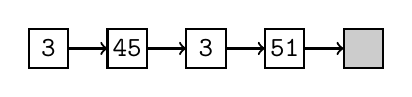
\begin{tikzpicture}
        \foreach \x[count=\i] in {3, 45, 3, 51} {
            \draw[thick] (\i-1, 0) -- (\i-1, .5) -- (\i-.5, .5) -- (\i-.5, 0) -- cycle;
            \draw[thick, ->] (\i-.5, .25) -- (\i, .25);
            \node at (\i-.75, .25) {\texttt{\x}};
        }
        \draw[thick, fill=gray!40] (4, 0) -- (4, .5) -- (4.5, .5) -- (4.5, 0) -- cycle;
    \end{tikzpicture}
\end{center}
Every node is represented by a square. The arrow represents whether the attribute \texttt{next} of the node points. The tail in the array points to \texttt{null}. We refer to the first element in the linked list by \texttt{head}. In this case, the node corresponding to \texttt{head} has value \texttt{3}.

\subsubsection{Insert}
\noindent Now, we consider addition of a node into a linked list at the head. The following is the pseudocode:
\begin{lstlisting}[language=pseudocode]
void insert<E>(LinkedArray<E> array, Node<E> node):
    node.next = array.head
    array.head = node
\end{lstlisting}
Here, we set the \texttt{next} attribute of the \texttt{node} to the \texttt{head} of the array. Then, we set the \texttt{head} of the array to be the new node. This function has complexity $O(1)$.

\noindent Assume we start with an empty linked list and add two nodes with values \texttt{2} and \texttt{3}.
\begin{center}
    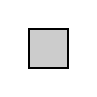
\begin{tikzpicture}
        \draw[thick, fill=gray!40] (0, 0) -- (0, .5) -- (.5, .5) -- (.5, 0) -- cycle;
    \end{tikzpicture}
\end{center}
We start with an empty linked list.
\begin{center}
    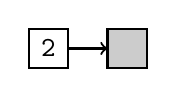
\begin{tikzpicture}
        \draw[thick] (0, 0) -- (0, .5) -- (.5, .5) -- (.5, 0) -- cycle;
        \draw[thick, ->] (.5, .25) -- (1, .25);
        \node at (.25, .25) {\texttt{2}};
        
        \draw[thick, fill=gray!40] (1, 0) -- (1, .5) -- (1.5, .5) -- (1.5, 0) -- cycle;
        \end{tikzpicture}
\end{center}
To the empty array, we first add a node with value \texttt{2}. That is, the \texttt{next} attribute of the \texttt{node} becomes the previous \texttt{head} \texttt{null}. This also implies that \texttt{2} is where the array ends. Then, the \texttt{head} of the array becomes the \texttt{next}.
\begin{center}
    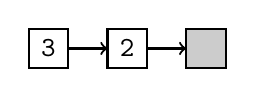
\begin{tikzpicture}
        \draw[thick] (0, 0) -- (0, .5) -- (.5, .5) -- (.5, 0) -- cycle;
        \draw[thick, ->] (.5, .25) -- (1, .25);
        \node at (.25, .25) {\texttt{3}};
        
        \draw[thick] (1, 0) -- (1, .5) -- (1.5, .5) -- (1.5, 0) -- cycle;
        \draw[thick, ->] (1.5, .25) -- (2, .25);
        \node at (1.25, .25) {\texttt{2}};
        
        \draw[thick, fill=gray!40] (2, 0) -- (2, .5) -- (2.5, .5) -- (2.5, 0) -- cycle;
    \end{tikzpicture}
\end{center}
Next, we add the element \texttt{3} at the start. \texttt{2} gets pushed to the next element, and the array now has 2 elements.

\subsubsection{Delete}
\noindent We now consider deletion of a node from the head. The following is the pseudocode:
\begin{lstlisting}[language=pseudocode]
void delete<E>(LinkedArray<E> array):
    if (array.head != null):
        array.head = array.head.next
\end{lstlisting}
We move the \texttt{head} of the array to the \texttt{next} element. That way, the \texttt{head} element becomes removed from the array. This function has complexity $O(1)$.

\noindent Assume we now call the \texttt{delete} function on the array \texttt{[3, 2]} twice.
\begin{center}
    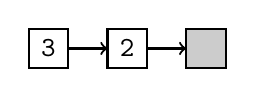
\begin{tikzpicture}
        \draw[thick] (0, 0) -- (0, .5) -- (.5, .5) -- (.5, 0) -- cycle;
        \draw[thick, ->] (.5, .25) -- (1, .25);
        \node at (.25, .25) {\texttt{3}};
        
        \draw[thick] (1, 0) -- (1, .5) -- (1.5, .5) -- (1.5, 0) -- cycle;
        \draw[thick, ->] (1.5, .25) -- (2, .25);
        \node at (1.25, .25) {\texttt{2}};
        
        \draw[thick, fill=gray!40] (2, 0) -- (2, .5) -- (2.5, .5) -- (2.5, 0) -- cycle;
    \end{tikzpicture}
\end{center}
We start with the array with all 3 elements.
\begin{center}
    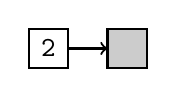
\begin{tikzpicture}
        \draw[thick] (0, 0) -- (0, .5) -- (.5, .5) -- (.5, 0) -- cycle;
        \draw[thick, ->] (.5, .25) -- (1, .25);
        \node at (.25, .25) {\texttt{2}};
        
        \draw[thick, fill=gray!40] (1, 0) -- (1, .5) -- (1.5, .5) -- (1.5, 0) -- cycle;
        \end{tikzpicture}
\end{center}
When we first call delete, we set the \texttt{head} of the array to be the \texttt{next} element \texttt{2}.
\begin{center}
    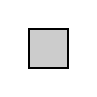
\begin{tikzpicture}
        \draw[thick, fill=gray!40] (0, 0) -- (0, .5) -- (.5, .5) -- (.5, 0) -- cycle;
    \end{tikzpicture}
\end{center}
Calling delete again makes the array empty. Any further call to delete doesn't make a change to the array.

\subsubsection{Search}
We now consider searching a value within the array. The function returns the first node containing the required value, if it is found. If not, it returns \texttt{null}. This is a simple linear search that iterates through the array, finding a node with that value. The pseudocode is:
\begin{lstlisting}[language=pseudocode]
Node<E> search<E>(LinkedArray<E> array, E value):
    Node<E> node = array.head
    while (node != null && node.value != k):
        node = node.next
    return node
\end{lstlisting}
We show how the function works by finding the node with value \texttt{3} from the linked list \texttt{[1, 3, 3, 5]}.
\begin{center}
    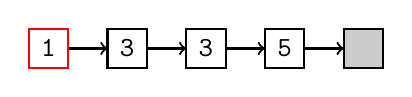
\begin{tikzpicture}
        \foreach \x[count=\i] in {1, 3, 3, 5} {
            \draw[thick, ->] (\i-.5, .25) -- (\i, .25);
            \node at (\i-.75, .25) {\texttt{\x}};
        }
        \draw[thick, red] (0, 0) -- (0, .5) -- (.5, .5) -- (.5, 0) -- cycle;
        \draw[thick] (1, 0) -- (1, .5) -- (1.5, .5) -- (1.5, 0) -- cycle;
        \draw[thick] (2, 0) -- (2, .5) -- (2.5, .5) -- (2.5, 0) -- cycle;
        \draw[thick] (3, 0) -- (3, .5) -- (3.5, .5) -- (3.5, 0) -- cycle;
        \draw[thick, fill=gray!40] (4, 0) -- (4, .5) -- (4.5, .5) -- (4.5, 0) -- cycle;
    \end{tikzpicture}
\end{center}
Originally, the value of \texttt{node} is the first node. Since it isn't a \texttt{null} node and its \texttt{value} isn't 1, we continue the while loop.
\begin{center}
    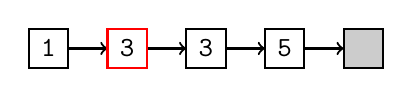
\begin{tikzpicture}
        \foreach \x[count=\i] in {1, 3, 3, 5} {
            \draw[thick, ->] (\i-.5, .25) -- (\i, .25);
            \node at (\i-.75, .25) {\texttt{\x}};
        }
        \draw[thick] (0, 0) -- (0, .5) -- (.5, .5) -- (.5, 0) -- cycle;
        \draw[thick, red] (1, 0) -- (1, .5) -- (1.5, .5) -- (1.5, 0) -- cycle;
        \draw[thick] (2, 0) -- (2, .5) -- (2.5, .5) -- (2.5, 0) -- cycle;
        \draw[thick] (3, 0) -- (3, .5) -- (3.5, .5) -- (3.5, 0) -- cycle;
        \draw[thick, fill=gray!40] (4, 0) -- (4, .5) -- (4.5, .5) -- (4.5, 0) -- cycle;
    \end{tikzpicture}
\end{center}
Now, since \texttt{3} is the value of this node, we return the node.

\noindent If we wanted to find \texttt{7} in the array, we would have ended up returning the final, \texttt{null} node.

\noindent The structure of a linked list allows for us to make it a recursive function. The psuedocode in that case is:
\begin{lstlisting}[language=pseudocode]
void search<E>(Node<E> node, E value):
    if (node == null):
        return node
    else if (node.value == k):
        return node
    return search(node.next, value)
\end{lstlisting}
We start the recursive call first with \texttt{array.head}.
\subsubsection{Search}
A sorting algorithm for a linked list cannot rely on accessing any index in constant time. So, we use merge sort to sort the linked list. This is a divide and conquer algorithm, involving splitting the array into sorted sublists and then merging the array. We first consider merging two sorted linked lists:
\begin{lstlisting}[language=pseudocode]
Node<int> merge(Node<int> node1, Node<int> node2):
    if (node1 == null):
        return node2
    else if (node2 == null):
        return node1
    Node<E> merged = null
    if (node1.value <= node2.value):
        merged = node1
        merged.next = merge(node1.next, node2)
    else:
        merged = node2
        merged.next = merge(node1, node2.next)
    return merged
\end{lstlisting}
Here, the two nodes are the heads of the two linked lists. The returned node is the head of the merged linked list. It recursively establishes the next element of the node by considering the highest element of the largest elements.

\noindent We now consider how the function merges the two arrays \texttt{[1, 3]} and \texttt{[2, 5]}.
\begin{center}
    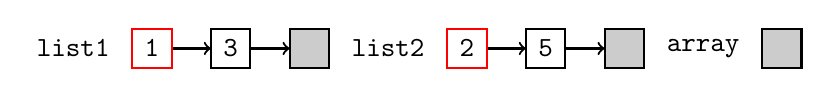
\begin{tikzpicture}
        \node at (-0.75, .25) {\texttt{list1}};
        \foreach \x[count=\i] in {1, 3} {
            \draw[thick, ->] (\i-.5, .25) -- (\i, .25);
            \node at (\i-.75, .25) {\texttt{\x}};
        }
        \draw[thick, red] (0, 0) -- (0, .5) -- (.5, .5) -- (.5, 0) -- cycle;
        \draw[thick] (1, 0) -- (1, .5) -- (1.5, .5) -- (1.5, 0) -- cycle;
        \draw[thick, fill=gray!40] (2, 0) -- (2, .5) -- (2.5, .5) -- (2.5, 0) -- cycle;
        
        \node at (3.25, .25) {\texttt{list2}};
        \foreach \x[count=\i] in {2, 5} {
            \draw[thick, ->] (4+\i-.5, .25) -- (4+\i, .25);
            \node at (4+\i-.75, .25) {\texttt{\x}};
        }
        \draw[thick, red] (4, 0) -- (4, .5) -- (4.5, .5) -- (4.5, 0) -- cycle;
        \draw[thick] (5, 0) -- (5, .5) -- (5.5, .5) -- (5.5, 0) -- cycle;
        \draw[thick, fill=gray!40] (6, 0) -- (6, .5) -- (6.5, .5) -- (6.5, 0) -- cycle;
        
        \node at (7.25, .25) {\texttt{array}};
        \draw[thick, fill=gray!40] (8, 0)  -- (8, .5) -- (8.5, .5) -- (8.5, 0) -- cycle;
    \end{tikzpicture}
\end{center}
We start with \texttt{list1} and \texttt{list2} with all the elements, and the merged \texttt{array} empty.
\begin{center}
    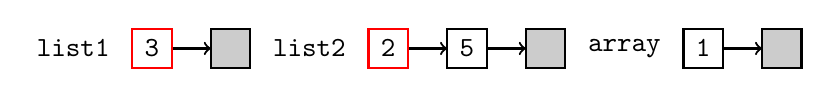
\begin{tikzpicture}
        \node at (-0.75, .25) {\texttt{list1}};
        \foreach \x[count=\i] in {3} {
            \draw[thick, ->] (\i-.5, .25) -- (\i, .25);
            \node at (\i-.75, .25) {\texttt{\x}};
        }
        \draw[thick, red] (0, 0) -- (0, .5) -- (.5, .5) -- (.5, 0) -- cycle;
        \draw[thick, fill=gray!40] (1, 0) -- (1, .5) -- (1.5, .5) -- (1.5, 0) -- cycle;
        
        \node at (2.25, .25) {\texttt{list2}};
        \foreach \x[count=\i] in {2, 5} {
            \draw[thick, ->] (3+\i-.5, .25) -- (3+\i, .25);
            \node at (3+\i-.75, .25) {\texttt{\x}};
        }
        \draw[thick, red] (3, 0) -- (3, .5) -- (3.5, .5) -- (3.5, 0) -- cycle;
        \draw[thick] (4, 0) -- (4, .5) -- (4.5, .5) -- (4.5, 0) -- cycle;
        \draw[thick, fill=gray!40] (5, 0) -- (5, .5) -- (5.5, .5) -- (5.5, 0) -- cycle;
        
        \node at (6.25, .25) {\texttt{array}};
        \foreach \x[count=\i] in {1} {
            \draw[thick, ->] (7+\i-.5, .25) -- (7+\i, .25);
            \node at (7+\i-.75, .25) {\texttt{\x}};
        }
        \draw[thick] (7, 0)  -- (7, .5) -- (7.5, .5) -- (7.5, 0) -- cycle;
        \draw[thick, fill=gray!40] (8, 0)  -- (8, .5) -- (8.5, .5) -- (8.5, 0) -- cycle;
    \end{tikzpicture}
\end{center}
Out of the \texttt{head} nodes \texttt{1} and \texttt{2}, \texttt{1} was smaller. So, we first add \texttt{1} to the \texttt{array}.
\begin{center}
    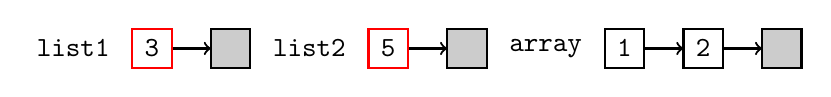
\begin{tikzpicture}
        \node at (-0.75, .25) {\texttt{list1}};
        \foreach \x[count=\i] in {3} {
            \draw[thick, ->] (\i-.5, .25) -- (\i, .25);
            \node at (\i-.75, .25) {\texttt{\x}};
        }
        \draw[thick, red] (0, 0) -- (0, .5) -- (.5, .5) -- (.5, 0) -- cycle;
        \draw[thick, fill=gray!40] (1, 0) -- (1, .5) -- (1.5, .5) -- (1.5, 0) -- cycle;
        
        \node at (2.25, .25) {\texttt{list2}};
        \foreach \x[count=\i] in {5} {
            \draw[thick, ->] (3+\i-.5, .25) -- (3+\i, .25);
            \node at (3+\i-.75, .25) {\texttt{\x}};
        }
        \draw[thick, red] (3, 0) -- (3, .5) -- (3.5, .5) -- (3.5, 0) -- cycle;
        \draw[thick, fill=gray!40] (4, 0) -- (4, .5) -- (4.5, .5) -- (4.5, 0) -- cycle;
        
        \node at (5.25, .25) {\texttt{array}};
        \foreach \x[count=\i] in {1, 2} {
            \draw[thick, ->] (6+\i-.5, .25) -- (6+\i, .25);
            \node at (6+\i-.75, .25) {\texttt{\x}};
        }
        \draw[thick] (6, 0)  -- (6, .5) -- (6.5, .5) -- (6.5, 0) -- cycle;
        \draw[thick] (7, 0)  -- (7, .5) -- (7.5, .5) -- (7.5, 0) -- cycle;
        \draw[thick, fill=gray!40] (8, 0)  -- (8, .5) -- (8.5, .5) -- (8.5, 0) -- cycle;
    \end{tikzpicture}
\end{center}
Since \texttt{2} is smaller than \texttt{3}, we add \texttt{2} into the \texttt{array}.
\begin{center}
    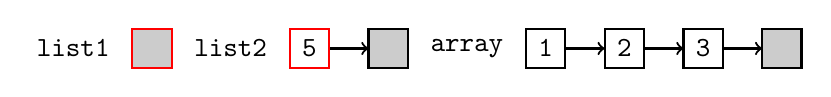
\begin{tikzpicture}
        \node at (-0.75, .25) {\texttt{list1}};
        \draw[thick, red, fill=gray!40] (0, 0) -- (0, .5) -- (.5, .5) -- (.5, 0) -- cycle;
        
        \node at (1.25, .25) {\texttt{list2}};
        \foreach \x[count=\i] in {5} {
            \draw[thick, ->] (2+\i-.5, .25) -- (2+\i, .25);
            \node at (2+\i-.75, .25) {\texttt{\x}};
        }
        \draw[thick, red] (2, 0) -- (2, .5) -- (2.5, .5) -- (2.5, 0) -- cycle;
        \draw[thick, fill=gray!40] (3, 0) -- (3, .5) -- (3.5, .5) -- (3.5, 0) -- cycle;
        
        \node at (4.25, .25) {\texttt{array}};
        \foreach \x[count=\i] in {1, 2, 3} {
            \draw[thick, ->] (5+\i-.5, .25) -- (5+\i, .25);
            \node at (5+\i-.75, .25) {\texttt{\x}};
        }
        \draw[thick] (5, 0)  -- (5, .5) -- (5.5, .5) -- (5.5, 0) -- cycle;
        \draw[thick] (6, 0)  -- (6, .5) -- (6.5, .5) -- (6.5, 0) -- cycle;
        \draw[thick] (7, 0)  -- (7, .5) -- (7.5, .5) -- (7.5, 0) -- cycle;
        \draw[thick, fill=gray!40] (8, 0)  -- (8, .5) -- (8.5, .5) -- (8.5, 0) -- cycle;
    \end{tikzpicture}
\end{center}
Now, \texttt{3} is smaller than \texttt{5}, so we add that node.
\begin{center}
    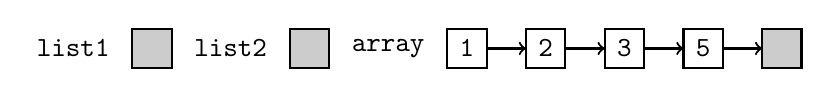
\begin{tikzpicture}
        \node at (-0.75, .25) {\texttt{list1}};
        \draw[thick, fill=gray!40] (0, 0) -- (0, .5) -- (.5, .5) -- (.5, 0) -- cycle;
        
        \node at (1.25, .25) {\texttt{list2}};
        \draw[thick, fill=gray!40] (2, 0) -- (2, .5) -- (2.5, .5) -- (2.5, 0) -- cycle;
        
        \node at (3.25, .25) {\texttt{array}};
        \foreach \x[count=\i] in {1, 2, 3, 5} {
            \draw[thick, ->] (4+\i-.5, .25) -- (4+\i, .25);
            \node at (4+\i-.75, .25) {\texttt{\x}};
        }
        \draw[thick] (4, 0)  -- (4, .5) -- (4.5, .5) -- (4.5, 0) -- cycle;
        \draw[thick] (5, 0)  -- (5, .5) -- (5.5, .5) -- (5.5, 0) -- cycle;
        \draw[thick] (6, 0)  -- (6, .5) -- (6.5, .5) -- (6.5, 0) -- cycle;
        \draw[thick] (7, 0)  -- (7, .5) -- (7.5, .5) -- (7.5, 0) -- cycle;
        \draw[thick, fill=gray!40] (8, 0)  -- (8, .5) -- (8.5, .5) -- (8.5, 0) -- cycle;
    \end{tikzpicture}
\end{center}
Since \texttt{list1} is empty, we add all the elements from \texttt{list2} into the \texttt{array}. The \texttt{array} is now sorted.

\noindent We now consider how we split the linked list into halves. We do this using two cursors- one cursor travels one node per iteration, while the second travels two nodes. So, at the end of the loop, the slow cursor is just before the midpoint.
\begin{lstlisting}[language=pseudocode]
[Node<int>, Node<int>] split(Node<int> node):
    if (node == null || a.next == null):
        return [node, null]
    Node<int> slow = node
    Node<int> fast = node.next
    while (fast != null && fast.next != null):
        slow = slow.next
        fast = fast.next.next
    Node<int> mid = slow.next
    slow.next = null
    return [node, mid]
\end{lstlisting}
We consider how the function splits the array \texttt{[1, 3, 3, 5]}.
\begin{center}
    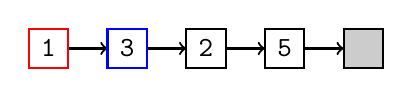
\begin{tikzpicture}
        \foreach \x[count=\i] in {1, 3, 2, 5} {
            \draw[thick, ->] (\i-.5, .25) -- (\i, .25);
            \node at (\i-.75, .25) {\texttt{\x}};
        }
        \draw[thick, red] (0, 0) -- (0, .5) -- (.5, .5) -- (.5, 0) -- cycle;
        \draw[thick, blue] (1, 0) -- (1, .5) -- (1.5, .5) -- (1.5, 0) -- cycle;
        \draw[thick] (2, 0) -- (2, .5) -- (2.5, .5) -- (2.5, 0) -- cycle;
        \draw[thick] (3, 0) -- (3, .5) -- (3.5, .5) -- (3.5, 0) -- cycle;
        \draw[thick, fill=gray!40] (4, 0) -- (4, .5) -- (4.5, .5) -- (4.5, 0) -- cycle;
    \end{tikzpicture}
\end{center}
This array has at least 2 elements, so we need to search the middle element. At the start, we have the two pointers- \texttt{slow} (red box) and \texttt{fast} (blue box). Since the blue node isn't the tail of the array, we move both the nodes.
\begin{center}
    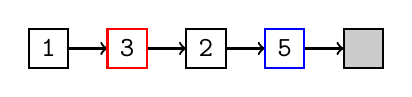
\begin{tikzpicture}
        \foreach \x[count=\i] in {1, 3, 2, 5} {
            \draw[thick, ->] (\i-.5, .25) -- (\i, .25);
            \node at (\i-.75, .25) {\texttt{\x}};
        }
        \draw[thick] (0, 0) -- (0, .5) -- (.5, .5) -- (.5, 0) -- cycle;
        \draw[thick, red] (1, 0) -- (1, .5) -- (1.5, .5) -- (1.5, 0) -- cycle;
        \draw[thick] (2, 0) -- (2, .5) -- (2.5, .5) -- (2.5, 0) -- cycle;
        \draw[thick, blue] (3, 0) -- (3, .5) -- (3.5, .5) -- (3.5, 0) -- cycle;
        \draw[thick, fill=gray!40] (4, 0) -- (4, .5) -- (4.5, .5) -- (4.5, 0) -- cycle;
    \end{tikzpicture}
\end{center}
Now, however, the blue node is the final node. So, we break the array at the location of the red node, and get the two arrays.
\begin{center}
    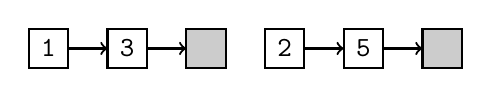
\begin{tikzpicture}
        \foreach \x[count=\i] in {1, 3} {
            \draw[thick, ->] (\i-.5, .25) -- (\i, .25);
            \node at (\i-.75, .25) {\texttt{\x}};
        }
        \draw[thick] (0, 0) -- (0, .5) -- (.5, .5) -- (.5, 0) -- cycle;
        \draw[thick] (1, 0) -- (1, .5) -- (1.5, .5) -- (1.5, 0) -- cycle;
        \draw[thick, fill=gray!40] (2, 0) -- (2, .5) -- (2.5, .5) -- (2.5, 0) -- cycle;
        
        \foreach \x[count=\i] in {2, 5} {
            \draw[thick, ->] (3+\i-.5, .25) -- (3+\i, .25);
            \node at (3+\i-.75, .25) {\texttt{\x}};
        }
        \draw[thick] (3, 0) -- (3, .5) -- (3.5, .5) -- (3.5, 0) -- cycle;
        \draw[thick] (4, 0) -- (4, .5) -- (4.5, .5) -- (4.5, 0) -- cycle;
        \draw[thick, fill=gray!40] (5, 0) -- (5, .5) -- (5.5, .5) -- (5.5, 0) -- cycle;
    \end{tikzpicture}
\end{center}
We return the \texttt{head} node of the two arrays.

\noindent Finally, we consider how the merge sort makes use of these functions:
\begin{lstlisting}[language=pseudocode]
Node<int> mergeSort(Node<int> node):
    if (node == null || node.next == null):
        return node
    [left, right] = split(node)
    Node<int> sortedl = mergeSort(left)
    Node<int> sortedr = mergeSort(right)
    return merge(sortedl, sortedr)
\end{lstlisting}
The function is called with the \texttt{head} of the linked list, and returns the head of the sorted linked list's \texttt{head}.

\subsubsection{Tail insertion}
If we wanted to add an element to the tail of the array, we need to traverse through the entire array. Therefore, it has complexity $O(n)$. The psuedocode for the insertion is:
\begin{lstlisting}[language=pseudocode]
void tailInsert<E>(LinkedArray<E> array, Node<E> node):
    if (array.head == null):
        insert(array, node)
    Node<E> prev = array.head
    while (prev.next != null):
        prev = prev.next
    prev.next = node
    node.next = null
\end{lstlisting}
Since this could be a common call on the linked list, it might not be the most efficient algorithm. We could add a pointer to the tail so the algorithm is linear. In that case, we need to update the functions \texttt{insert} and \texttt{delete}. Then, the \texttt{tailInsert} function becomes:
\begin{lstlisting}[language=pseudocode]
void tailInsert<E>(LinkedArray<E> array, Node<E> node):
    node.next = null
    if (array.tail == null):
        array.head = node
    else:
        array.tail.next = node
    array.tail = node
\end{lstlisting}
We consider how this function works by adding a node containing \texttt{6} to the tail of the linked list \texttt{[1, 3, 2, 5]}. Originally, we have the array
\begin{center}
    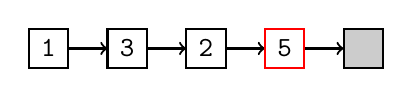
\begin{tikzpicture}
        \foreach \x[count=\i] in {1, 3, 2, 5} {
            \draw[thick, ->] (\i-.5, .25) -- (\i, .25);
            \node at (\i-.75, .25) {\texttt{\x}};
        }
        \draw[thick] (0, 0) -- (0, .5) -- (.5, .5) -- (.5, 0) -- cycle;
        \draw[thick] (1, 0) -- (1, .5) -- (1.5, .5) -- (1.5, 0) -- cycle;
        \draw[thick] (2, 0) -- (2, .5) -- (2.5, .5) -- (2.5, 0) -- cycle;
        \draw[thick, red] (3, 0) -- (3, .5) -- (3.5, .5) -- (3.5, 0) -- cycle;
        \draw[thick, fill=gray!40] (4, 0) -- (4, .5) -- (4.5, .5) -- (4.5, 0) -- cycle;
    \end{tikzpicture}
\end{center}
The node \texttt{6} gets added to the tail- the array isn't empty, so we make the \texttt{next} of the tail \texttt{5} be the node, and then the tail of the array \texttt{6}:
\begin{center}
    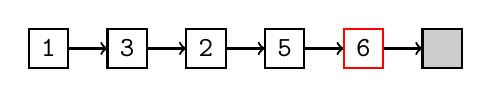
\begin{tikzpicture}
        \foreach \x[count=\i] in {1, 3, 2, 5, 6} {
            \draw[thick, ->] (\i-.5, .25) -- (\i, .25);
            \node at (\i-.75, .25) {\texttt{\x}};
        }
        \draw[thick] (0, 0) -- (0, .5) -- (.5, .5) -- (.5, 0) -- cycle;
        \draw[thick] (1, 0) -- (1, .5) -- (1.5, .5) -- (1.5, 0) -- cycle;
        \draw[thick] (2, 0) -- (2, .5) -- (2.5, .5) -- (2.5, 0) -- cycle;
        \draw[thick] (3, 0) -- (3, .5) -- (3.5, .5) -- (3.5, 0) -- cycle;
        \draw[thick, red] (4, 0) -- (4, .5) -- (4.5, .5) -- (4.5, 0) -- cycle;
        \draw[thick, fill=gray!40] (5, 0) -- (5, .5) -- (5.5, .5) -- (5.5, 0) -- cycle;
    \end{tikzpicture}
\end{center}

\subsection{Doubly Linked List}
If we want to remove a node from a linked list, then need to find the node before the removing node. The only way we can do this is by traversing the array- the function will have complexity $O(n)$. This would not be an efficient algorithm.

\noindent To make deleting an element from a linked list a constant algorithm, we introduce doubly linked lists. Here, every node has not just a \texttt{next} attribute, but also \texttt{prev}, which points to the previous node in the array. Although this makes many operations more efficient, it means we have to store more in memory.

\subsubsection{Deletion}
We now consider how to delete a node from a doubly linked list:
\begin{lstlisting}[language=pseudocode]
void delete<E>(Array<E> array, Node<E> node):
    if (node.prev != null):
        node.prev.next = node.next
    else:
        array.head = x.next
    if (node.next != null):
        node.next.prev = node.prev
\end{lstlisting}
We now visualise how the function works by deleting the node with value \texttt{4} from the doubly linked list \texttt{[1, 4, 3, 5]}:
\begin{center}
    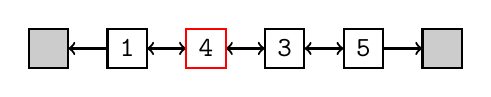
\begin{tikzpicture}
        \foreach \x[count=\i] in {1, 4, 3, 5} {
            \node at (\i-.75, .25) {\texttt{\x}};
        }
        \draw[thick, <-] (-.5, .25) -- (0, .25);
        \draw[thick, <->] (.5, .25) -- (1, .25);
        \draw[thick, <->] (1.5, .25) -- (2, .25);
        \draw[thick, <->] (2.5, .25) -- (3, .25);
        \draw[thick, ->] (3.5, .25) -- (4, .25);

        \draw[thick, fill=gray!40] (-1, 0) -- (-1, .5) -- (-.5, .5) -- (-.5, 0) -- cycle;  
        \draw[thick] (0, 0) -- (0, .5) -- (.5, .5) -- (.5, 0) -- cycle;
        \draw[thick, red] (1, 0) -- (1, .5) -- (1.5, .5) -- (1.5, 0) -- cycle;
        \draw[thick] (2, 0) -- (2, .5) -- (2.5, .5) -- (2.5, 0) -- cycle;
        \draw[thick] (3, 0) -- (3, .5) -- (3.5, .5) -- (3.5, 0) -- cycle;
        \draw[thick, fill=gray!40] (4, 0) -- (4, .5) -- (4.5, .5) -- (4.5, 0) -- cycle;
    \end{tikzpicture}
\end{center}
Since \texttt{4} isn't the \texttt{head}, we change the \texttt{next} of \texttt{1} to \texttt{3}, and the \texttt{prev} of \texttt{3} to \texttt{1}. So, the array becomes:
\begin{center}
    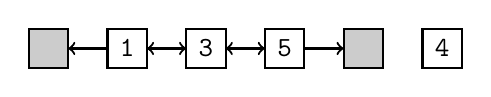
\begin{tikzpicture}
        \foreach \x[count=\i] in {1, 3, 5} {
            \node at (\i-.75, .25) {\texttt{\x}};
        }
        \node at (4.25, .25) {\texttt{4}};
        
        \draw[thick, <-] (-.5, .25) -- (0, .25);
        \draw[thick, <->] (.5, .25) -- (1, .25);
        \draw[thick, <->] (1.5, .25) -- (2, .25);
        \draw[thick, ->] (2.5, .25) -- (3, .25);

        \draw[thick, fill=gray!40] (-1, 0) -- (-1, .5) -- (-.5, .5) -- (-.5, 0) -- cycle;  
        \draw[thick] (0, 0) -- (0, .5) -- (.5, .5) -- (.5, 0) -- cycle;
        \draw[thick] (1, 0) -- (1, .5) -- (1.5, .5) -- (1.5, 0) -- cycle;
        \draw[thick] (2, 0) -- (2, .5) -- (2.5, .5) -- (2.5, 0) -- cycle;
        \draw[thick, fill=gray!40] (3, 0) -- (3, .5) -- (3.5, .5) -- (3.5, 0) -- cycle;
        \draw[thick] (4, 0) -- (4, .5) -- (4.5, .5) -- (4.5, 0) -- cycle;
    \end{tikzpicture}
\end{center}

\subsection{Circular Linked List}
Having boundary conditions complicate the operations on a (doubly) linked list. So, we connect the \texttt{head} and the \texttt{tail}. For example, the following is a circular doubly linked list:
\begin{center}
    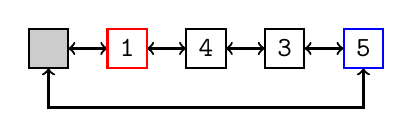
\begin{tikzpicture}
        \foreach \x[count=\i] in {1, 4, 3, 5} {
            \node at (\i-.75, .25) {\texttt{\x}};
            \draw[thick, <->] (\i-1.5, .25) -- (\i-1, .25);
        }
        
        \draw[thick, <->] (3.25, 0) -- (3.25, -.5) -- (-.75, -.5) -- (-.75, 0);
        
        \draw[thick, fill=gray!40] (-1, 0) -- (-1, .5) -- (-.5, .5) -- (-.5, 0) -- cycle;
        \draw[thick, red] (0, 0) -- (0, .5) -- (.5, .5) -- (.5, 0) -- cycle;
        \draw[thick] (1, 0) -- (1, .5) -- (1.5, .5) -- (1.5, 0) -- cycle;
        \draw[thick] (2, 0) -- (2, .5) -- (2.5, .5) -- (2.5, 0) -- cycle;
        \draw[thick, blue] (3, 0) -- (3, .5) -- (3.5, .5) -- (3.5, 0) -- cycle;
    \end{tikzpicture}
\end{center}
\noindent The first element is called the sentinel \texttt{gap}, and has no value- the element before the sentinel is the \texttt{tail} (boxed in blue), while the element after the sentinel is the \texttt{head} (boxed in red). Using the circular doubly linked with a sentinel, the functions we covered have much fewer conditions. The three functions \texttt{delete}, \texttt{insert} and \texttt{search} are listed below:
\begin{lstlisting}[language=pseudocode]
// delete the specified node from the array
void delete<E>(CLinkedArray<E> array, Node<E> node):
    node.prev.next = node.next
    node.next.prev = node.prev
\end{lstlisting}
\begin{lstlisting}[language=pseudocode]
// add to the head of the array
void insert<E>(CLinkedArray<E> array, Node<E> node):
    node.next = array.head
    array.head.prev = node
    array.head = node
    node.prev = gap
\end{lstlisting}
\begin{lstlisting}[language=pseudocode]
// find the node in the array with that value
Node<E> search<E>(CLinkedArray<E> array, E value):
    Node<E> node = array.head
    // search until we find the element or we end up at the gap
    while (node != gap && node.value != value):
        node = node.next
    return node
\end{lstlisting}
\newpage

\section{Abstract Data Types}
An abstract data type (ADT) defines a data type and operations on the data type. For example, for the data type array, we expect indexing every element. An ADT is a class of objects whose logical behaviour is defined by a set of values and operations- it is an abstract expectation of the implementation. We make use of data structures to make a concrete implementation of the data type. The ADT is the logic, while the data structure makes it physical.

\subsection{Stack}
The stack ADT stores elements. It allows us to add and delete elements using the last-in-first-out (LIFO) policy. The main operations defined on a stack are:
\begin{itemize}
    \item \texttt{void push<E>(Stack<E> stack, E element)}, which adds the \texttt{element} into the stack;
    \item \texttt{E pop<E>(Stack<E> stack)}, which removes and returns the most recently pushed element from the stack.
\end{itemize}
Along with these operations, we also have the following additional operations:
\begin{itemize}
    \item \texttt{E peek<E>(Stack<E> stack)}, which returns the most recently pushed element from the stack without removing it;
    \item \texttt{int size<E>(Stack<E> stack)}, which returns the number of elements in the stack;
    \item \texttt{boolean isEmpty<E>(Stack<E> stack)}, which returns \texttt{true} if the stack is empty, and \texttt{false} otherwise.
\end{itemize}
Now, we see how we can perform the operations on the stack. We first push the element \texttt{2} into the stack. Then, the stack becomes:
\begin{center}
    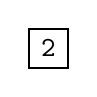
\begin{tikzpicture}
        \foreach \x[count=\i] in {2} {
            \draw[thick] (\i, 0) -- (\i+.5, 0) -- (\i+.5, .5) -- (\i, .5) -- cycle;
            \node at (\i+.25, .25) {\texttt{\x}};
        }
    \end{tikzpicture}
\end{center}
Then, we push \texttt{3} onto the stack. The stack is now
\begin{center}
    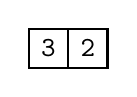
\begin{tikzpicture}
        \foreach \x[count=\i] in {3, 2} {
            \draw[thick] (\i*1/2, 0) -- (\i*1/2+.5, 0) -- (\i*1/2+.5, .5) -- (\i*1/2, .5) -- cycle;
            \node at (\i*1/2+.25, .25) {\texttt{\x}};
        }
    \end{tikzpicture}
\end{center}
We represent pushing an element as adding to the left. It can be represented in any of the other 3 possibilities as well. Now, we push \texttt{5} to the stack. Now, the stack is
\begin{center}
    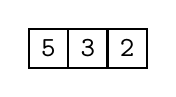
\begin{tikzpicture}
        \foreach \x[count=\i] in {5, 3, 2} {
            \draw[thick] (\i*1/2, 0) -- (\i*1/2+.5, 0) -- (\i*1/2+.5, .5) -- (\i*1/2, .5) -- cycle;
            \node at (\i*1/2+.25, .25) {\texttt{\x}};
        }
    \end{tikzpicture}
\end{center}
If we now pop the stack, we get the value \texttt{5} out of the stack. Also, the stack is now
\begin{center}
    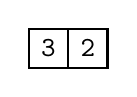
\begin{tikzpicture}
        \foreach \x[count=\i] in {3, 2} {
            \draw[thick] (\i*1/2, 0) -- (\i*1/2+.5, 0) -- (\i*1/2+.5, .5) -- (\i*1/2, .5) -- cycle;
            \node at (\i*1/2+.25, .25) {\texttt{\x}};
        }
    \end{tikzpicture}
\end{center}
Now, we peek the stack- we get the value \texttt{3}, but the stack remains unchanged. Next, we pop again. We return \texttt{3} by the operation, making the stack
\begin{center}
    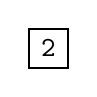
\begin{tikzpicture}
        \foreach \x[count=\i] in {2} {
            \draw[thick] (\i*1/2, 0) -- (\i*1/2+.5, 0) -- (\i*1/2+.5, .5) -- (\i*1/2, .5) -- cycle;
            \node at (\i*1/2+.25, .25) {\texttt{\x}};
        }
    \end{tikzpicture}
\end{center}
Finally, we push \texttt{7} into the stack. The final state of the stack is
\begin{center}
    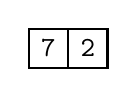
\begin{tikzpicture}
        \foreach \x[count=\i] in {7, 2} {
            \draw[thick] (\i*1/2, 0) -- (\i*1/2+.5, 0) -- (\i*1/2+.5, .5) -- (\i*1/2, .5) -- cycle;
            \node at (\i*1/2+.25, .25) {\texttt{\x}};
        }
    \end{tikzpicture}
\end{center}

\subsubsection{Array implementation}
Now, we consider implementations of the stack using an array. Since an array can only be of a particular size, the size of the stack is also limited. In fact, if the array is of length \texttt{n}, then the size of the stack is \texttt{n}. We keep track of the index \texttt{top} to keep track of the top value of the stack.

\noindent We cannot pop from an empty stack. This is true for all stacks. On the other hand, using an array implementation, we also cannot push to a full stack. This is not part of the logic of a stack. 

\noindent Keeping track of the \texttt{top} element within the array, the following is the pseudocode for the stack:
\begin{lstlisting}[language=pseudocode]
boolean isEmpty<E>(Stack<E> stack):
    return stack.top == -1
\end{lstlisting}

\begin{lstlisting}[language=pseudocode]
void push<E>(Stack<E> stack, E value):
    stack.top++
    stack.array[stack.top] = value
\end{lstlisting}

\begin{lstlisting}[language=pseudocode]
E pop(Stack<E> stack):
    if (stack.isEmpty):
        throw UnderflowError
    stack.top--
    return stack.array[stack.top+1]
\end{lstlisting}
We show how the concrete implementation handles the stack operations we discussed above. We start with an array of size 5.
\begin{center}
    \begin{tikzpicture}
        \foreach \x in {0, 1, 2, 3, 4} {
            \draw[thick] (\x*1/2-.1, 0) -- (\x*1/2+.1, 0);
        }
        \draw[thick, blue] (-.25, 0) -- (-.25, .5);
    \end{tikzpicture}
\end{center}
To the left of the blue wall, we have the element \texttt{top}- it is initialised with value \texttt{-1}. We then push \texttt{2} onto the stack:
\begin{center}
    \begin{tikzpicture}
        \foreach \x in {0, 1, 2, 3, 4} {
            \draw[thick] (\x*1/2-.1, 0) -- (\x*1/2+.1, 0);
        }
        \node at (0, .25) {\texttt{2}};
        \draw[thick, blue] (.25, 0) -- (.25, .5);
    \end{tikzpicture}
\end{center}
Adding an element increments the value of \texttt{top}. Next, we push \texttt{3} onto the stack:
\begin{center}
    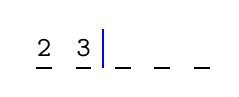
\begin{tikzpicture}
        \foreach \x in {0, 1, 2, 3, 4} {
            \draw[thick] (\x*1/2-.1, 0) -- (\x*1/2+.1, 0);
        }
        \node at (0, .25) {\texttt{2}};
        \node at (.5, .25) {\texttt{3}};
        \draw[thick, blue] (.75, 0) -- (.75, .5);
    \end{tikzpicture}
\end{center}
We push \texttt{5} onto the stack now:
\begin{center}
    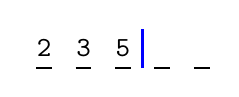
\begin{tikzpicture}
        \foreach \x in {0, 1, 2, 3, 4} {
            \draw[thick] (\x*1/2-.1, 0) -- (\x*1/2+.1, 0);
        }
        \node at (0, .25) {\texttt{2}};
        \node at (.5, .25) {\texttt{3}};
        \node at (1, .25) {\texttt{5}};
        \draw[thick, blue] (1.25, 0) -- (1.25, .5);
    \end{tikzpicture}
\end{center}
Now, we wish to pop the stack. So, we return \texttt{5}, and the stack becomes
\begin{center}
    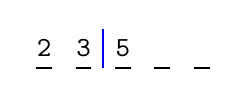
\begin{tikzpicture}
        \foreach \x in {0, 1, 2, 3, 4} {
            \draw[thick] (\x*1/2-.1, 0) -- (\x*1/2+.1, 0);
        }
        \node at (0, .25) {\texttt{2}};
        \node at (.5, .25) {\texttt{3}};
        \node at (1, .25) {\texttt{5}};
        \draw[thick, blue] (.75, 0) -- (.75, .5);
    \end{tikzpicture}
\end{center}
Although \texttt{5} is still in the array, it doesn't matter since \texttt{top} has been decremented- it gets overridden when we push again. Next, we peek the stack- this returns \texttt{3}, and the stack remains unchanged. Then, we pop the stack. This returns \texttt{3} as well, but the stack changes this time. It is now
\begin{center}
    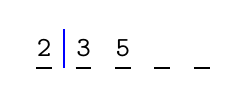
\begin{tikzpicture}
        \foreach \x in {0, 1, 2, 3, 4} {
            \draw[thick] (\x*1/2-.1, 0) -- (\x*1/2+.1, 0);
        }
        \node at (0, .25) {\texttt{2}};
        \node at (.5, .25) {\texttt{3}};
        \node at (1, .25) {\texttt{5}};
        \draw[thick, blue] (.25, 0) -- (.25, .5);
    \end{tikzpicture}
\end{center}
Finally, we push \texttt{7} onto the stack
\begin{center}
    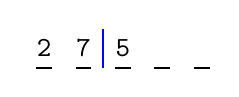
\begin{tikzpicture}
        \foreach \x in {0, 1, 2, 3, 4} {
            \draw[thick] (\x*1/2-.1, 0) -- (\x*1/2+.1, 0);
        }
        \node at (0, .25) {\texttt{2}};
        \node at (.5, .25) {\texttt{7}};
        \node at (1, .25) {\texttt{5}};
        \draw[thick, blue] (.75, 0) -- (.75, .5);
    \end{tikzpicture}
\end{center}
So, \texttt{3} gets overridden with \texttt{7}.

\noindent All the operations in the array run in constant time. The space used is always $O(n)$, where $n$ is the size of the array. So, $n$ can be much larger than the size of the stack. Also, $n$ must be known at the start.

\noindent To overcome these issues, we make use of a resizable array. Here, if we have an overflow, we increase the size of the array. Similarly, if most of the array isn't being used, we decrease the size of the array. We now avoid overflow errors. Expanding the array takes $O(n)$ time overall. 

\noindent We now consider the pseudocode for \texttt{resize}.
\begin{lstlisting}[language=pseudocode]
void resize<E>(Stack<E> stack, int newLength):
    // newArray has size newLength
    Array<E> newArray = []
    for (int i = 0; i < stack.top; i++):
        newArray[i] = stack.array[i]
    stack.array = newArray
\end{lstlisting}
Here, we copy all the values from the \texttt{array} in the \texttt{stack} onto the \texttt{newArray}, and then make that array the array of the \texttt{stack}. We now look at how this function is called from the implementations of \texttt{pop} and \texttt{push}.
\begin{lstlisting}[language=pseudocode]
E pop<E>(Stack<E> stack):
    if (stack.isEmpty):
        throw UnderflowError
    E value = stack.array[stack.top]
    stack.top--
    // half the array if only a quarter of it is being used
    if (stack.top > 0 && stack.top == n/4):
        resize(stack, n/2)
\end{lstlisting}
\begin{lstlisting}[language=pseudocode]
void push<E>(Stack<E> stack, E value):
    // if not enough space, double the array
    if (stack.top == n-1):
        resize(stack, 2*n)
    stack.top++
    stack.array[stack.top] = value
\end{lstlisting}
For example, if we had the stack
\begin{center}
    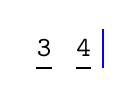
\begin{tikzpicture}
        \foreach \x in {0, 1} {
            \draw[thick] (\x*1/2-.1, 0) -- (\x*1/2+.1, 0);
        }
        \node at (0, .25) {\texttt{3}};
        \node at (.5, .25) {\texttt{4}};
        \draw[thick, blue] (.75, 0) -- (.75, .5);
    \end{tikzpicture}
\end{center}
and we wanted to push \texttt{5}, the stack then becomes
\begin{center}
    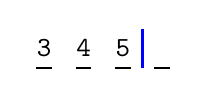
\begin{tikzpicture}
        \foreach \x in {0, 1, 2, 3} {
            \draw[thick] (\x*1/2-.1, 0) -- (\x*1/2+.1, 0);
        }
        \node at (0, .25) {\texttt{3}};
        \node at (.5, .25) {\texttt{4}};
        \node at (1, .25) {\texttt{5}};
        \draw[thick, blue] (1.25, 0) -- (1.25, .5);
    \end{tikzpicture}
\end{center}
If we now pop twice, then we end up with
\begin{center}
    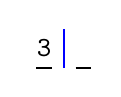
\begin{tikzpicture}
        \foreach \x in {0, 1} {
            \draw[thick] (\x*1/2-.1, 0) -- (\x*1/2+.1, 0);
        }
        \node at (0, .25) {\texttt{3}};
        \draw[thick, blue] (.25, 0) -- (.25, .5);
    \end{tikzpicture}
\end{center}
When consider the running time of a resizable array implementation, we perform amortised analysis. That is, we consider the average case. For instance, if we want to add \texttt{n+1} push operations to the stack, then the first \texttt{n} operations are $O(1)$, while the last one is $O(n)$ since we need to resize. On average, this means that the running time is $O(1)$. Therefore, the amortised running time of the push operation is $O(1)$.

\subsubsection{Linked list implementation}
\noindent Now, we consider the linked list implementation. A linked list follows LIFO policy when adding and removing, so it is the same implementation. In particular, the \texttt{top} of a stack is the \texttt{head} of a linked list. Moreover, all the operations are constant- we can keep track of the \texttt{size} attribute in order to make it run in constant time.

\subsection{Queue}
Like a stack, the queue ADT also stores arbitrary elements. However, the insertions and deletions obey first-in-first-out (FIFO) policy. The main operations on a queue are:
\begin{itemize}
    \item \texttt{void enqueue<E>(Queue<E> queue, E value)}, which inserts \texttt{value} at the end of the \texttt{queue};
    \item \texttt{E dequeue<E>(Queue<E> queue)}, which removes and returns the element at the head of the \texttt{queue}.
\end{itemize}
Other operations defined on a queue are:
\begin{itemize}
    \item \texttt{E front<E>(Queue<E> queue)}, which returns the element at the head of the \texttt{queue} without removing it;
    \item \texttt{int size<E>(Queue<E> queue)}, which returns the number of elements in the \texttt{queue};
    \item \texttt{boolean isEmpty<E>(Queue<E> queue)}, which returns \texttt{true} if there are no elements in the \texttt{queue} and \texttt{false} if there are elements in the \texttt{queue}.
\end{itemize}
We describe how we these operations apply to the queue. First, to an empty queue, we add \texttt{5}.
\begin{center}
    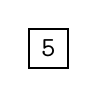
\begin{tikzpicture}
        \foreach \x[count=\i] in {5} {
            \draw[thick] (\i*1/2, 0) -- (\i*1/2+.5, 0) -- (\i*1/2+.5, .5) -- (\i*1/2, .5) -- cycle;
            \node at (\i*1/2+.25, .25) {\texttt{\x}};
        }
    \end{tikzpicture}
\end{center}
Next, we add \texttt{3} to the queue:
\begin{center}
    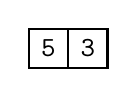
\begin{tikzpicture}
        \foreach \x[count=\i] in {5, 3} {
            \draw[thick] (\i*1/2, 0) -- (\i*1/2+.5, 0) -- (\i*1/2+.5, .5) -- (\i*1/2, .5) -- cycle;
            \node at (\i*1/2+.25, .25) {\texttt{\x}};
        }
    \end{tikzpicture}
\end{center}
We set the leftmost element of the queue the front, while the rightmost element of the queue the back. This is why \texttt{3} gets place to the right of \texttt{5}. Now, we add \texttt{7} to the queue.
\begin{center}
    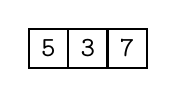
\begin{tikzpicture}
        \foreach \x[count=\i] in {5, 3, 7} {
            \draw[thick] (\i*1/2, 0) -- (\i*1/2+.5, 0) -- (\i*1/2+.5, .5) -- (\i*1/2, .5) -- cycle;
            \node at (\i*1/2+.25, .25) {\texttt{\x}};
        }
    \end{tikzpicture}
\end{center}
Now, we dequeue the queue. So, we return \texttt{5} and the queue becomes
\begin{center}
    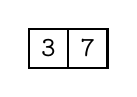
\begin{tikzpicture}
        \foreach \x[count=\i] in {3, 7} {
            \draw[thick] (\i*1/2, 0) -- (\i*1/2+.5, 0) -- (\i*1/2+.5, .5) -- (\i*1/2, .5) -- cycle;
            \node at (\i*1/2+.25, .25) {\texttt{\x}};
        }
    \end{tikzpicture}
\end{center}
We dequeue again, returning \texttt{3}. The queue is now
\begin{center}
    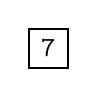
\begin{tikzpicture}
        \foreach \x[count=\i] in {7} {
            \draw[thick] (\i*1/2, 0) -- (\i*1/2+.5, 0) -- (\i*1/2+.5, .5) -- (\i*1/2, .5) -- cycle;
            \node at (\i*1/2+.25, .25) {\texttt{\x}};
        }
    \end{tikzpicture}
\end{center}
If we peek at the \texttt{front} of the queue, we return \texttt{7}, but the queue remains unchanged. If we dequeue, then \texttt{7} gets returned, and the queue is empty. Trying to dequeue again raises an error. If we check \texttt{isEmpty}, we will get back \texttt{true}.

\subsubsection{Array implementation}
Now, we look at the array implementation of a queue. Due to the nature of an array, the queue has a capacity. The array implementation makes use of two attributes- \texttt{head} and \texttt{tail} that track the indices of the head and the tail of the queue respectively. The value of \texttt{tail} is one further than the actual index of \texttt{tail}- it points to the location where the next element will be added. For example, the following is a possible queue:
\begin{center}
    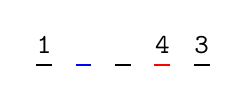
\begin{tikzpicture}
        \draw[thick] (-.1, 0) -- (.1, 0);
        \draw[thick, blue] (.4, 0) -- (.6, 0);
        \draw[thick] (.9, 0) -- (1.1, 0);
        \draw[thick, red] (1.4, 0) -- (1.6, 0);
        \draw[thick] (1.9, 0) -- (2.1, 0);
        \node at (0, .25) {\texttt{1}};
        \node at (1.5, .25) {\texttt{4}};
        \node at (2, .25) {\texttt{3}};
    \end{tikzpicture}
\end{center}
The blue spot is the location of \texttt{tail}, while the red spot marks the \texttt{head} of the queue. So, the \texttt{tail} is always empty- an array of length \texttt{n} implements a queue with maximum length \texttt{n-1}. Moreover, the queue is empty if and only if the \texttt{head} and the \texttt{tail} indices match.

\noindent The operations on the array implementation increment the values of \texttt{head} and \texttt{tail} in a circular manner (i.e. modular addition). We now consider the operations:
\begin{lstlisting}[language=pseudocode]
boolean isEmpty<E>(Queue<E> queue):
    return queue.head == queue.tail
\end{lstlisting}

\begin{lstlisting}[language=pseudocode]
int size<E>(Queue<E> queue):
    return (queue.array.length - queue.head + queue.tail) % queue.array.length
\end{lstlisting}

\begin{lstlisting}[language=pseudocode]
void enqueue<E>(Queue<E> queue, E value):
    if (queue.size == n-1):
        throw OverflowError
    queue.array[queue.tail] = value
    queue.tail = (queue.tail + 1) % queue.array.length
\end{lstlisting}

\begin{lstlisting}[language=pseudocode]
E dequeue<E>(Queue<E> queue):
    if (queue.isEmpty):
        throw UnderflowError
    E value = queue.array[queue.head]
    queue.head = (queue.head + 1) & queue.array.length
    return value
\end{lstlisting}
We consider these operations using the array
\begin{center}
    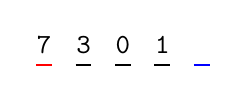
\begin{tikzpicture}
        \draw[thick, red] (-.1, 0) -- (.1, 0);
        \draw[thick] (.4, 0) -- (.6, 0);
        \draw[thick] (.9, 0) -- (1.1, 0);
        \draw[thick] (1.4, 0) -- (1.6, 0);
        \draw[thick, blue] (1.9, 0) -- (2.1, 0);
        \node at (0, .25) {\texttt{7}};
        \node at (.5, .25) {\texttt{3}};
        \node at (1, .25) {\texttt{0}};
        \node at (1.5, .25) {\texttt{1}};
    \end{tikzpicture}
\end{center}
The queue is full. We dequeue, which returns \texttt{7}, and increments the value of \texttt{head} modulo \texttt{5}.
\begin{center}
    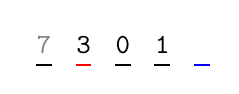
\begin{tikzpicture}
        \draw[thick] (-.1, 0) -- (.1, 0);
        \draw[thick, red] (.4, 0) -- (.6, 0);
        \draw[thick] (.9, 0) -- (1.1, 0);
        \draw[thick] (1.4, 0) -- (1.6, 0);
        \draw[thick, blue] (1.9, 0) -- (2.1, 0);
        \node[gray] at (0, .25) {\texttt{7}};
        \node at (.5, .25) {\texttt{3}};
        \node at (1, .25) {\texttt{0}};
        \node at (1.5, .25) {\texttt{1}};
    \end{tikzpicture}
\end{center}
Note that the value \texttt{7} is still in the array. This doesn't matter since the \texttt{head} points to the next element \texttt{3}. Now, we enqueue \texttt{4}. This increments the value of \texttt{tail} modulo \texttt{5}.
\begin{center}
    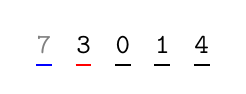
\begin{tikzpicture}
        \draw[thick, blue] (-.1, 0) -- (.1, 0);
        \draw[thick, red] (.4, 0) -- (.6, 0);
        \draw[thick] (.9, 0) -- (1.1, 0);
        \draw[thick] (1.4, 0) -- (1.6, 0);
        \draw[thick] (1.9, 0) -- (2.1, 0);
        \node[gray] at (0, .25) {\texttt{7}};
        \node at (.5, .25) {\texttt{3}};
        \node at (1, .25) {\texttt{0}};
        \node at (1.5, .25) {\texttt{1}};
        \node at (2, .25) {\texttt{4}};
    \end{tikzpicture}
\end{center}
Since \texttt{4+1=5}, the value of \texttt{tail} becomes \texttt{0}. We now compute the \texttt{size} of the array, which is \texttt{5-1+0=4} modulo \texttt{5}, so \texttt{4}. Next, we dequeue.
\begin{center}
    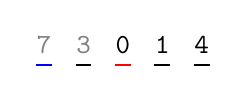
\begin{tikzpicture}
        \draw[thick, blue] (-.1, 0) -- (.1, 0);
        \draw[thick] (.4, 0) -- (.6, 0);
        \draw[thick, red] (.9, 0) -- (1.1, 0);
        \draw[thick] (1.4, 0) -- (1.6, 0);
        \draw[thick] (1.9, 0) -- (2.1, 0);
        \node[gray] at (0, .25) {\texttt{7}};
        \node[gray] at (.5, .25) {\texttt{3}};
        \node at (1, .25) {\texttt{0}};
        \node at (1.5, .25) {\texttt{1}};
        \node at (2, .25) {\texttt{4}};
    \end{tikzpicture}
\end{center}
We dequeue again.
\begin{center}
    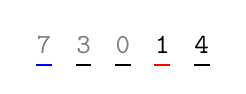
\begin{tikzpicture}
        \draw[thick, blue] (-.1, 0) -- (.1, 0);
        \draw[thick] (.4, 0) -- (.6, 0);
        \draw[thick] (.9, 0) -- (1.1, 0);
        \draw[thick, red] (1.4, 0) -- (1.6, 0);
        \draw[thick] (1.9, 0) -- (2.1, 0);
        \node[gray] at (0, .25) {\texttt{7}};
        \node[gray] at (.5, .25) {\texttt{3}};
        \node[gray] at (1, .25) {\texttt{0}};
        \node at (1.5, .25) {\texttt{1}};
        \node at (2, .25) {\texttt{4}};
    \end{tikzpicture}
\end{center}
Finally, we enqueue \texttt{5}.
\begin{center}
    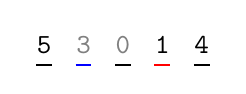
\begin{tikzpicture}
        \draw[thick] (-.1, 0) -- (.1, 0);
        \draw[thick, blue] (.4, 0) -- (.6, 0);
        \draw[thick] (.9, 0) -- (1.1, 0);
        \draw[thick, red] (1.4, 0) -- (1.6, 0);
        \draw[thick] (1.9, 0) -- (2.1, 0);
        \node at (0, .25) {\texttt{5}};
        \node[gray] at (.5, .25) {\texttt{3}};
        \node[gray] at (1, .25) {\texttt{0}};
        \node at (1.5, .25) {\texttt{1}};
        \node at (2, .25) {\texttt{4}};
    \end{tikzpicture}
\end{center}
The space used is always $O(n)$, where $n$ is the length of the array. So, we might be wasting space. Nonetheless, while the operations are $O(1)$. To counter the waste of space, we can make use of a resizable size implementation, the same way we used in stack. Then, all the operations take amortised constant time. The resize function is shown below:
\begin{lstlisting}[language=pseudocode]
void resize<E>(Stack<E> stack, int newLength):
    // array has length newLength
    Array<E> array = []
    for (int i = 0; i < n-1; i++):
        array[i] = queue.array[(queue.head+i) % queue.array.length]
    queue.tail = queue.array.length
    queue.array = array
    queue.head = 0
\end{lstlisting}
When we resize, we place the elements in the array from \texttt{0} to \texttt{n-2}. We make use of the resize operation when performing the operations enqueue and dequeue, either halfing or doubling the length of the array.

\subsubsection{Linked list implementation}
Now, we consider the linked list implementation. The linked list we use here has a tail pointer for efficiency. Then, the \texttt{head} and the \texttt{tail} of the list and the stack match. Moreover, \texttt{enqueue} is implemented by adding to the tail, while \texttt{dequeue} is implemented by removing from the head. All the operations are performed in constant time, except for computing the \texttt{size}. But, keeping track of the \texttt{size} will make it a constant operation. Moreover, there are no overflows since the linked list implementation is dynamic.

\noindent Using doubly linked list has the same performance, but is less memory efficient.

\subsection{Dequeue}
The doubly ended queue (dequeue) ADT supports insertion and deletion from both ends. The operations here are:
\begin{itemize}
    \item \texttt{void pushBack<E>(Dequeue<E> dequeue, E value)}, which inserts the \texttt{value} at the end of the dequeue;
    \item \texttt{void pushFront<E>(Dequeue<E> dequeue, E value)}, which inserts the \texttt{value} at the start of the dequeue;
    \item \texttt{E popBack<E>(Dequeue<E> dequeue)}, which pops the element from the end of the queue.
    \item \texttt{E popFront<E>(Dequeue<E> dequeue)}, which pops the element from the start of the queue.
\end{itemize}
Other operations defined on a dequeue are:
\begin{itemize}
    \item \texttt{E front<E>(Dequeue<E> dequeue)}, which returns the element at the head of the queue without removing it;
    \item \texttt{E back<E>(Dequeue<E> dequeue)}, which returns the element at the back of the queue without removing it;
    \item \texttt{int size<E>(Dequeue<E> dequeue)}, which returns the number of elements in the \texttt{dequeue};
    \item \texttt{boolean isEmpty<E>(Dequeue<E> dequeue)}, which returns \texttt{true} if there are no elements in the \texttt{dequeue} and \texttt{false} if there are elements in the \texttt{dequeue}.
\end{itemize}
We describe how we these operations apply to the dequeue. First, to an empty dequeue, we push \texttt{1} to the front.
\begin{center}
    \begin{tikzpicture}
        \foreach \x[count=\i] in {1} {
            \draw[thick] (\i*1/2, 0) -- (\i*1/2+.5, 0) -- (\i*1/2+.5, .5) -- (\i*1/2, .5) -- cycle;
            \node at (\i*1/2+.25, .25) {\texttt{\x}};
        }
    \end{tikzpicture}
\end{center}
Now, we push \texttt{3} to the back of the dequeue.
\begin{center}
    \begin{tikzpicture}
        \foreach \x[count=\i] in {1, 3} {
            \draw[thick] (\i*1/2, 0) -- (\i*1/2+.5, 0) -- (\i*1/2+.5, .5) -- (\i*1/2, .5) -- cycle;
            \node at (\i*1/2+.25, .25) {\texttt{\x}};
        }
    \end{tikzpicture}
\end{center}
Next, we push \texttt{5} to the front of the dequeue. 
\begin{center}
    \begin{tikzpicture}
        \foreach \x[count=\i] in {5, 1, 3} {
            \draw[thick] (\i*1/2, 0) -- (\i*1/2+.5, 0) -- (\i*1/2+.5, .5) -- (\i*1/2, .5) -- cycle;
            \node at (\i*1/2+.25, .25) {\texttt{\x}};
        }
    \end{tikzpicture}
\end{center}
If we calculate the \texttt{size} of the dequeue, we get \texttt{3}. Then, we pop back the dequeue. This returns \texttt{3}, and the dequeue becomes
\begin{center}
    \begin{tikzpicture}
        \foreach \x[count=\i] in {5, 1} {
            \draw[thick] (\i*1/2, 0) -- (\i*1/2+.5, 0) -- (\i*1/2+.5, .5) -- (\i*1/2, .5) -- cycle;
            \node at (\i*1/2+.25, .25) {\texttt{\x}};
        }
    \end{tikzpicture}
\end{center}
We now push \texttt{0} to the front of the dequeue.
\begin{center}
    \begin{tikzpicture}
        \foreach \x[count=\i] in {0, 5, 1} {
            \draw[thick] (\i*1/2, 0) -- (\i*1/2+.5, 0) -- (\i*1/2+.5, .5) -- (\i*1/2, .5) -- cycle;
            \node at (\i*1/2+.25, .25) {\texttt{\x}};
        }
    \end{tikzpicture}
\end{center}
The \texttt{front} of the dequeue is \texttt{0}, while the \texttt{back} of the deque is \texttt{1}. Finally, we pop front the dequeue. This return \texttt{0}, and the dequeue becomes
\begin{center}
    \begin{tikzpicture}
        \foreach \x[count=\i] in {5, 1} {
            \draw[thick] (\i*1/2, 0) -- (\i*1/2+.5, 0) -- (\i*1/2+.5, .5) -- (\i*1/2, .5) -- cycle;
            \node at (\i*1/2+.25, .25) {\texttt{\x}};
        }
    \end{tikzpicture}
\end{center}

\subsubsection{Array implementation}
We now consider the array implementation of a dequeue. This is very similar to the array implementation of queue, just with a few further functions. One of the most important differences is that when we add to an empty dequeue or remove to get an empty dequeue, pushing and popping from the front is the same as doing the operations from the back. The code is shown below:
\begin{lstlisting}[language=pseudocode]
void pushBack<E>(Dequeue<E> dequeue, E value):
    if (dequeue.size == n-1):
        throw OverflowError
    dequeue.array[dequeue.tail] = value
    dequeue.tail = (dequeue.tail+1) % dequeue.array.length
\end{lstlisting}
\begin{lstlisting}[language=pseudocode]
void pushFront<E>(Dequeue<E> dequeue, E value):
    if (dequeue.size == n-1):
        throw OverflowError
    // if list empty, add to the tail
    if (dequeue.head == dequeue.tail):
        dequeue.array[dequeue.tail] = value
        dequeue.tail = (dequeue.tail+1) % dequeue.array.length
    // otherwise add to the front
    else:
        dequeue.head = (dequeue.head-1) % dequeue.array.length
        dequeue.array[dequeue.head] = value
\end{lstlisting}
\begin{lstlisting}[language=pseudocode]
E popBack<E>(Dequeue<E> dequeue):
    if (dequeue.isEmpty):
        throw UnderflowError
    dequeue.tail = (dequeue.tail-1) % dequeue.array.length
    return dequeue.array[dequeue.tail]
\end{lstlisting}
\begin{lstlisting}[language=pseudocode]
E popFront<E>(Dequeue<E> dequeue):
    if (dequeue.isEmpty):
        throw UnderflowError
    // if this is the only element, then pop back not pop front
    if (head+1 == tail):
        dequeue.tail = (dequeue.tail-1) % dequeue.array.length
        return dequeue.array[dequeue.tail]
    else:
        E value = dequeue.array[dequeue.head]
        dequeue.head = (dequeue.head+1) % dequeue.array.length
        return value
\end{lstlisting}
\begin{lstlisting}[language=pseudocode]
int size<E>(Dequeue<E> dequeue):
    return (dequeue.array.length - dequeue.head + dequeue.tail) % dequeue.array.length
\end{lstlisting}
All the operations not shown are the same as a queue. We consider these operations using the array
\begin{center}
    \begin{tikzpicture}
        \draw[thick] (-.1, 0) -- (.1, 0);
        \draw[thick] (.4, 0) -- (.6, 0);
        \draw[thick, blue] (.9, 0) -- (1.1, 0);
        \draw[thick] (1.4, 0) -- (1.6, 0);
        \draw[thick] (1.9, 0) -- (2.1, 0);
        \draw[thick, red] (2.4, 0) -- (2.6, 0);
        \node at (0, .25) {\texttt{1}};
        \node at (.5, .25) {\texttt{3}};
        \node at (2.5, .25) {\texttt{1}};
    \end{tikzpicture}
\end{center}
The head here is \texttt{1}, while the tail is \texttt{3}- we traverse rightwards in a circular fashion. This is similar to the array implemented by queue. First, we push \texttt{2} to the tail of the dequeue.
\begin{center}
    \begin{tikzpicture}
        \draw[thick] (-.1, 0) -- (.1, 0);
        \draw[thick] (.4, 0) -- (.6, 0);
        \draw[thick] (.9, 0) -- (1.1, 0);
        \draw[thick, blue] (1.4, 0) -- (1.6, 0);
        \draw[thick] (1.9, 0) -- (2.1, 0);
        \draw[thick, red] (2.4, 0) -- (2.6, 0);
        \node at (0, .25) {\texttt{1}};
        \node at (.5, .25) {\texttt{3}};
        \node at (1, .25) {\texttt{2}};
        \node at (2.5, .25) {\texttt{1}};
    \end{tikzpicture}
\end{center}
Pushing to the end implies incrementing the \texttt{tail} in a circular fashion. Moreover, we add the element to the right, to where the \texttt{tail} was. Next, we push \texttt{0} to the front.
\begin{center}
    \begin{tikzpicture}
        \draw[thick] (-.1, 0) -- (.1, 0);
        \draw[thick] (.4, 0) -- (.6, 0);
        \draw[thick] (.9, 0) -- (1.1, 0);
        \draw[thick, blue] (1.4, 0) -- (1.6, 0);
        \draw[thick, red] (1.9, 0) -- (2.1, 0);
        \draw[thick] (2.4, 0) -- (2.6, 0);
        \node at (0, .25) {\texttt{1}};
        \node at (.5, .25) {\texttt{3}};
        \node at (1, .25) {\texttt{2}};
        \node at (2, .25) {\texttt{0}};
        \node at (2.5, .25) {\texttt{1}};
    \end{tikzpicture}
\end{center}
Pushing to the front implies decrementing the \texttt{head} in a circular fashion. Moreover, we add the element to the left, the index after the \texttt{head}. Now, we pop from the front of the dequeue. This returns \texttt{0}, and the array becomes
\begin{center}
    \begin{tikzpicture}
        \draw[thick] (-.1, 0) -- (.1, 0);
        \draw[thick] (.4, 0) -- (.6, 0);
        \draw[thick] (.9, 0) -- (1.1, 0);
        \draw[thick, blue] (1.4, 0) -- (1.6, 0);
        \draw[thick] (1.9, 0) -- (2.1, 0);
        \draw[thick, red] (2.4, 0) -- (2.6, 0);
        \node at (0, .25) {\texttt{1}};
        \node at (.5, .25) {\texttt{3}};
        \node at (1, .25) {\texttt{2}};
        \node[gray] at (2, .25) {\texttt{0}};
        \node at (2.5, .25) {\texttt{1}};
    \end{tikzpicture}
\end{center}
Like with the queue, the element isn't removed- we just increment \texttt{head} in a circular fashion. The \texttt{front} of the dequeue is \texttt{1}, and the \texttt{tail} is \texttt{2}. Then, we push \texttt{3} to the front.
\begin{center}
    \begin{tikzpicture}
        \draw[thick] (-.1, 0) -- (.1, 0);
        \draw[thick] (.4, 0) -- (.6, 0);
        \draw[thick] (.9, 0) -- (1.1, 0);
        \draw[thick, blue] (1.4, 0) -- (1.6, 0);
        \draw[thick, red] (1.9, 0) -- (2.1, 0);
        \draw[thick] (2.4, 0) -- (2.6, 0);
        \node at (0, .25) {\texttt{1}};
        \node at (.5, .25) {\texttt{3}};
        \node at (1, .25) {\texttt{2}};
        \node at (2, .25) {\texttt{3}};
        \node at (2.5, .25) {\texttt{1}};
    \end{tikzpicture}
\end{center}
This decrements the \texttt{head} in a circular fashion, and replaces the \texttt{0} with \texttt{3}. Finally, we pop back from the dequeue. This returns \texttt{2}, and the dequeue becomes
\begin{center}
    \begin{tikzpicture}
        \draw[thick] (-.1, 0) -- (.1, 0);
        \draw[thick] (.4, 0) -- (.6, 0);
        \draw[thick, blue] (.9, 0) -- (1.1, 0);
        \draw[thick] (1.4, 0) -- (1.6, 0);
        \draw[thick, red] (1.9, 0) -- (2.1, 0);
        \draw[thick] (2.4, 0) -- (2.6, 0);
        \node at (0, .25) {\texttt{1}};
        \node at (.5, .25) {\texttt{3}};
        \node[gray] at (1, .25) {\texttt{2}};
        \node at (2, .25) {\texttt{3}};
        \node at (2.5, .25) {\texttt{1}};
    \end{tikzpicture}
\end{center}
Now, the \texttt{head} and the \texttt{tail} of the dequeue is \texttt{3}. The \texttt{size} is now \texttt{4}.

\noindent To overcome the size limitation of the dequeue, we can make use of a resizable array implementation, like in the case of a queue. All the operations, in both cases, takes (amortised) constant running time.

\subsubsection{Doubly linked list implementation}
We can implement a dequeue using a doubly linked list with a \texttt{tail} pointer. Then, popping and pushing an element from the linked list becomes a constant operation. We could even keep track of the \texttt{size} when popping and pushing in order to make it a constant operation. Moreover, if we use a circular linked list, we have fewer conditions to check.

\subsection{List}
The list ADT stores a countable sequence of arbitrary elements. Duplicates are allowed within the list. It is one of the fundamental data type in most functional programming languages. The following are the main operations on a list:
\begin{itemize}
    \item \texttt{E get<E>(List<E> list, int i)}, which returns the element in the \texttt{list} at index \texttt{i} without removing it;
    \item \texttt{void set<E>(List<E> list, int i, E value)}, which replace the value of the \texttt{list} at index \texttt{i} with the provided \texttt{value};
    \item \texttt{void add<E>(List<E> list, E value)}, which adds the \texttt{value} at the end of the \texttt{list};
    \item \texttt{void insert<E>(List<E> list, int i, E value)}, which adds \texttt{value} at index \texttt{i} in the \texttt{list} and shifts all the elements after the index to the right;
    \item \texttt{E remove<E>(List<E> list, int i)}, which returns and removes the element at index \texttt{i} and shifts all the elements after the index to the left.
\end{itemize}
We describe how we these operations apply to the list. First, to an empty dequeue, we add \texttt{4} to the list.
\begin{center}
    \begin{tikzpicture}
        \foreach \x[count=\i] in {4} {
            \draw[thick] (\i*1/2, 0) -- (\i*1/2+.5, 0) -- (\i*1/2+.5, .5) -- (\i*1/2, .5) -- cycle;
            \node at (\i*1/2+.25, .25) {\texttt{\x}};
        }
    \end{tikzpicture}
\end{center}
Next, we add \texttt{6} to the list
\begin{center}
    \begin{tikzpicture}
        \foreach \x[count=\i] in {4, 6} {
            \draw[thick] (\i*1/2, 0) -- (\i*1/2+.5, 0) -- (\i*1/2+.5, .5) -- (\i*1/2, .5) -- cycle;
            \node at (\i*1/2+.25, .25) {\texttt{\x}};
        }
    \end{tikzpicture}
\end{center}
Adding an element pushes to the right. Moreover, the element at index \texttt{0} of the list is \texttt{4}, while at index \texttt{1}, the element is \texttt{6}. Now, we add \texttt{3} to the list
\begin{center}
    \begin{tikzpicture}
        \foreach \x[count=\i] in {4, 6, 3} {
            \draw[thick] (\i*1/2, 0) -- (\i*1/2+.5, 0) -- (\i*1/2+.5, .5) -- (\i*1/2, .5) -- cycle;
            \node at (\i*1/2+.25, .25) {\texttt{\x}};
        }
    \end{tikzpicture}
\end{center}
Now, we remove the element from the list at index \texttt{0}. This returns \texttt{4} and the list is now
\begin{center}
    \begin{tikzpicture}
        \foreach \x[count=\i] in {6, 3} {
            \draw[thick] (\i*1/2, 0) -- (\i*1/2+.5, 0) -- (\i*1/2+.5, .5) -- (\i*1/2, .5) -- cycle;
            \node at (\i*1/2+.25, .25) {\texttt{\x}};
        }
    \end{tikzpicture}
\end{center}
We shift the indices of all the elements to the left by \texttt{1}. Next, we make the element at the first index \texttt{5}.
\begin{center}
    \begin{tikzpicture}
        \foreach \x[count=\i] in {6, 5} {
            \draw[thick] (\i*1/2, 0) -- (\i*1/2+.5, 0) -- (\i*1/2+.5, .5) -- (\i*1/2, .5) -- cycle;
            \node at (\i*1/2+.25, .25) {\texttt{\x}};
        }
    \end{tikzpicture}
\end{center}
Now, we add \texttt{0} at index \texttt{1}. So, the list is now
\begin{center}
    \begin{tikzpicture}
        \foreach \x[count=\i] in {1, 6, 5} {
            \draw[thick] (\i*1/2, 0) -- (\i*1/2+.5, 0) -- (\i*1/2+.5, .5) -- (\i*1/2, .5) -- cycle;
            \node at (\i*1/2+.25, .25) {\texttt{\x}};
        }
    \end{tikzpicture}
\end{center}
We shift the indices of all the elements to the right. Finally, at index \texttt{2}, we set the value as \texttt{4}. The list is now
\begin{center}
    \begin{tikzpicture}
        \foreach \x[count=\i] in {1, 6, 4} {
            \draw[thick] (\i*1/2, 0) -- (\i*1/2+.5, 0) -- (\i*1/2+.5, .5) -- (\i*1/2, .5) -- cycle;
            \node at (\i*1/2+.25, .25) {\texttt{\x}};
        }
    \end{tikzpicture}
\end{center}
\noindent We also define a further operation to two lists- \texttt{concatenate}, with signature \texttt{List<E> concatenate<E>(List<E> list1, List<E> list2)}. This returns a list of all the elements in both the lists, starting from the elements in \texttt{list1} and then \texttt{list2}. For example, if \texttt{list1} is \texttt{[1, 2, 3]} and \texttt{list2} is \texttt{[5, 3]}, then the \texttt{concatenate} function returns \texttt{[1, 2, 3, 5, 3]}.

\subsubsection{Resizable array implementation}
We now consider the resizable array implementation of the list data structure. They make use of the attribute \texttt{size} to keep track of the length of the list. The implementations of get and set directly translate to the array implementation.
\begin{lstlisting}[language=pseudocode]
E get<E>(List<E> list, int i):
    return list.array[i]
\end{lstlisting}
\begin{lstlisting}[language=pseudocode]
void set<E>(List<E> list, int i, E value):
    list.array[i] = value
\end{lstlisting}
When adding, we might need to resize the array.
\begin{lstlisting}[language=pseudocode]
void add<E>(List<E> list, E value):
    if (list.size == list.array.length):
        resize(list, 2*list.size)
    list.array[list.size] = value
    list.size++
\end{lstlisting}
The \texttt{resize} function just copies the elements from this array to the other array at the same index. The size of the new array is just different to the previous array. 

\noindent The \texttt{insert} and \texttt{delete} functions shift elements to the left or the right. We need to also increment or decrement \texttt{end} to keep track of the size of the list.
\begin{lstlisting}[language=pseudocode]
void insert<E>(List<E> list, int i, E value):
    if (list.size == list.array.length):
        resize(list, 2*list.size)
    list.size++
    for (int j = size; j >= i; j--):
        list.array[j+1] = list.array[j]
    list.array[i] = value
\end{lstlisting}
\begin{lstlisting}[language=pseudocode]
E delete<E>(List<E> list, int i):
    E value = list.array[i]
    for (int j = i+1; j < size; j++):
        list.array[j-1] = list.array[j]
    list.size--
    if (list.size < list.array/4):
        resize(list, list.size/2)
    return value
\end{lstlisting}
If we start with the list
\begin{center}
    \begin{tikzpicture}
        \draw[thick] (-.1, 0) -- (.1, 0);
        \draw[thick] (.4, 0) -- (.6, 0);
        \draw[thick, blue] (.75, 0) -- (.75, .5);
        \node at (0, .25) {\texttt{2}};
        \node at (.5, .25) {\texttt{3}};
    \end{tikzpicture}
\end{center}
and insert \texttt{1} at index \texttt{0}, we first resize 
\begin{center}
    \begin{tikzpicture}
        \draw[thick] (-.1, 0) -- (.1, 0);
        \draw[thick] (.4, 0) -- (.6, 0);
        \draw[thick] (.9, 0) -- (1.1, 0);
        \draw[thick] (1.4, 0) -- (1.6, 0);
        \draw[thick, blue] (.75, 0) -- (.75, .5);
        \node at (0, .25) {\texttt{2}};
        \node at (.5, .25) {\texttt{3}};
    \end{tikzpicture}
\end{center}
and increment the size and shift the numbers.
\begin{center}
    \begin{tikzpicture}
        \draw[thick] (-.1, 0) -- (.1, 0);
        \draw[thick] (.4, 0) -- (.6, 0);
        \draw[thick] (.9, 0) -- (1.1, 0);
        \draw[thick] (1.4, 0) -- (1.6, 0);
        \draw[thick, blue] (1.25, 0) -- (1.25, .5);
        \node[gray] at (0, .25) {\texttt{2}};
        \node at (.5, .25) {\texttt{2}};
        \node at (1, .25) {\texttt{3}};
    \end{tikzpicture}
\end{center}
Then, we add \texttt{1} at index \texttt{0}.
\begin{center}
    \begin{tikzpicture}
        \draw[thick] (-.1, 0) -- (.1, 0);
        \draw[thick] (.4, 0) -- (.6, 0);
        \draw[thick] (.9, 0) -- (1.1, 0);
        \draw[thick] (1.4, 0) -- (1.6, 0);
        \draw[thick, blue] (1.25, 0) -- (1.25, .5);
        \node at (0, .25) {\texttt{1}};
        \node at (.5, .25) {\texttt{2}};
        \node at (1, .25) {\texttt{3}};
    \end{tikzpicture}
\end{center}
If we now delete the element at index \texttt{1}, then we return \texttt{2} and shift the elements after index \texttt{1} to the left.
\begin{center}
    \begin{tikzpicture}
        \draw[thick] (-.1, 0) -- (.1, 0);
        \draw[thick] (.4, 0) -- (.6, 0);
        \draw[thick] (.9, 0) -- (1.1, 0);
        \draw[thick] (1.4, 0) -- (1.6, 0);
        \draw[thick, blue] (.75, 0) -- (.75, .5);
        \node at (0, .25) {\texttt{1}};
        \node at (.5, .25) {\texttt{3}};
        \node[gray] at (1, .25) {\texttt{3}};
    \end{tikzpicture}
\end{center}
The number \texttt{3} remains in the list, but the \texttt{size} of the list is \texttt{2}.

\noindent The functions \texttt{get}, \texttt{set} and \texttt{add} have (amortised) running time $O(1)$, while the other functions have running time $O(n)$.

\noindent Finally, we consider the concatenation function. It creates another array and adds the elements from the first list before adding those from the other list. The pseudocode is:
\begin{lstlisting}[language=pseudocode]
List<E> concatenate<E>(List<E> list1, List<E> list2):
    // array of length list1.array.length + list2.array.length
    Array<E> array = []
    for (int i = 0; i < list1.size; i++):
        array[i] = list1.array[i]
    for (int i = 0; i < list2.size; i++):
        array[i+list1.size] = list2.array[i]
    return List(array = array, size = list1.size + list2.size)
\end{lstlisting}
This function has running time $O(n_1 + n_2)$, where $n_1$ and $n_2$ are the lengths of the arrays within the two lists \texttt{list1} and \texttt{list2}.

\subsubsection{Linked list implementation}
We now consider the implementation of the list using a doubly linked list with a tail pointer. Since we have pointers for \texttt{tail}, the function on adding to a linked list is:
\begin{lstlisting}[language=pseudocode]
void add<E>(List<E> list, E value):
    DNode<E> node = DNode(value)
    list.tail.next = node
    node.prev = list.tail
    list.tail = node
\end{lstlisting}
It runs on constant time. The functions \texttt{get} and \texttt{set} need to traverse the linked list. Their pseudocode is given below:
\begin{lstlisting}[language=pseudocode]
E get<E>(List<E> list, int i):
    DNode<E> node = list.head
    for (int j = 0; j < i; j++):
        node = node.next
    return node.value
\end{lstlisting}

\begin{lstlisting}[language=pseudocode]
void set<E>(List<E> list, int i, E value):
    DNode<E> node = list.head
    for (int j = 0; j < i; j++):
        node = node.next
    node.value = value
\end{lstlisting}
The two functions are linear. Now, we look at \texttt{insert} and \texttt{delete}. 
\begin{lstlisting}[language=pseudocode]
void insert<E>(List<E> list, int i, E value):
    DNode<E> prev = list.head
    DNode<E> node = DNode(value)
    for (int j = 0; j < i-1; j++):
        prev = prev.next
    prev.next.prev = node
    node.next = prev.next
    prev.next = node
    node.prev = prev
\end{lstlisting}
\begin{lstlisting}[language=pseudocode]
E delete<E>(List<E> list, int i):
    DNode<E> node = list.head
    for (int j = 0; j < i; j++):
        node = node.next
    node.prev.next = node.next
    node.next.prev = node.prev
    return node
\end{lstlisting}
We still need to traverse the list, so the two functions run on linear time.

\noindent Finally, we consider concatenation of two lists. Since we have a pointer to the \texttt{tail} of the linked list, this is a trivial operation- we connect the tail of the first list with the tail of the second list. The psuedocode is
\begin{lstlisting}[language=pseudocode]
List<E> concatenate<E>(List<E> list1, List<E> list2):
    list1.tail.next = list2.head
    list2.head.prev = list1.tail
    return list1
\end{lstlisting}
\newpage

\section{Binary Trees}
A binary tree is a linked data structure with nodes. Every node has a key, along with pointers to the \texttt{parent}, \texttt{left} and \texttt{right}. For example, in the following binary tree
\begin{center}
    \begin{tikzpicture}
        \Tree[
        .\footnotesize\texttt{5}
            [.\footnotesize\texttt{3}
                [.\footnotesize\texttt{8}
                ]
                [.\footnotesize\texttt{7}
                    \edge[blank]; \node[blank]{};
                    \edge[]; [.\footnotesize\texttt{1}
                    ]
                ]
            ]
            [.\footnotesize\texttt{2}
                \edge[blank]; \node[blank]{};
                \edge[]; [.\footnotesize\texttt{4}
                ]
            ]
        ]
    \end{tikzpicture}
\end{center}
Here, the left child of \texttt{3} is \texttt{8}, while the right child is \texttt{7}. Moreover, its parent is \texttt{5}. If a node is missing a pointer, then we set it as \texttt{null}. The root of the tree has no parent, i.e. in the tree above, the root is 5. We call a node without any left or right children a leaf.

\noindent We define the path between a node and its ancestor as the nodes going from the ancestor to the node. The height of a tree is the length of the longest path from the root. For example, the path from \texttt{5} to \texttt{4} has length 2. The longest path goes from \texttt{5} to \texttt{6}, and has height 4.

\noindent We call a binary tree without duplicates injective. A balanced binary tree is a binary tree where the left and the right subtrees of every node differ in height by no more than 1. In that case, traversal of the height is $O(\log n)$- this allows us to exploit the binary tree structure in different functions. If a tree is extremely unbalanced, it looks like a linked list. So, traversing the height is $O(n)$.

\noindent For example, consider the following tree:
\begin{center}
    \begin{tikzpicture}
        \Tree[
        .\footnotesize\texttt{8}
            [.\footnotesize\texttt{3}
                [.\footnotesize\texttt{6}
                ]
                [.\footnotesize\texttt{5}
                ]
            ]
            [.\footnotesize\texttt{2}
            ]
        ]
    \end{tikzpicture}
\end{center}
The height of the leaves is 0; the difference in the heights of the left and the right subtrees of \texttt{3} is 0, while the difference in the heights of the left and the right subtrees of \texttt{8} is 1 (\texttt{2} has height 0, while \texttt{3} has height 1). So, the maximum difference is 1, meaning that the tree is balanced.

\noindent Now, consider the following tree:
\begin{center}
    \begin{tikzpicture}
    \Tree[
        .\footnotesize\texttt{5}
            [.\footnotesize\texttt{3}
                \edge[blank]; \node[blank]{};
                \edge[]; [.\footnotesize\texttt{7}
                    \edge[blank]; \node[blank]{};
                    \edge[]; [.\footnotesize\texttt{1}
                    ]
                ]
            ]
            [.\footnotesize\texttt{2}
            ]
        ]
    \end{tikzpicture}
\end{center}
Here, the height of the left subtree of the root is 2, while the height of the right subtree is 0. The difference is 2, so the tree isn't balanced.

\noindent Now, we consider the number of binary trees with $n$ nodes. If $n = 0$, then we just have the empty tree. If $n = 1$, then we have the trivial tree. If $n = 2$, then we can have two possible trees- either a root with a left child, or a root with a right child. If $n = 3$, then there are 5 possibilities- the 2 completely unbalanced trees, the one balanced tree and the two partially-balanced trees (root-left-right, or root-right-left). In general, for a number $n$, there are $C_n$ number of trees, where $C_n$ refers to the $n$-th Catalan number. We can recursively define the $n$-th Catalan number as
\[C_{n+1} = \sum_{i = 0}^n C_{i} C_{n-i}.\]

\subsection{Traversing a binary tree}
We now look at 3 ways in which we can traverse the binary tree. When we traverse the tree, we want to visit a node precisely once. There are 3 traversals- inorder, preorder and postorder traversals.

\noindent The inorder traversal of a binary tree is given by the following pseudocode
\begin{lstlisting}[language=pseudocode]
void inorder<E>(BNode<E> node, void Function(E) fn):
    if (node != null):
        inorder(node.left)
        fn(node.value)
        inorder(node.right)
\end{lstlisting}
We initiate the function with the \texttt{root}. For example, if the function is to \texttt{print} the \texttt{value}, then for the binary tree 
\begin{center}
    \begin{tikzpicture}
        \Tree[
        .\footnotesize\texttt{5}
            [.\footnotesize\texttt{3}
                [.\footnotesize\texttt{8}
                ]
                [.\footnotesize\texttt{7}
                    \edge[blank]; \node[blank]{};
                    \edge[]; [.\footnotesize\texttt{1}
                        \edge[]; [.\footnotesize\texttt{6}
                        ]
                        \edge[blank]; \node[blank]{};
                    ]
                ]
            ]
            [.\footnotesize\texttt{2}
                \edge[blank]; \node[blank]{};
                \edge[]; [.\footnotesize\texttt{4}
                ]
            ]
        ]
    \end{tikzpicture}
\end{center}
we get \texttt{8, 3, 7, 6, 1, 5, 2, 4}. The running time of this function is $\Theta(n)$, assuming \texttt{fn} is a constant function. Since all the nodes are visited, $T(n) = \Omega(n)$. Using the iterative method, we know that $T(0) = O(1)$, and $T(n) = T(k) + T(n-k+1)+O(1)$, where $k$ is the number of nodes in the left subtree (meaning that the right has $n-k-1$ nodes). We can set $k = 0$ to hit the base case on the left subtree, in which case the recurrence equation simplifies to:
\begin{align*}
    T(n) &= T(k) + T(n-k-1) + O(1) \\
    &= T(0) + T(n-1) + O(1) \\
    &= O(1) + T(n-1) + O(1) \\
    &= O(1) + T(n-1).
\end{align*}
Solving this equation further using the iterative method, we find that $T(n) = O(n)$.

\noindent Now, we consider the preorder traversal:
\begin{lstlisting}[language=pseudocode]
void preorder<E>(BNode<E> node, void Function(E) fn):
    if (node != null):
        fn(node.value)
        preorder(node.left)
        preorder(node.right)
\end{lstlisting}
For the binary tree, if we start at the root with the \texttt{print} function, we get \texttt{5, 3, 8, 7, 1, 6, 2, 4}. Like the \texttt{inorder} function, this function runs in linear time.

\noindent Finally, we consider the postorder traversal:
\begin{lstlisting}[language=pseudocode]
void postorder<E>(BNode<E> node, void Function(E) fn):
    if (node != null):
        postorder(node.left)
        postorder(node.right)
        fn(node.value)
\end{lstlisting}
For the binary tree, if we start at the root with the \texttt{print} function, we get \texttt{8, 6, 1, 7, 3, 4, 2, 5}. Like the \texttt{inorder} and the \texttt{preorder} functions, this function runs in linear time.

\subsection{Rooted trees with unbounded branching}
We can extend a binary tree into a k-ary tee, storing a list of children- we just need to add all the required pointers. However, there will be a lot more \texttt{null} values as $k$ increases. Also, we still need the value of $k$ to be fixed.

\noindent To overcome this, we can make use of unbounded number of children. For this, we store two more attributes to a node- \texttt{leftChild}, which points to the leftmost child, and \texttt{rightSibling}, which points to the sibling of the node immediately on the right. However, accessing a child becomes an operation with running time $O(k)$ because we need to scan all the children.

\subsection{Binary Search Trees}
A binary search tree (BST) is a binary tree that obeys the binary search tree property. The property states that for a node \texttt{node1}, any node in the left subtree is smaller than (or equal) \texttt{node1}, while any node in the right subtree is (strictly) bigger than \texttt{node1}. For example, the following is a BST:
\begin{center}
    \begin{tikzpicture}
        \Tree[
            .\footnotesize\texttt{8} 
            [.\footnotesize\texttt{4}
                [.\footnotesize\texttt{3}
                ]
                [.\footnotesize\texttt{5}
                    \edge[blank]; \node[blank]{};
                    \edge[]; [.\footnotesize\texttt{7}
                    ]
                ]
            ]
            [.\footnotesize\texttt{12}
                \edge[]; [.\footnotesize\texttt{9}
                ]
                \edge[blank]; \node[blank]{};
            ]
        ]
    \end{tikzpicture}
\end{center}
If we traverse the BST using inorder traversal, we will get a sorted sequence. In the case of the BST above, it is \texttt{3, 4, 5, 7, 8, 9, 12}.

\subsubsection{Search}
The BST has a very efficient algorithm for searching an element. We look at the pseudocode below:
\begin{lstlisting}[language=pseudocode]
BNode<int> search(BNode<int> node, int value):
    if (node == null || node.value == value):
        return node
    if (value < node.value):
        return search(node.left, value)
    else:
        return search(node.right, value)
\end{lstlisting}
At start, we set the \texttt{node} to be the \texttt{root} of the tree. The (worst) running time of the code is $O(h)$, where $h$ is the height of the tree. It is much more efficient than searching in a binary tree because the algorithm exploits the binary search tree property.

\noindent We now consider how the function works in the BST below when searching the value 7.
\begin{center}
    \begin{tikzpicture}
        \Tree [
            .\footnotesize\texttt{\color{red}8}
            [.\footnotesize\texttt{4}
                [.\footnotesize\texttt{3}
                ]
                [.\footnotesize\texttt{5}
                    \edge[blank]; \node[blank]{};
                    \edge[]; [.\underline{\footnotesize\texttt{7}}
                    ]
                ]
            ]
            [.\footnotesize\texttt{9}
                \edge[blank]; \node[blank]{};
                \edge[]; [.\footnotesize\texttt{12}
                ]
            ]
        ]
    \end{tikzpicture}
\end{center}
We start at the root of the tree. Since 7 is smaller than 8, we go to the left subtree.
\begin{center}
    \begin{tikzpicture}
        \Tree [
            .\footnotesize\texttt{8}
            [.\footnotesize\texttt{\color{red}4}
                [.\footnotesize\texttt{3}
                ]
                [.\footnotesize\texttt{5}
                    \edge[blank]; \node[blank]{};
                    \edge[]; [.\underline{\footnotesize\texttt{7}}
                    ]
                ]
            ]
            [.\footnotesize\texttt{9}
                \edge[blank]; \node[blank]{};
                \edge[]; [.\footnotesize\texttt{12}
                ]
            ]
        ]
    \end{tikzpicture}
\end{center}
Now, 7 is bigger than 4, so we go to the right subtree.
\begin{center}
    \begin{tikzpicture}
        \Tree [
            .\footnotesize\texttt{8}
            [.\footnotesize\texttt{4}
                [.\footnotesize\texttt{3}
                ]
                [.\footnotesize\texttt{\color{red}5}
                    \edge[blank]; \node[blank]{};
                    \edge[]; [.\underline{\footnotesize\texttt{7}}
                    ]
                ]
            ]
            [.\footnotesize\texttt{9}
                \edge[blank]; \node[blank]{};
                \edge[]; [.\footnotesize\texttt{12}
                ]
            ]
        ]
    \end{tikzpicture}
\end{center}
Since 7 is greater than 5, so we go to the right subtree again.
\begin{center}
    \begin{tikzpicture}
        \Tree [
            .\footnotesize\texttt{8}
            [.\footnotesize\texttt{4}
                [.\footnotesize\texttt{3}
                ]
                [.\footnotesize\texttt{5}
                    \edge[blank]; \node[blank]{};
                    \edge[]; [.\underline{\footnotesize\texttt{\color{red}7}}
                    ]
                ]
            ]
            [.\footnotesize\texttt{9}
                \edge[blank]; \node[blank]{};
                \edge[]; [.\footnotesize\texttt{12}
                ]
            ]
        ]
    \end{tikzpicture}
\end{center}
Since 7 is the value of this node, we return the node.

\noindent We can also define the search algorithm iteratively. This is usually more efficient because it isn't recursive. 
\begin{lstlisting}[language=pseudocode]
BNode<int> search(BST tree, int value):
    BNode<int> node = tree.root
    while (node != null || node.value != value):
        if (value > node.key):
            node = node.left
        else:
            node = node.right
    return node
\end{lstlisting}

\subsubsection{Maximum and minmum}
Now, we define the minimum and maximum algorithms for a BST. For the minimum, we head to the leftmost node. The recursive version of the algorithm is given below:
\begin{lstlisting}[language=pseudocode]
BNode<int> minimum(BNode<int> node):
    if (node.left == null):
        return node
    return minimum(node.left)
\end{lstlisting}
We can also define the function iteratively:
\begin{lstlisting}[language=pseudocode]
BNode<int> minimum(BST tree):
    BNode<int> node = tree.root
    while (node.left != null):
        node = node.left
    return node
\end{lstlisting}
For the maximum, we head to the rightmost node. The recursive version of the algorithm is given below:
\begin{lstlisting}[language=pseudocode]
BNode<int> maximum(BST tree):
    BNode<int> node = tree.root
    while (node.right != null):
        node = node.right
    return node
\end{lstlisting}
Like in the case for the minimum, we can define the function iteratively:
\begin{lstlisting}[language=pseudocode]
BNode<int> maximum(BNode<int> node):
    if (node.right == null):
        return node
    return maximum(node.right)
\end{lstlisting}
Here, we start with the \texttt{root}. Also, there are no comparisons involved in all the procedures- we can guarantee that the value is the maximum or the minimum using the BST property. The running time of all the 4 functions is $O(h)$.

\noindent In the case of the BST
\begin{center}
    \begin{tikzpicture}
        \Tree [
            .\footnotesize\texttt{8}
            [.\footnotesize\texttt{4}
                [.\footnotesize\texttt{3}
                ]
                [.\footnotesize\texttt{5}
                ]
            ]
            [.\footnotesize\texttt{9}
                \edge[blank]; \node[blank]{};
                \edge[]; [.\footnotesize\texttt{12}
                ]
            ]
        ]
    \end{tikzpicture}
\end{center}
the minimum is \texttt{3}, while the maximum is \texttt{12}.

\subsubsection{Successor and predecessor}
Now, we define the successor of a node. The successor is the node with the smallest value bigger than the value of the node- this is the next element in the inorder traversal. The pseudocode for successor is:
\begin{lstlisting}[language=pseudocode]
BNode<int> successor(BNode<int> node1):
    // if there is a right subtree, then it contains the successor
    if (node1.right != null):
        return minimum(node1.right)
    // otherwise, go up until we find a left child
    BNode<int> node2 = node1.parent
    while (node2 != null && node1 = node2.right):
        node1 = node2
        node2 = node2.parent
    return node2
\end{lstlisting}
We show how we find the successor of \texttt{5} with the BST below:
\begin{center}
    \begin{tikzpicture}
        \Tree [
            .\footnotesize\texttt{8}
            [.\footnotesize\texttt{4}
                [.\footnotesize\texttt{3}
                ]
                [.\footnotesize\texttt{\underline{5}}
                    \edge[blank]; \node[blank]{};
                    \edge[]; [.\footnotesize\texttt{7}
                        \edge[]; [.\footnotesize\texttt{6}
                        ]
                        \edge[blank]; \node[blank]{};
                    ]
                ]
            ]
            [.\footnotesize\texttt{9}
                \edge[blank]; \node[blank]{};
                \edge[]; [.\footnotesize\texttt{12}
                ]
            ]
        ]
    \end{tikzpicture}
\end{center}
Since \texttt{5} has a right subtree, we return the leftmost element in the right subtree- this is \texttt{6}. 

\noindent Next, we consider finding the successor of \texttt{7}.
\begin{center}
    \begin{tikzpicture}
        \Tree [
            .\footnotesize\texttt{8}
            [.\footnotesize\texttt{4}
                [.\footnotesize\texttt{3}
                ]
                [.\footnotesize\texttt{\color{blue}5}
                    \edge[blank]; \node[blank]{};
                    \edge[]; [.\footnotesize\texttt{\underline{\color{red}7}}
                        \edge[]; [.\footnotesize\texttt{6}
                        ]
                        \edge[blank]; \node[blank]{};
                    ]
                ]
            ]
            [.\footnotesize\texttt{9}
                \edge[blank]; \node[blank]{};
                \edge[]; [.\footnotesize\texttt{12}
                ]
            ]
        ]
    \end{tikzpicture}
\end{center}
\texttt{7} doesn't have a right subtree, so we have to enter the \texttt{while} loop. The parent is coloured blue, while the node is in red. Since \texttt{7} isn't in the left subtree of \texttt{5}, we go upwards.
\begin{center}
    \begin{tikzpicture}
        \Tree [
            .\footnotesize\texttt{8}
            [.\footnotesize\texttt{\color{blue}4}
                [.\footnotesize\texttt{3}
                ]
                [.\footnotesize\texttt{\color{red}5}
                    \edge[blank]; \node[blank]{};
                    \edge[]; [.\footnotesize\texttt{\underline{7}}
                        \edge[]; [.\footnotesize\texttt{6}
                        ]
                        \edge[blank]; \node[blank]{};
                    ]
                ]
            ]
            [.\footnotesize\texttt{9}
                \edge[blank]; \node[blank]{};
                \edge[]; [.\footnotesize\texttt{12}
                ]
            ]
        ]
    \end{tikzpicture}
\end{center}
Still, \texttt{5} is in the right subtree of \texttt{4}- we go up again.
\begin{center}
    \begin{tikzpicture}
        \Tree [
            .\footnotesize\texttt{\color{blue}8}
            [.\footnotesize\texttt{\color{red}4}
                [.\footnotesize\texttt{3}
                ]
                [.\footnotesize\texttt{5}
                    \edge[blank]; \node[blank]{};
                    \edge[]; [.\footnotesize\texttt{\underline{7}}
                        \edge[]; [.\footnotesize\texttt{6}
                        ]
                        \edge[blank]; \node[blank]{};
                    ]
                ]
            ]
            [.\footnotesize\texttt{9}
                \edge[blank]; \node[blank]{};
                \edge[]; [.\footnotesize\texttt{12}
                ]
            ]
        ]
    \end{tikzpicture}
\end{center}
Since \texttt{4} is in the left sublist of \texttt{8}, we have encountered the successor of \texttt{7}- it is \texttt{8}.

\noindent Similarly, we can define the algorithm to find the predecessor:
\begin{lstlisting}[language=pseudocode]
BNode<int> predecessor(BNode<int> node1):
    if (node1.left != null):
        return maximum(node1.left)
    BNode<int> node2 = node1.parent
    while (node2 != null && node1 = node2.left):
        node1 = node2
        node2 = node2.parent
    return node2
\end{lstlisting}

\subsubsection{Size and height}
Next, we define algorithms for \texttt{size} and \texttt{height} recursively:
\begin{lstlisting}[language=pseudocode]
int size(BNode<int> node):
    if (node == null):
        return 0
    return size(node.left) + size(node.right) + 1
\end{lstlisting}
The size of a tree is the number of elements in the tree. The size of the tree is the size of the left subtree and the size of the right subtree summed up with an extra value of 1 for this node.
\begin{lstlisting}[language=pseudocode]
int height(BNode<int> node):
    if (node == null):
        return 0
    if (node.left == null && node.right == null):
        return 0
    return max(height(node.left), height(node.right)) + 1
\end{lstlisting}
The height is the maximum height of the left and the right subtree, with an extra one for the parent layer.

\subsubsection{Insertion}
Both these algorithms work for binary trees; the tree doesn't need to be a BST in order of the size and the height to be calculated.

\noindent Next, we consider inserting a node into the tree. Since the BST property must be preserved, we need to ensure we add the node at the right position. The iterative version of the algorithm is:
\begin{lstlisting}[language=pseudocode]
void insert(BST tree, BNode<int> node1):
    // node2 is always the parent of node3
    BNode<int> node2 = null
    BNode<int> node3 = tree.root
    // make node3 the to-be parent of node1
    while (node3 != null):
        node2 = node3
        if (node1.value < node3.key):
            node3 = node3.left
        else:
            node3 = node3.right
    node1.parent = node2
    if (node2 == null):
        tree.root = node1
    else if (node1.key < node3.key):
        node2.left = node1
    else:
        node2.right = node1
\end{lstlisting}
We show how the function works when adding \texttt{11} into the tree
\begin{center}
    \begin{tikzpicture}
        \Tree [
            .\footnotesize\texttt{\color{red}8}
            [.\footnotesize\texttt{4}
                [.\footnotesize\texttt{3}
                ]
                [.\footnotesize\texttt{5}
                    \edge[blank]; \node[blank]{};
                    \edge[]; [.\footnotesize\texttt{7}
                    ]
                ]
            ]
            [.\footnotesize\texttt{9}
                \edge[blank]; \node[blank]{};
                \edge[]; [.\footnotesize\texttt{12}
                ]
            ]
        ]
    \end{tikzpicture}
\end{center}
Since \texttt{8} is smaller than \texttt{11}, we go to the right.
\begin{center}
    \begin{tikzpicture}
        \Tree [
            .\footnotesize\texttt{8}
            [.\footnotesize\texttt{4}
                [.\footnotesize\texttt{3}
                ]
                [.\footnotesize\texttt{5}
                    \edge[blank]; \node[blank]{};
                    \edge[]; [.\footnotesize\texttt{7}
                    ]
                ]
            ]
            [.\footnotesize\texttt{\color{red}9}
                \edge[blank]; \node[blank]{};
                \edge[]; [.\footnotesize\texttt{12}
                ]
            ]
        ]
    \end{tikzpicture}
\end{center}
Since \texttt{11} is bigger than \texttt{9}, we still go to the right.
\begin{center}
    \begin{tikzpicture}
        \Tree [
            .\footnotesize\texttt{8}
            [.\footnotesize\texttt{4}
                [.\footnotesize\texttt{3}
                ]
                [.\footnotesize\texttt{5}
                    \edge[blank]; \node[blank]{};
                    \edge[]; [.\footnotesize\texttt{7}
                    ]
                ]
            ]
            [.\footnotesize\texttt{9}
                \edge[blank]; \node[blank]{};
                \edge[]; [.\footnotesize\texttt{\color{red}12}
                ]
            ]
        ]
    \end{tikzpicture}
\end{center}
Now, \texttt{12} is bigger than \texttt{11}, so we should go to the left. However, \texttt{12} has no left subtree, so we add \texttt{11} there. Then, the tree becomes
\begin{center}
    \begin{tikzpicture}
        \Tree [
            .\footnotesize\texttt{8}
            [.\footnotesize\texttt{4}
                [.\footnotesize\texttt{3}
                ]
                [.\footnotesize\texttt{5}
                    \edge[blank]; \node[blank]{};
                    \edge[]; [.\footnotesize\texttt{7}
                    ]
                ]
            ]
            [.\footnotesize\texttt{9}
                \edge[blank]; \node[blank]{};
                \edge[]; [.\footnotesize\texttt{12}
                    \edge[]; [.\footnotesize\texttt{11}
                    ]
                    \edge[blank]; \node[blank]{};
                    ]
                ]
            ]
        ]
    \end{tikzpicture}
\end{center}

\subsubsection{Deletion}
\noindent Deletion is a bit more complicated. Deleting leaves is easy- we make the parent not have a left/right subtree. Also, deleting a node with only one subtree is easy- we connect the parent of the node to the child. It is however not trivial in the case that the node has two children. There are many possibilities here.

\noindent First, we introduce the algorithm \texttt{transplant}- this replaces the subtree rooted at \texttt{node1} with the subtree rooted at \texttt{node2}.
\begin{lstlisting}[language=pseudocode]
void transplant(BST tree, BNode<int> node1, BNode<int> node2):
    if (node1.parent == null):
        tree.root = node2
    else if (node1 = node1.parent.left):
        node1.parent.left = node2
    else:
        node1.parent.right = node2
    if (node2 != null):
        node2.parent = node1.parent
\end{lstlisting}
We show how the algorithm works by transplanting \texttt{4} and \texttt{5} in the following BST:
\begin{center}
    \begin{tikzpicture}
        \Tree [
            .\footnotesize\texttt{8}
            [.\footnotesize\texttt{\color{blue}4}
                [.\footnotesize\texttt{3}
                ]
                [.\footnotesize\texttt{\color{red}5}
                    \edge[blank]; \node[blank]{};
                    \edge[]; [.\footnotesize\texttt{7}
                    ]
                ]
            ]
            [.\footnotesize\texttt{9}
                \edge[blank]; \node[blank]{};
                \edge[]; [.\footnotesize\texttt{12}
                ]
            ]
        ]
    \end{tikzpicture}
\end{center}
Since \texttt{5} is the right child of \texttt{4}, we make \texttt{7} the right child of \texttt{4}. Also, we make \texttt{4} the parent of \texttt{7}. So, \texttt{5} is no longer in the tree, and the tree becomes
\begin{center}
    \begin{tikzpicture}
        \Tree [
            .\footnotesize\texttt{8}
            [.\footnotesize\texttt{4}
                [.\footnotesize\texttt{3}
                ]
                [.\footnotesize\texttt{7}
                ]
            ]
            [.\footnotesize\texttt{9}
                \edge[blank]; \node[blank]{};
                \edge[]; [.\footnotesize\texttt{12}
                ]
            ]
        ]
    \end{tikzpicture}
\end{center}
Note that the BST property is still satisfied.

\noindent Now, we define the delete function:
\begin{lstlisting}[language=pseudocode]
void delete(BST tree, BNode<int> node):
    if (node.left == null):
        transplant(tree, node, node.right)
    else if (node.right == null):
        transplant(tree, node, node.left)
    else:
        BNode<int> node1 = minimum(node.right)
        if (node1.parent != node):
            transplant(tree, node1, node1.right)
            node1.right = node.right
            node1.right.parent = node1
        transplant(tree, node, node1)
        node1.left = node.left
        node1.left.parent = node1
\end{lstlisting}
It runs in $O(h)$ time because we call the \texttt{minimum} function. The \texttt{transplant} function runs in constant time.

\noindent We now consider the 4 cases for deletion. First, we delete the node \texttt{9} from the tree
\begin{center}
    \begin{tikzpicture}
        \Tree [
            .\footnotesize\texttt{8}
            [.\footnotesize\texttt{4}
                [.\footnotesize\texttt{3}
                ]
                [.\footnotesize\texttt{5}
                    \edge[blank]; \node[blank]{};
                    \edge[]; [.\footnotesize\texttt{7}
                    ]
                ]
            ]
            [.\footnotesize\texttt{\color{red}9}
                \edge[blank]; \node[blank]{};
                \edge[]; [.\footnotesize\texttt{12}
                ]
            ]
        ]
    \end{tikzpicture}
\end{center}
Since \texttt{9} doesn't have a left subtree, we perform a left transplant. Then, the BST becomes:
\begin{center}
    \begin{tikzpicture}
        \Tree [
            .\footnotesize\texttt{8}
            [.\footnotesize\texttt{4}
                [.\footnotesize\texttt{3}
                ]
                [.\footnotesize\texttt{5}
                    \edge[blank]; \node[blank]{};
                    \edge[]; [.\footnotesize\texttt{7}
                    ]
                ]
            ]
            [.\footnotesize\texttt{12}
            ]
        ]
    \end{tikzpicture}
\end{center}
Next, we consider removing \texttt{7} from the tree
\begin{center}
    \begin{tikzpicture}
        \Tree [
            .\footnotesize\texttt{8}
            [.\footnotesize\texttt{4}
                [.\footnotesize\texttt{3}
                ]
                [.\footnotesize\texttt{5}
                    \edge[blank]; \node[blank]{};
                    \edge[]; [.\footnotesize\texttt{\color{red}7}
                        \edge[]; [.\footnotesize\texttt{6}
                        ]
                        \edge[blank]; \node[blank]{};
                    ]
                ]
            ]
            [.\footnotesize\texttt{9}
                \edge[blank]; \node[blank]{};
                \edge[]; [.\footnotesize\texttt{12}
                ]
            ]
        ]
    \end{tikzpicture}
\end{center}
Since \texttt{7} doesn't have a right subtree, we perform a right transplant. Then, the BST becomes:
\begin{center}
    \begin{tikzpicture}
        \Tree [
            .\footnotesize\texttt{8}
            [.\footnotesize\texttt{4}
                [.\footnotesize\texttt{3}
                ]
                [.\footnotesize\texttt{5}
                    \edge[blank]; \node[blank]{};
                    \edge[]; [.\footnotesize\texttt{6}
                    ]
                ]
            ]
            [.\footnotesize\texttt{9}
                \edge[blank]; \node[blank]{};
                \edge[]; [.\footnotesize\texttt{12}
                ]
            ]
        ]
    \end{tikzpicture}
\end{center}
Now, we consider deleting the node \texttt{8} from the BST
\begin{center}
    \begin{tikzpicture}
        \Tree [
            .\footnotesize\texttt{\color{red}8}
            [.\footnotesize\texttt{4}
                [.\footnotesize\texttt{3}
                ]
                [.\footnotesize\texttt{5}
                    \edge[blank]; \node[blank]{};
                    \edge[]; [.\footnotesize\texttt{7}
                    ]
                ]
            ]
            [.\footnotesize\texttt{9}
                \edge[blank]; \node[blank]{};
                \edge[]; [.\footnotesize\texttt{12}
                ]
            ]
        ]
    \end{tikzpicture}
\end{center}
Since \texttt{8} has both a left and a right child, we find the minimum element in the right. This is \texttt{9}. Since \texttt{9} is the right child of \texttt{8}, we make it replace \texttt{9}. So, the tree becomes:
\begin{center}
    \begin{tikzpicture}
        \Tree [
            .\footnotesize\texttt{9}
            [.\footnotesize\texttt{4}
                [.\footnotesize\texttt{3}
                ]
                [.\footnotesize\texttt{5}
                    \edge[blank]; \node[blank]{};
                    \edge[]; [.\footnotesize\texttt{7}
                    ]
                ]
            ]
            [.\footnotesize\texttt{12}
            ]
        ]
    \end{tikzpicture}
\end{center}
Finally, we consider deleting \texttt{8} from the BST
\begin{center}
    \begin{tikzpicture}
        \Tree [
            .\footnotesize\texttt{\color{red}8}
            [.\footnotesize\texttt{4}
                [.\footnotesize\texttt{3}
                ]
                [.\footnotesize\texttt{5}
                    \edge[blank]; \node[blank]{};
                    \edge[]; [.\footnotesize\texttt{7}
                    ]
                ]
            ]
            [.\footnotesize\texttt{12}
                \edge[]; [.\footnotesize\texttt{9}
                ]
                \edge[blank]; \node[blank]{};
            ]
        ]
    \end{tikzpicture}
\end{center}
Since \texttt{8} has both a left and a right child, we find the minimum element in the right. This is \texttt{9}, but \texttt{9} isn't the right child of \texttt{8}. So, we first replace \texttt{9} with its parent \texttt{12}. Then, we make \texttt{9} replace \texttt{8}. So, the tree at the end is
\begin{center}
    \begin{tikzpicture}
        \Tree [
            .\footnotesize\texttt{9}
            [.\footnotesize\texttt{4}
                [.\footnotesize\texttt{3}
                ]
                [.\footnotesize\texttt{5}
                    \edge[blank]; \node[blank]{};
                    \edge[]; [.\footnotesize\texttt{7}
                    ]
                ]
            ]
            [.\footnotesize\texttt{12}
            ]
        ]
    \end{tikzpicture}
\end{center}

\subsection{Balanced and unbalanced BSTs}
To exploit the binary tree structure, we need to ensure that the tree is balanced. If not, then we will have $h = n$, so the functions with running time $O(h)$ are linear. If the tree is balanced, then we have $O(h) = O(\log n)$, which is much more efficient. So, there are many strategies to a BST to ensure it remains balanced. When randomly inserting to a tree, the height is $O(\log n)$.

\noindent A common method to ensure this is by making use of rotations. For example, in the BST below
\begin{center}
    \begin{tikzpicture}
        \Tree[
        .\footnotesize\texttt{1}
            \edge[blank]; \node[blank]{};
            \edge[]; [.\footnotesize\texttt{2}
                \edge[blank]; \node[blank]{};
                \edge[]; [.\footnotesize\texttt{3}
                    \edge[blank]; \node[blank]{};
                    \edge[]; [
                    .\footnotesize\texttt{4}
                    ]
                ]
            ]
        ]
    \end{tikzpicture}
\end{center}
we can left-rotate on \texttt{2} to get
\begin{center}
    \begin{tikzpicture}
        \Tree[
        .\footnotesize\texttt{1}
            \edge[blank]; \node[blank]{};
            \edge[]; [
            .\footnotesize\texttt{3}
                [.\footnotesize\texttt{2}
                ]
                [.\footnotesize\texttt{4}
                ]
            ]
        ]
    \end{tikzpicture}
\end{center}
Rotations do not affect the BST property. Here, we only update pointers, so it runs in constant time.

\noindent There are many ways of storing duplicate keys in a BST- we can keep the nodes separate; keep a count of the nodes; add them randomly to left or the right; or ignore them completely. If there are a lot of duplicates, then there it is more likely for a tree to be unbalanced.

\subsection{Red-Black Trees}
A red-black tree is a binary tree that is self-balancing. A red-black tree node has an extra attribute colour, which is either red or black. Also, For every node with value in the tree, we attach 2 \texttt{null} elements to it so that it is not a leaf. Moreover, the following 5 properties are obeyed:
\begin{enumerate}
    \item Every node is either red or black;
    \item The root is black;
    \item Every leaf (i.e. the \texttt{null} nodes) is black;
    \item If a node is red, then both its children are black;
    \item For each node, all simple paths from the node to descendant leaves contain the same number of black nodes.
\end{enumerate}
For example, the following is a red-black tree:
\begin{center}
    \begin{tikzpicture}
        \Tree[
        .\footnotesize\texttt{7}
            [.\footnotesize\texttt{\color{red}4}
                [.\footnotesize\texttt{3}
                    [.\footnotesize\texttt{null}
                    ]
                    [.\footnotesize\texttt{null}
                    ]
                ]
                [.\footnotesize\texttt{6}
                    [.\footnotesize\texttt{\color{red}5}
                        [.\footnotesize\texttt{null}
                        ]
                        [.\footnotesize\texttt{null}
                        ]
                    ]
                    [.\footnotesize\texttt{null}
                    ]
                ]
            ]
            [.\footnotesize\texttt{14}
                [.\footnotesize\texttt{\color{red}12}
                    [.\footnotesize\texttt{null}
                    ]
                    [.\footnotesize\texttt{null}
                    ]
                ]
                [.\footnotesize\texttt{\color{red}15}
                    [.\footnotesize\texttt{null}
                    ]
                    [.\footnotesize\texttt{null}
                    ]
                ]
            ]
        ]
    \end{tikzpicture}
\end{center}
All 5 properties are obeyed by the tree here- a node is either red or black; the root is black; the leaves are black; a red parent has black children; and for each node, the black height of all the paths is the same.

\noindent Instead of storing all the \texttt{null} nodes, we make use of a sentinel- the two children of a leaf are the sentinel, along with the parent of the root. This is an optimisation. Typically, we represent the tree without its null nodes, but the nodes are still there in the implementation.

\noindent Satisfying the red-black property implies that the height of the tree is at most $2 \log (n+1)$. First, we show that the subtree rooted at the node \texttt{x} contains at least $2^{\operatorname{bh}(x)} - 1$. We do this by induction.
\begin{itemize}
    \item In the base case, $\operatorname{bh}(x) = 0$. So, the node \texttt{x} is a sentinel. Moreover, its subtree contains $2^{\operatorname{bh}(x)} - 1 = 2^0-1$ nodes.
    \item Now, if we have an internal node \texttt{x} with a positive height and two children. Either its child has black height $\operatorname{bh}(x)$ (i.e. the child node is red), or $\operatorname{bh}(x) - 1$ (i.e. the child node is black). Using the inductive hypothesis, we conclude that the subtree rooted at a child has at least $2^{\operatorname{bh}(x) - 1} - 1$ internal nodes. So, the minimum number of internal nodes of \texttt{x} is
    \[(2^{\operatorname{bh}(x) - 1} - 1) + (2^{\operatorname{bh}(x) - 1} - 1) + 1 = 2^{\operatorname{bh}(x)} - 1.\]
\end{itemize}
Next, we show that the height of the tree $h \leq 2\log(n+1)$. By Property 4, we know that at least half of the nodes on a path are black. So, $\operatorname{bh}(x) \geq h/2$. Then,
\[n \geq 2^{h/2} - 1 \implies n + 1 \geq 2^{h/2} \implies \log (n+1) \geq h/2 \implies h \leq 2\log (n+1).\]
So, the operations on a red-black tree take $O(\log n)$ in the worst case.

\noindent When inserting or deleting a node from a red-black tree, the red-black property might be violated. So, we make use of left- and right-rotations to to restore the property. The pseudocode for left-rotation is given below:
\begin{lstlisting}[language=pseudocode]
void leftRotation(BST tree, BNode<int> node1):
    BNode<int> node2 = node1.right
    node1.right = node2.left
    if (node1.left != null):
        node1.left.parent = x
    node2.parent = node1.parent
    if (node1.parent == null):
        tree.root = node2
    else if (node1 = node1.parent.left):
        node1.parent.left = node2
    else:
        node1.parent.right = node2
    node2.left = node1
    node1.parent = node2
\end{lstlisting}
Since the operations involved are just pointer manipulations, the function runs in constant time. The right rotation algorithm is symmetric to the left rotation.

\noindent We show how the algorithm using the BST by rotating left around \texttt{3}.
\begin{center}
    \begin{tikzpicture}
        \Tree[
        .\footnotesize\texttt{7}
            [.\footnotesize\texttt{\color{red}3}
                \edge[blank]; \node[blank]{};
                \edge[]; [.\footnotesize\texttt{4}
                    \edge[blank]; \node[blank]{};
                    \edge[]; [.\footnotesize\texttt{6}
                    ]
                ]
            ]
            [.\footnotesize\texttt{12}
                \edge[blank]; \node[blank]{};
                \edge[]; [.\footnotesize\texttt{15}
                ]
            ]
        ]
    \end{tikzpicture}
\end{center}
By rotating left, we make \texttt{4} the parent of \texttt{3} and the left child of \texttt{7}.
\begin{center}
    \begin{tikzpicture}
        \Tree[
        .\footnotesize\texttt{7}
            [.\footnotesize\texttt{4}
                \edge[]; [.\footnotesize\texttt{3}
                ]
                \edge[]; [.\footnotesize\texttt{6}
                ]
            ]
            [.\footnotesize\texttt{12}
                \edge[blank]; \node[blank]{};
                \edge[]; [.\footnotesize\texttt{15}
                ]
            ]
        ]
    \end{tikzpicture}
\end{center}
Since \texttt{3} had no left child, we did not need to make any further changes to the structure of the tree.

\subsubsection{Insertion}
Using this function, we define the insertion function.
\begin{lstlisting}[language=pseudocode]
void insert(BST tree, BNode<int> node1):
    BNode<int> node2 = null
    BNode<int> node3 = tree.root
    while (node3 != null):
        node2 = node3
        if (node1.value < node3.key):
            node3 = node3.left
        else:
            node3 = node3.right
    node1.parent = node3
    if (node2 == null):
        tree.root = node1
    else if (node1.key < node3.key):
        node2.left = node1
    else:
        node2.right = node1
    node1.left = null
    node1.right = null
    node1.colour = Color.red
    fixup(tree, node1)
\end{lstlisting}
This function is very similar to the insertion for a BST, just with few extra lines at the end. First, we make the node red. Then, we make use of the function \texttt{fixup} that restores the red-black property.

\noindent Now, we consider the \texttt{fixup}. After adding a new node, we still satisfy properties 1 (a node is red or black), 3 (leaves are black), and 5 (black height is always equal). If the added node was the root, then the root might not have been black. Moreover, if the node's parent might have been red. The function \texttt{fixup} aims to ensure the two properties are still satisfied. We now define the function \texttt{fixup}.
\begin{lstlisting}[language=pseudocode]
void fixup(BST tree, BNode<int> node1):
    while (node1.parent.colour == Color.red):
        if (node1.parent == node1.parent.parent.left):
            BNode<int> node2 = node1.parent.parent.right
            // case 1
            if (node2.colour = Colour.red):
                node1.parent.colour = Colour.black
                node2.colour = Colour.black
                node1.parent.parent.colour = Colour.red
                node1 = node1.parent.parent
            else:
                // case 2
                if (node1 = node1.parent.right):
                    node1 = node1.parent
                    leftRotation(tree, node1)
                // case 3
                node1.parent.colour = Colour.black
                node1.parent.parent.colour = Colour.red
                rightRotation(tree, node1.parent.parent)
        else:
            // cases 4, 5, 6 which are symmetric to cases 1, 2, 3
        tree.root.colour = Colour.black
\end{lstlisting}
We need to ensure properties 2 and 4. The last line ensures that property 2 is satisfied- the colour of the root is black. The \texttt{while} loop ensures that there are no two parent-child nodes with both red colour. There are 6 possible cases in the while loop, 3 for the parent being a left child, and 3 for the parent being a right child. The 3 cases for the parent being a left child is:
\begin{itemize}
    \item If the uncle node of the added node is red, then we ``push down the blackness''. That is, we make the parent and the uncle black, and make the grandparent node red. We might still have a violation of property 4, so we make \texttt{node1} the grandparent node and continue the \texttt{while} loop.
    \item If the uncle node is black and \texttt{node1} was the right child, then we need to rotate to the left the node. This converts fixup case 2 into fixup case 3.
    \item If the uncle node is black and \texttt{node1} is the left child, then we make the parent black and the grandparent red. Then, we rotate the grandparent to the right. The while loop terminates here since the parent becomes black, and the children are both black.
\end{itemize}
We now consider the 3 left cases of fixup in detail below. Suppose we have added \texttt{4} into the tree, and the BST has become:
\begin{center}
    \begin{tikzpicture}
        \Tree[
        .\footnotesize\texttt{7}
            [.\footnotesize\texttt{\color{red}3}
                \edge[blank]; \node[blank]{};
                \edge[]; [.\footnotesize\texttt{\color{red}4}
                ]
            ]
            [.\footnotesize\texttt{\color{red}12}
            ]
        ]
    \end{tikzpicture}
\end{center}
We are at case 1- both the parent and the uncle are red. So, we push down the blackness from the top. So, \texttt{3} and \texttt{12} become black, while \texttt{4} stays red. The BST is now:
\begin{center}
    \begin{tikzpicture}
        \Tree[
        .\footnotesize\texttt{\color{red}7}
            [.\footnotesize\texttt{3}
                \edge[blank]; \node[blank]{};
                \edge[]; [.\footnotesize\texttt{\color{red}4}
                ]
            ]
            [.\footnotesize\texttt{12}
            ]
        ]
    \end{tikzpicture}
\end{center}
We have made no rotations in this case. We can then go upwards and check whether \texttt{7} violates property 4. 

\noindent Next, we consider adding \texttt{4} into the tree, making the BST:
\begin{center}
    \begin{tikzpicture}
        \Tree[
        .\footnotesize\texttt{7}
            \edge[]; [.\footnotesize\texttt{\color{red}3}
                \edge[blank]; \node[blank]{};
                [.\footnotesize\texttt{\color{red}4}
                ]
            ]
            \edge[blank]; \node[blank]{};
        ]
    \end{tikzpicture}
\end{center}
We are at case 2- the uncle is black (\texttt{null} nodes are black). Since \texttt{4} is a right child, we perform a left rotation on \texttt{4}. Then, the tree becomes:
\begin{center}
    \begin{tikzpicture}
        \Tree[
        .\footnotesize\texttt{7}
            \edge[]; [.\footnotesize\texttt{\color{red}4}
                [.\footnotesize\texttt{\color{red}3}
                ]
                \edge[blank]; \node[blank]{};
            ]
            \edge[blank]; \node[blank]{};
        ]
    \end{tikzpicture}
\end{center}
Now, we're at case 3. We rotate \texttt{7} to the right, making \texttt{4} the parent of both \texttt{3} and \texttt{7}.
\begin{center}
    \begin{tikzpicture}
        \Tree[
        .\footnotesize\texttt{4}
            [.\footnotesize\texttt{\color{red}3}
            ]
            [.\footnotesize\texttt{\color{red}7}
            ]
        ]
    \end{tikzpicture}
\end{center}
Here, the parent is black, and the children are red. There is no possible violation here, so the while loop terminates.

\noindent We reconsider the insertion and the fixup by adding the values \texttt{12, 7, 3, 15, 4, 6, 14, 5} into an empty red-black tree. We first add \texttt{12} to the node.
\begin{center}
    \begin{tikzpicture}
        \Tree[
        .\footnotesize\texttt{\color{red}12}
        ]
    \end{tikzpicture}
\end{center}
Since the root must be black, after the fixup, we end up with
\begin{center}
    \begin{tikzpicture}
        \Tree[
        .\footnotesize\texttt{12}
        ]
    \end{tikzpicture}
\end{center}
Next, we add \texttt{7} to the tree.
\begin{center}
    \begin{tikzpicture}
        \Tree[
        .\footnotesize\texttt{12}
            \edge []; [.\footnotesize\texttt{\color{red}7}
            ]
            \edge[blank]; \node[blank]{};
        ]
    \end{tikzpicture}
\end{center}
There is no violation of red-black property here, so the fixup procedure leaves the tree as is. Then, we add \texttt{3} to the BST:
\begin{center}
    \begin{tikzpicture}
        \Tree[
        .\footnotesize\texttt{12}
            \edge []; [.\footnotesize\texttt{\color{red}7}
                \edge[]; [.\footnotesize\texttt{\color{red}3}
                ]
                \edge[blank]; \node[blank]{};
            ]
            \edge[blank]; \node[blank]{};
        ]
    \end{tikzpicture}
\end{center}
Here, we have a violation of property 4- both \texttt{7} and its child \texttt{3} are red. Since the uncle of \texttt{3} is black, and \texttt{3} is the left child of \texttt{7}, we are in case 3. So, \texttt{7} becomes the root, its colour changes to black, and \texttt{12} also becomes red. Then, the BST becomes:
\begin{center}
    \begin{tikzpicture}
        \Tree[
        .\footnotesize\texttt{7}
            [.\footnotesize\texttt{\color{red}3}
            ]
            [.\footnotesize\texttt{\color{red}12}
            ]
        ]
    \end{tikzpicture}
\end{center}
Now, we add \texttt{15} to the tree.
\begin{center}
    \begin{tikzpicture}
        \Tree[
        .\footnotesize\texttt{7}
            [.\footnotesize\texttt{\color{red}3}
            ]
            [.\footnotesize\texttt{\color{red}12}
                \edge[blank]; \node[blank]{};
                \edge[]; [.\footnotesize\texttt{\color{red}15}
                ]
            ]
        ]
    \end{tikzpicture}
\end{center}
We have another violation of property 4- both \texttt{12} and \texttt{15} are black. Since the uncle of \texttt{15} is red, we need to push the blackness down. The tree is now:
\begin{center}
    \begin{tikzpicture}
        \Tree[
        .\footnotesize\texttt{\color{red}7}
            [.\footnotesize\texttt{3}
            ]
            [.\footnotesize\texttt{12}
                \edge[blank]; \node[blank]{};
                \edge[]; [.\footnotesize\texttt{\color{red}15}
                ]
            ]
        ]
    \end{tikzpicture}
\end{center}
Since property 2 is not satisfied, we make \texttt{7} black. So, the BST is
\begin{center}
    \begin{tikzpicture}
        \Tree[
        .\footnotesize\texttt{7}
            [.\footnotesize\texttt{3}
            ]
            [.\footnotesize\texttt{12}
                \edge[blank]; \node[blank]{};
                \edge[]; [.\footnotesize\texttt{\color{red}15}
                ]
            ]
        ]
    \end{tikzpicture}
\end{center}
The next node to add is \texttt{4}. 
\begin{center}
    \begin{tikzpicture}
        \Tree[
        .\footnotesize\texttt{7}
            [.\footnotesize\texttt{3}
                \edge[blank]; \node[blank]{};
                \edge[]; [.\footnotesize\texttt{\color{red}4}
                ]
            ]
            [.\footnotesize\texttt{12}
                \edge[blank]; \node[blank]{};
                \edge[]; [.\footnotesize\texttt{\color{red}15}
                ]
            ]
        ]
    \end{tikzpicture}
\end{center}
There is no violation of the red-black property here. Next, we add \texttt{6}.
\begin{center}
    \begin{tikzpicture}
        \Tree[
        .\footnotesize\texttt{7}
            [.\footnotesize\texttt{3}
                \edge[blank]; \node[blank]{};
                \edge[]; [.\footnotesize\texttt{\color{red}4}
                    \edge[blank]; \node[blank]{};
                    \edge[]; [.\footnotesize\texttt{\color{red}6}
                    ]
                ]
            ]
            [.\footnotesize\texttt{12}
                \edge[blank]; \node[blank]{};
                \edge[]; [.\footnotesize\texttt{\color{red}15}
                ]
            ]
        ]
    \end{tikzpicture}
\end{center}
Here, we violate property 4. We are in the symmetric case of 3. So, we left rotate on \texttt{3}, along with inversion of the colours for \texttt{3} and \texttt{4}. The BST is now
\begin{center}
    \begin{tikzpicture}
        \Tree[
        .\footnotesize\texttt{7}
            [.\footnotesize\texttt{4}
                [.\footnotesize\texttt{\color{red}3}
                ]
                [.\footnotesize\texttt{\color{red}6}
                ]
            ]
            [.\footnotesize\texttt{12}
                \edge[blank]; \node[blank]{};
                \edge[]; [.\footnotesize\texttt{\color{red}15}
                ]
            ]
        ]
    \end{tikzpicture}
\end{center}
Then, we add \texttt{14} to the BST:
\begin{center}
    \begin{tikzpicture}
        \Tree[
        .\footnotesize\texttt{7}
            [.\footnotesize\texttt{4}
                [.\footnotesize\texttt{\color{red}3}
                ]
                [.\footnotesize\texttt{\color{red}6}
                ]
            ]
            [.\footnotesize\texttt{12}
                \edge[blank]; \node[blank]{};
                \edge[]; [.\footnotesize\texttt{\color{red}15}
                    \edge[]; [.\footnotesize\texttt{\color{red}14}
                    ]
                    \edge[blank]; \node[blank]{};
                ]
            ]
        ]
    \end{tikzpicture}
\end{center}
We have another violation of property 4 now. We are in the symmetric case of case 2. First, we rotate to the right on \texttt{14}.
\begin{center}
    \begin{tikzpicture}
        \Tree[
        .\footnotesize\texttt{7}
            [.\footnotesize\texttt{4}
                [.\footnotesize\texttt{\color{red}3}
                ]
                [.\footnotesize\texttt{\color{red}6}
                ]
            ]
            [.\footnotesize\texttt{12}
                \edge[blank]; \node[blank]{};
                \edge[]; [.\footnotesize\texttt{\color{red}14}
                    \edge[blank]; \node[blank]{};
                    \edge[]; [.\footnotesize\texttt{\color{red}15}
                    ]
                ]
            ]
        ]
    \end{tikzpicture}
\end{center}
We are now in the symmetric case of 3. So, we left rotate on \texttt{12}, along with inverting the colours of \texttt{12} and \texttt{14}. The BST is therefore:
\begin{center}
    \begin{tikzpicture}
        \Tree[
        .\footnotesize\texttt{7}
            [.\footnotesize\texttt{4}
                [.\footnotesize\texttt{\color{red}3}
                ]
                [.\footnotesize\texttt{\color{red}6}
                ]
            ]
            [.\footnotesize\texttt{14}
                [.\footnotesize\texttt{\color{red}12}
                ]
                [.\footnotesize\texttt{\color{red}15}
                ]
            ]
        ]
    \end{tikzpicture}
\end{center}
Finally, we add \texttt{5} to the tree.
\begin{center}
    \begin{tikzpicture}
        \Tree[
        .\footnotesize\texttt{7}
            [.\footnotesize\texttt{4}
                [.\footnotesize\texttt{\color{red}3}
                ]
                [.\footnotesize\texttt{\color{red}6}
                    \edge[]; [.\footnotesize\texttt{\color{red}5}
                    ]
                    \edge[blank]; \node[blank]{};
                ]
            ]
            [.\footnotesize\texttt{14}
                [.\footnotesize\texttt{\color{red}12}
                ]
                [.\footnotesize\texttt{\color{red}15}
                ]
            ]
        ]
    \end{tikzpicture}
\end{center}
Here, we have a violation of red-black property. We are in case 1. So, we push the blackness down.
\begin{center}
    \begin{tikzpicture}
        \Tree[
        .\footnotesize\texttt{7}
            [.\footnotesize\texttt{\color{red}4}
                [.\footnotesize\texttt{3}
                ]
                [.\footnotesize\texttt{6}
                    \edge[]; [.\footnotesize\texttt{\color{red}5}
                    ]
                    \edge[blank]; \node[blank]{};
                ]
            ]
            [.\footnotesize\texttt{14}
                [.\footnotesize\texttt{\color{red}12}
                ]
                [.\footnotesize\texttt{\color{red}15}
                ]
            ]
        ]
    \end{tikzpicture}
\end{center}
There is no further violation, so this is the final state of the BST.

\noindent The normal BST insertion takes $O(h) = O(\log n)$ running time. In the worst case of the fixup, we need to continue the while loop until the root, i.e. the running time is $O(\log n)$. There is also at most 2 rotations performed per insertion of a node, since rotations terminate the while loop.

\subsection{AVL trees}
AVL trees are another class of BST that aims to keep the tree balanced. It obeys a much stricter rule- for every node \texttt{x}, the difference in the heights of the left and the right subtree is at most 1. We keep track of this by the help of another attribute to the node- the height.

\noindent Every AVL tree is a red-black tree. But, not every red-black tree that is a valid AVL tree. For example, the tree
\begin{center}
    \begin{tikzpicture}
        \Tree[
            .\footnotesize\texttt{7}
            [.\footnotesize\texttt{\color{red}4}
                [.\footnotesize\texttt{3}
                    \edge[]; [.\footnotesize\texttt{\color{red}2}
                    ]
                    \edge[blank]; \node[blank]{};
                ]
                [.\footnotesize\texttt{6}
                ]
            ]
            [.\footnotesize\texttt{14}
            ]
        ]
    \end{tikzpicture}
\end{center}
is a valid red-black tree, but not a valid AVL tree. In particular, the difference in the height of the left and the right subtrees of \texttt{7} is 2.

\noindent Because red-black trees make much fewer rotations than AVL trees, it is more efficient when adding or removing an element. However, AVL is a bit more efficient at searching. In fact, for an AVL, $h \leq 1.44 \log n$. As a result, red-black trees are used in real-time applications and most implementation of ADTs like set and map, while AVL trees are used in databases.

\subsection{B-trees}
B-trees are an extension to binary search trees, and are used to store a large amount of data. It is used for storing data in disks or other secondary storage devices. It minimises I/O operations. Unlike BST, a B-tree can store more than 2 children. The height is $O(\log n)$, but it is much lower than that of a red-black tree.

\noindent A b-tree node has the following attributes:
\begin{itemize}
    \item \texttt{length}, which keeps track of the number of keys in the node;
    \item \texttt{key}, which keeps an array of keys stored in a non-decreasing order;
    \item \texttt{isLeaf}, which checks whether the node is a leaf;
    \item \texttt{children}, which stores an array of pointers to the $n+1$ children of the node.
\end{itemize}
A b-tree has a \texttt{root} attribute which points to the root of the tree. We normally fix the number of children a node can have. An example of a b-tree is:
\begin{center}
    \begin{tikzpicture}
        \Tree[
            .\footnotesize\texttt{5 11} 
            [.\footnotesize\texttt{2}
                [.\footnotesize\texttt{1}
                ]
                [.\footnotesize\texttt{3 4}
                ]
            ]
            [.\footnotesize\texttt{7}
                [.\footnotesize\texttt{6}
                ]
                [.\footnotesize\texttt{8 9 10}
                ]
            ]
            [.\footnotesize\texttt{15 21}
                [.\footnotesize\texttt{12}
                ]
                [.\footnotesize\texttt{16 17}
                ]
                [.\footnotesize\texttt{23 24}
                ]
            ]
        ]
    \end{tikzpicture}
\end{center}
We say that the B-tree above has degree $t = 2$. Moreover, the following are the properties of a b-tree:
\begin{itemize}
    \item the leaves have no children;
    \item the keys separate the ranges stored in each subtree. For example, in the rightmost branch of the tree (\texttt{15 21}), we have only \texttt{12} in the leftmost child since it is smaller than \texttt{15} (but still bigger than \texttt{11}), the middle children have value between \texttt{15} and \texttt{21}, while the rightmost children are bigger than \texttt{21};
    \item All the leaves have the same depth- this is the height of the tree;
    \item Every node other than the root must have at least $t - 1$ keys;
    \item A node can only contain up to $2t - 1$ keys. If a node contains $2t - 1$ keys, then it is a full node. Here, \texttt{8 9 10} is a full node.
\end{itemize}

\noindent We now find a bound for the worst-case height of a B-tree. In fact, if we have $n \geq 1$ elements in a B-tree of degree $t \geq 2$, then the height is bounded by
\[h \leq \log_{t} \frac{n+1}{2}.\]
We know the root of the B-tree has at least one key, and all the other nodes have at least $t - 1$ keys. So, the B-tree has at least 2 nodes at depth 1, $2t$ nodes at depth 2, $2t^2$ nodes at depth 3, and so on. In general, this is $2 t^{h - 1}$ nodes at depth $h$. So,
\[n \geq 1 + (t - 1) \sum_{i = 1}^h 2t^{i - 1} = 1 + 2(t - 1) \left(\frac{t^h - 1}{t - 1}\right) = 2t^h - 1.\]
Now, we can rearrange this expression to find
\[h \leq \log_{t} \frac{n+1}{2}.\]
If we have a B-tree with branching factor 1001 and height 2, we can store
\[1 \cdot 1000 + 1001 \cdot 1000 + 1001^2 \cdot 100 \geq 1 \times 10^9\]
keys. This allows for very efficient access to a key when we are retrieving something from a huge pool of data, e.g. disk accesses.

\subsubsection{Search}
We now consider the operation of searching a B-tree for content. Since this is not a common structure used in everyday programming, we consider this in the case of searching within a B-tree with data from a disk. For this, we define the three constant operations: \texttt{readDisk}, which reads an object into a memory; \texttt{writeDisk}, which saves the object onto disk; and \texttt{allocateNode}, which allocates a disk page. We also expect the root to be stored in main memory.

\noindent The pseudocode for the \texttt{search} operation is:
\begin{lstlisting}[language=pseudocode]
[Node<int>, int] search(Node<int> node, int value):
    int i = 0
    while (i < node.length && k > node.value[i]):
        i++
    if (i < node.length && k == node.value[i]):
        return [node, i]
    else if (node.isLeaf):
        return null
    else:
        readDisk(node.children[i])
        return search(node.children[i], k)
\end{lstlisting}
This is a recursive algorithm and is very similar to the search algorithm for a BST. We start the algorithm with the root. The running time of the algorithm is $O(\log_t n)$, and the total CPU time is $O(t \log_t n)$ since the while loop takes $O(t)$ (the values within the node is at most $2t$).

\noindent We illustrate the algorithm by finding \texttt{16} in the following B-tree.
\begin{center}
    \begin{tikzpicture}
        \Tree[
            .\footnotesize\texttt{\color{red}5 11} 
            [.\footnotesize\texttt{2}
                [.\footnotesize\texttt{1}
                ]
                [.\footnotesize\texttt{3 4}
                ]
            ]
            [.\footnotesize\texttt{7}
                [.\footnotesize\texttt{6}
                ]
                [.\footnotesize\texttt{8 9 10}
                ]
            ]
            [.\footnotesize\texttt{15 21}
                [.\footnotesize\texttt{12}
                ]
                [.\footnotesize\texttt{{\color{blue}16} 17}
                ]
                [.\footnotesize\texttt{23 24}
                ]
            ]
        ]
    \end{tikzpicture}
\end{center}
We start checking from the root. Since $16 > 11$, we need to go down the right child, i.e. we disk read that child and then recurse on it.
\begin{center}
    \begin{tikzpicture}
        \Tree[
            .\footnotesize\texttt{5 11} 
            [.\footnotesize\texttt{2}
                [.\footnotesize\texttt{1}
                ]
                [.\footnotesize\texttt{3 4}
                ]
            ]
            [.\footnotesize\texttt{7}
                [.\footnotesize\texttt{6}
                ]
                [.\footnotesize\texttt{8 9 10}
                ]
            ]
            [.\footnotesize\texttt{\color{red}15 21}
                [.\footnotesize\texttt{12}
                ]
                [.\footnotesize\texttt{{\color{blue}16} 17}
                ]
                [.\footnotesize\texttt{23 24}
                ]
            ]
        ]
    \end{tikzpicture}
\end{center}
Since $16 > 15$ but $16 < 21$, we go down the middle child.
\begin{center}
    \begin{tikzpicture}
        \Tree[
            .\footnotesize\texttt{5 11} 
            [.\footnotesize\texttt{2}
                [.\footnotesize\texttt{1}
                ]
                [.\footnotesize\texttt{3 4}
                ]
            ]
            [.\footnotesize\texttt{7}
                [.\footnotesize\texttt{6}
                ]
                [.\footnotesize\texttt{8 9 10}
                ]
            ]
            [.\footnotesize\texttt{15 21}
                [.\footnotesize\texttt{12}
                ]
                [.\footnotesize\texttt{{\color{purple}16} {\color{red}17}}
                ]
                [.\footnotesize\texttt{23 24}
                ]
            ]
        ]
    \end{tikzpicture}
\end{center}
The first element here is 16, so we have found the node with that value. We return the node \texttt{16 17} and index \texttt{0}.

\subsubsection{Create a B-tree}
The following is the pseudocode for creating an empty B-tree:
\begin{lstlisting}[language=pseudocode]
void create(Tree tree):
    Node node = allocateNode()
    node.isLeaf = true
    node.length = 0
    writeDisk(node)
    tree.root = node
\end{lstlisting}
This takes constant disk operations and constant CPU time.

\subsubsection{Insertion}
Like with a BST, when inserting to a B-tree, we find the leaf where we can add the key. However, insertion might violate the B-tree property. For example, we might be adding to a full node. In that case, we need to split child. In that case, we push the median element to the parent, and split the child into two branches. Of course, it is possible for the parent to now exceed its capacity- we need to continue this procedure with the parent. The following is the procedure for splitting child:
\begin{lstlisting}[language=pseudocode]
void splitChild(Node<int> node1, int i):
    Node<int> node2 = allocateNode()
    Node<int> node3 = node1.children[i]
    node2.isLeaf = node3.isLeaf
    // t is the degree of the B-tree
    node2.length = t-1
    for (int j = 0; j < t-1; j++):
        node2.value[j] = node3.value[j+t]
    if (!node3.isLeaf):
        for (int j = 0; j < t; j++):
            node2.children[j] = node3.children[j + t]
    node3.length = t-1
    for (j = x.length; j > i; j--):
        node2.children[j+1] = node2.children[j]
    x.children[i+1] = node2
    for (j = node1.length; j >= i; j--):
        node1.value[j+1] = node1.value[j]
    node1.value[i] = node3.value[t]
    node1.length = node1.length+1
    writeDisk(node3)
    writeDisk(node2)
    writeDisk(node2)
\end{lstlisting}
Here, \texttt{node1} is the parent with a full child node at index \texttt{i}. For example, if the B-tree has the following branch:
\begin{center}
    \begin{tikzpicture}
        \Tree[
        .\footnotesize\texttt{5 11}
            [.\footnotesize\texttt{8 9 10}
            ]
        ]
    \end{tikzpicture}
\end{center}
we can split the child to get the following branch.
\begin{center}
    \begin{tikzpicture}
        \Tree[
        .\footnotesize\texttt{5 9 11}
            [.\footnotesize\texttt{8}
            ]
            [.\footnotesize\texttt{10}
            ]
        ]
    \end{tikzpicture}
\end{center}
The running time of the algorithm is $O(t)$. There are only constant number of disk operations performed. After splitting the child, the height can grow by one.

\noindent Now, we define the insertion procedure for a non-full node.
\begin{lstlisting}[language=pseudocode]
void insertNonfull(Node<int> node, int value):
    int i = node.length-1
    if (node.isLeaf):
        while (i >= 0 && value < node.value[i]):
            node.value[i+1] = node.value[i]
            i--
        node.value[i+1] = k
        node.length = node.length+1
    else:
        while (i >= 0 && value < node.value[i]):
            i++
        i++
        readDisk(node.children[i])
        if (node.children[i].length == 2t-1):
            splitChild(node, i)
            if (value > node.value[i]):
                i++
        insertNonfull(node.children[i], value)
\end{lstlisting}
There are 2 cases, depending on whether the node is a leaf (base case), or if it isn't a leaf. Note that we readily split the child when a non-leaf node is full.

\noindent Now, we define the insertion algorithm:
\begin{lstlisting}[language=pseudocode]
void insert(Tree tree, int value):
    Node<int> root = tree.root
    if (root.length == 2t-1):
        Node<int> newRoot = allocateNode()
        tree.root = newRoot
        newRoot.isLeaf = false
        newRoot.length = 0
        newRoot.children[0] = root
        splitChild(newRoot, 0)
        insertNonfull(newRoot, value)
    else:
        insertNonfull(root, value)
\end{lstlisting}
If the root is full, then we need to split it before calling \texttt{insertNonfull} on the new root. The algorithm uses CPU $O(t \log_t n)$, while it uses $O(\log_t n)$ disk accesses.

\noindent We now consider adding a sequence of keys into an empty B-tree of degree $t = 2$. Since $t = 2$, we can store a maximum of 3 values per node.

\noindent First, we add \texttt{5} to the tree.
\begin{center}
    \begin{tikzpicture}
        \Tree[
        .\footnotesize\texttt{\color{red}5}
        ]
    \end{tikzpicture}
\end{center}
Next, we add \texttt{7} to the tree.
\begin{center}
    \begin{tikzpicture}
        \Tree[
        .\footnotesize\texttt{5 {\color{red}7}}
        ]
    \end{tikzpicture}
\end{center}
Since $7 > 5$, we add it to the right of 5. Now, we add \texttt{3}.
\begin{center}
    \begin{tikzpicture}
        \Tree[
        .\footnotesize\texttt{{\color{red} 3} 5 7}
        ]
    \end{tikzpicture}
\end{center}
The root node is now full, so if we want to add the element \texttt{12}, we need to first split.
\begin{center}
    \begin{tikzpicture}
        \Tree[
        .\footnotesize\texttt{5}
            [.\footnotesize\texttt{3}
            ]
            [.\footnotesize\texttt{7}
            ]
        ]
    \end{tikzpicture}
\end{center}
The split pushes the median element to the top, and places those to the left of the median in the left child, while those to the right in the right child. Then, we can actually add \texttt{12}.
\begin{center}
    \begin{tikzpicture}
        \Tree[
        .\footnotesize\texttt{5}
            [.\footnotesize\texttt{3}
            ]
            [.\footnotesize\texttt{7 {\color{red}12}}
            ]
        ]
    \end{tikzpicture}
\end{center}
Since $12 > 5$, we add it to the right leaf node. Now, we add \texttt{24}.
\begin{center}
    \begin{tikzpicture}
        \Tree[
        .\footnotesize\texttt{5}
            [.\footnotesize\texttt{3}
            ]
            [.\footnotesize\texttt{7 12 {\color{red}24}}
            ]
        ]
    \end{tikzpicture}
\end{center}
Here, the right child of the root is a full node. So, to add the next element \texttt{6} in that node, we need to split it.
\begin{center}
    \begin{tikzpicture}
        \Tree[
        .\footnotesize\texttt{5 12}
            [.\footnotesize\texttt{3}
            ]
            [.\footnotesize\texttt{7}
            ]
            [.\footnotesize\texttt{24}
            ]
        ]
    \end{tikzpicture}
\end{center}
When we split, we push the median \texttt{12} to the root, making \texttt{7} and \texttt{24} the middle and the right children of the root respectively. Now, we can add \texttt{6}.
\begin{center}
    \begin{tikzpicture}
        \Tree[
        .\footnotesize\texttt{5 12}
            [.\footnotesize\texttt{3}
            ]
            [.\footnotesize\texttt{{\color{red}6} 7}
            ]
            [.\footnotesize\texttt{24}
            ]
        ]
    \end{tikzpicture}
\end{center}
Since $6 > 5$ and $6 < 12$, it gets added to the middle child of the root. Next, we add \texttt{2}.
\begin{center}
    \begin{tikzpicture}
        \Tree[
        .\footnotesize\texttt{5 12}
            [.\footnotesize\texttt{{\color{red}2} 3}
            ]
            [.\footnotesize\texttt{6 7}
            ]
            [.\footnotesize\texttt{24}
            ]
        ]
    \end{tikzpicture}
\end{center}
Then, we add \texttt{1}.
\begin{center}
    \begin{tikzpicture}
        \Tree[
        .\footnotesize\texttt{5 12}
            [.\footnotesize\texttt{{\color{red}1} 2 3}
            ]
            [.\footnotesize\texttt{6 7}
            ]
            [.\footnotesize\texttt{24}
            ]
        ]
    \end{tikzpicture}
\end{center}
Now, we add \texttt{9}.
\begin{center}
    \begin{tikzpicture}
        \Tree[
        .\footnotesize\texttt{5 12}
            [.\footnotesize\texttt{1 2 3}
            ]
            [.\footnotesize\texttt{6 7 {\color{red}9}}
            ]
            [.\footnotesize\texttt{24}
            ]
        ]
    \end{tikzpicture}
\end{center}
Now, we want to add \texttt{11}. First, we need to split the middle child of the root since it is a full node.
\begin{center}
    \begin{tikzpicture}
        \Tree[
        .\footnotesize\texttt{5 7 12}
            [.\footnotesize\texttt{1 2 3}
            ]
            [.\footnotesize\texttt{6}
            ]
            [.\footnotesize\texttt{9}
            ]
            [.\footnotesize\texttt{24}
            ]
        ]
    \end{tikzpicture}
\end{center}
Now, we can add \texttt{11}.
\begin{center}
    \begin{tikzpicture}
        \Tree[
        .\footnotesize\texttt{5 7 12}
            [.\footnotesize\texttt{1 2 3}
            ]
            [.\footnotesize\texttt{6}
            ]
            [.\footnotesize\texttt{9 {\color{red}11}}
            ]
            [.\footnotesize\texttt{24}
            ]
        ]
    \end{tikzpicture}
\end{center}
Since the root (a non-leaf node) is full, we split the node when we add the next element \texttt{8}.
\begin{center}
    \begin{tikzpicture}
        \Tree[
        .\footnotesize\texttt{7}
            [.\footnotesize\texttt{5}
                [.\footnotesize\texttt{1 2 3}
                ]
                [.\footnotesize\texttt{6}
                ]
            ]
            [.\footnotesize\texttt{12}
                [.\footnotesize\texttt{9 11}
                ]
                [.\footnotesize\texttt{24}
                ]            
            ]
        ]
    \end{tikzpicture}
\end{center}
Now, we add \texttt{8}.
\begin{center}
    \begin{tikzpicture}
        \Tree[
        .\footnotesize\texttt{7}
            [.\footnotesize\texttt{5}
                [.\footnotesize\texttt{1 2 3}
                ]
                [.\footnotesize\texttt{6}
                ]
            ]
            [.\footnotesize\texttt{12}
                [.\footnotesize\texttt{{\color{red}8} 9 11}
                ]
                [.\footnotesize\texttt{24}
                ]            
            ]
        ]
    \end{tikzpicture}
\end{center}
Now, we want to add \texttt{4}. Since it will go to the leftmost node, and the node is full, we need to split it, promoting \texttt{2} to the parent.
\begin{center}
    \begin{tikzpicture}
        \Tree[
        .\footnotesize\texttt{7}
            [.\footnotesize\texttt{5}
                [.\footnotesize\texttt{1}
                ]
                [.\footnotesize\texttt{3}
                ]
                [.\footnotesize\texttt{6}
                ]
            ]
            [.\footnotesize\texttt{12}
                [.\footnotesize\texttt{8 9 11}
                ]
                [.\footnotesize\texttt{24}
                ]            
            ]
        ]
    \end{tikzpicture}
\end{center}
Then, we add \texttt{4}.
\begin{center}
    \begin{tikzpicture}
        \Tree[
        .\footnotesize\texttt{7}
            [.\footnotesize\texttt{2 5}
                [.\footnotesize\texttt{1}
                ]
                [.\footnotesize\texttt{3 {\color{red}4}}
                ]
                [.\footnotesize\texttt{6}
                ]
            ]
            [.\footnotesize\texttt{12}
                [.\footnotesize\texttt{8 9 11}
                ]
                [.\footnotesize\texttt{24}
                ]            
            ]
        ]
    \end{tikzpicture}
\end{center}
Now, we want to add \texttt{10}. This would go to the node \texttt{8 9 11}, so we first split.
\begin{center}
    \begin{tikzpicture}
        \Tree[
        .\footnotesize\texttt{7}
            [.\footnotesize\texttt{2 5}
                [.\footnotesize\texttt{1}
                ]
                [.\footnotesize\texttt{3 4}
                ]
                [.\footnotesize\texttt{6}
                ]
            ]
            [.\footnotesize\texttt{9 12}
                [.\footnotesize\texttt{8}
                ]
                [.\footnotesize\texttt{11}
                ]
                [.\footnotesize\texttt{24}
                ]            
            ]
        ]
    \end{tikzpicture}
\end{center}
Then, we add \texttt{10}.
\begin{center}
    \begin{tikzpicture}
        \Tree[
        .\footnotesize\texttt{7}
            [.\footnotesize\texttt{2 5}
                [.\footnotesize\texttt{1}
                ]
                [.\footnotesize\texttt{3 4}
                ]
                [.\footnotesize\texttt{6}
                ]
            ]
            [.\footnotesize\texttt{9 12}
                [.\footnotesize\texttt{8}
                ]
                [.\footnotesize\texttt{{\color{red}10} 11}
                ]
                [.\footnotesize\texttt{24}
                ]            
            ]
        ]
    \end{tikzpicture}
\end{center}
Now, we add \texttt{23}.
\begin{center}
    \begin{tikzpicture}
        \Tree[
        .\footnotesize\texttt{7}
            [.\footnotesize\texttt{2 5}
                [.\footnotesize\texttt{1}
                ]
                [.\footnotesize\texttt{3 4}
                ]
                [.\footnotesize\texttt{6}
                ]
            ]
            [.\footnotesize\texttt{9 12}
                [.\footnotesize\texttt{8}
                ]
                [.\footnotesize\texttt{10 11}
                ]
                [.\footnotesize\texttt{{\color{red}23} 24}
                ]            
            ]
        ]
    \end{tikzpicture}
\end{center}
Then, we add \texttt{21}.
\begin{center}
    \begin{tikzpicture}
        \Tree[
        .\footnotesize\texttt{7}
            [.\footnotesize\texttt{2 5}
                [.\footnotesize\texttt{1}
                ]
                [.\footnotesize\texttt{3 4}
                ]
                [.\footnotesize\texttt{6}
                ]
            ]
            [.\footnotesize\texttt{9 12}
                [.\footnotesize\texttt{8}
                ]
                [.\footnotesize\texttt{10 11}
                ]
                [.\footnotesize\texttt{{\color{red}21} 23 24}
                ]            
            ]
        ]
    \end{tikzpicture}
\end{center}
Next, we add \texttt{15}. But, this goes to the rigthmost leaf, meaning that we first split.
\begin{center}
    \begin{tikzpicture}
        \Tree[
        .\footnotesize\texttt{7}
            [.\footnotesize\texttt{2 5}
                [.\footnotesize\texttt{1}
                ]
                [.\footnotesize\texttt{3 4}
                ]
                [.\footnotesize\texttt{6}
                ]
            ]
            [.\footnotesize\texttt{9 12 23}
                [.\footnotesize\texttt{8}
                ]
                [.\footnotesize\texttt{10 11}
                ]
                [.\footnotesize\texttt{21}
                ]
                [.\footnotesize\texttt{24}
                ]
            ]
        ]
    \end{tikzpicture}
\end{center}
After the split, we add \texttt{15}.
\begin{center}
    \begin{tikzpicture}
        \Tree[
        .\footnotesize\texttt{7}
            [.\footnotesize\texttt{2 5}
                [.\footnotesize\texttt{1}
                ]
                [.\footnotesize\texttt{3 4}
                ]
                [.\footnotesize\texttt{6}
                ]
            ]
            [.\footnotesize\texttt{9 12 23}
                [.\footnotesize\texttt{8}
                ]
                [.\footnotesize\texttt{10 11}
                ]
                [.\footnotesize\texttt{{\color{red}15} 21}
                ]
                [.\footnotesize\texttt{24}
                ]
            ]
        ]
    \end{tikzpicture}
\end{center}
Since \texttt{9 12 23} is a full non-leaf node, when we add the next element \texttt{16}, we first split that node.
\begin{center}
    \begin{tikzpicture}
        \Tree[
        .\footnotesize\texttt{7 12}
            [.\footnotesize\texttt{2 5}
                [.\footnotesize\texttt{1}
                ]
                [.\footnotesize\texttt{3 4}
                ]
                [.\footnotesize\texttt{6}
                ]
            ]
            [.\footnotesize\texttt{9}
                [.\footnotesize\texttt{8}
                ]
                [.\footnotesize\texttt{10 11}
                ]
            ]
            [.\footnotesize\texttt{23}
                [.\footnotesize\texttt{15 21}
                ]
                [.\footnotesize\texttt{24}
                ]
            ]
        ]
    \end{tikzpicture}
\end{center}
Then, we add \texttt{16}.
\begin{center}
    \begin{tikzpicture}
        \Tree[
        .\footnotesize\texttt{7 12}
            [.\footnotesize\texttt{2 5}
                [.\footnotesize\texttt{1}
                ]
                [.\footnotesize\texttt{3 4}
                ]
                [.\footnotesize\texttt{6}
                ]
            ]
            [.\footnotesize\texttt{9}
                [.\footnotesize\texttt{8}
                ]
                [.\footnotesize\texttt{10 11}
                ]
            ]
            [.\footnotesize\texttt{23}
                [.\footnotesize\texttt{15 {\color{red}16} 21}
                ]
                [.\footnotesize\texttt{24}
                ]
            ]
        ]
    \end{tikzpicture}
\end{center}
Finally, we add \texttt{17}.
\begin{center}
    \begin{tikzpicture}
        \Tree[
        .\footnotesize\texttt{7 12}
            [.\footnotesize\texttt{2 5}
                [.\footnotesize\texttt{1}
                ]
                [.\footnotesize\texttt{3 4}
                ]
                [.\footnotesize\texttt{6}
                ]
            ]
            [.\footnotesize\texttt{9}
                [.\footnotesize\texttt{8}
                ]
                [.\footnotesize\texttt{10 11}
                ]
            ]
            [.\footnotesize\texttt{23 16}
                [.\footnotesize\texttt{15}
                ]
                [.\footnotesize\texttt{{\color{red}17} 21}
                ]
                [.\footnotesize\texttt{24}
                ]
            ]
        ]
    \end{tikzpicture}
\end{center}

\subsubsection{Variants to the B-tree}
We now consider some variants to the B-tree. A 2-3 tree is a type of B-tree where every internal node has either two or three children. We can similarly define a 2-3-4 children. A B+ tree stores all the satellite information in the leaves; only keys and child pointers are in the internal nodes. B* trees try to have more densely packed, i.e. it ensures that non-root nodes are at least 2/3 full, instead of the 1/2 in a normal B-tree.
\newpage

\section{Maps}
The map abstract data type contains a collection of key-value pairs. Often, we don't allow duplicate keys. The main operations defined on a map are:
\begin{itemize}
    \item \texttt{void insert<K, V>(Map<K, V> map, K key, V value)}, which inserts \newline the pair \texttt{(key, value)} into the map.
    \item \texttt{V delete<K, V>(Map<K, V> map, K key}, which removes the entry with key \texttt{key} from the map and returns its \texttt{value}.
    \item \texttt{V search<K, V>(Map<K, V> map, K key)}, which returns the \texttt{value} of the entry with key \texttt{key} without removing it.
\end{itemize}
We also have the operation \texttt{bool isEmpty<K, V>(Map<K, V> map)}, which returns \texttt{true} only if the map has no entries.

\noindent We now consider how the map ADT stores the content. We start with an empty map. To it, we add the entry (\texttt{65, 1}).
\begin{center}
    \begin{tikzpicture}
        \foreach \x[count=\i] in {65:1} {
            \draw[thick] (\i*1.5, 0) -- (\i*1.5+1.5, 0) -- (\i*1.5+1.5, .5) -- (\i*1.5, .5) -- cycle;
            \node at (\i*1.5+.75, .25) {\texttt{\x}};
        }
    \end{tikzpicture}
\end{center}
Here, \texttt{65} is the key, while \texttt{1} is the value. The size of the map is 1. Next, we add the entry \texttt{(71, 9)}:
\begin{center}
    \begin{tikzpicture}
        \foreach \x[count=\i] in {65:1, 71:9} {
            \draw[thick] (\i*1.5, 0) -- (\i*1.5+1.5, 0) -- (\i*1.5+1.5, .5) -- (\i*1.5, .5) -- cycle;
            \node at (\i*1.5+.75, .25) {\texttt{\x}};
        }
    \end{tikzpicture}
\end{center}
Since \texttt{71} isn;t in the list, we add it  Now, we add the entry \texttt{(113, 12)}:
\begin{center}
    \begin{tikzpicture}
        \foreach \x[count=\i] in {65:1, 71:9, 113:12} {
            \draw[thick] (\i*1.5, 0) -- (\i*1.5+1.5, 0) -- (\i*1.5+1.5, .5) -- (\i*1.5, .5) -- cycle;
            \node at (\i*1.5+.75, .25) {\texttt{\x}};
        }
    \end{tikzpicture}
\end{center}
If we now search for \texttt{65}, we will get back \texttt{1}. The map remains unchanged. Then, we can insert the entry \texttt{(83, 8)}:
\begin{center}
    \begin{tikzpicture}
        \foreach \x[count=\i] in {65:1, 71:9, 113:12, 83:8} {
            \draw[thick] (\i*1.5, 0) -- (\i*1.5+1.5, 0) -- (\i*1.5+1.5, .5) -- (\i*1.5, .5) -- cycle;
            \node at (\i*1.5+.75, .25) {\texttt{\x}};
        }
    \end{tikzpicture}
\end{center}
Next, we delete \texttt{113}. So, we get back \texttt{12} and the map is now
\begin{center}
    \begin{tikzpicture}
        \foreach \x[count=\i] in {65:1, 71:9, 83:8} {
            \draw[thick] (\i*1.5, 0) -- (\i*1.5+1.5, 0) -- (\i*1.5+1.5, .5) -- (\i*1.5, .5) -- cycle;
            \node at (\i*1.5+.75, .25) {\texttt{\x}};
        }
    \end{tikzpicture}
\end{center}
Finally, if we search for \texttt{113}, we get \texttt{null}. The map remains unchanged.

\subsection{List-based maps}
We can use a doubly linked list to implement a map. Here, we store keys as the value of a node, along with an attribute pointing to the value. We know the complexities of the different operations on a linked list. In particular:
\begin{itemize}
    \item \texttt{insert} takes constant time. If we checked for duplicates, it would take linear time. However, this isn't necessary as the most up-to-date value (if any) will be closest to the head.
    \item \texttt{search} and \texttt{delete} operations take linear time. This is because, at the worst case, we need to traverse the entire list.
\end{itemize}
Since maps are a very commonly used data structure, we can only make use of this implementation when storing maps of small size.

\subsection{Tree-based maps}
If we instead use a map based on self-balancing trees, then the complexity of \texttt{insert}, \texttt{search} and \texttt{delete} becomes $O(\log n)$. Moreover, traversing inorder gives us a sorted sequence of entries with respect to the key. Here, like in the case of a linked list, we store the value as an attribute of the key. This is a better implementation than the linked list version, but the operations are still not constant.

\subsection{Direct-address tables}
Direct address tables is a data structure similar to the way an array can be used to implement maps with integer keys. The complexities of the 3 operations is $O(1)$ since it is equivalent to array indexing and rewriting. 

\noindent In a direct-address table, the keys are from a universal set containing integers from 0 to $m$, where $m$ is not very big. If we have an entry \texttt{(i, value)} in a map, then in the table, we expect \texttt{value} to be in the \texttt{i}-th position of the table. If there is no entry with key \texttt{j}, then the \texttt{j}-th position of the table should be \texttt{null}. 

\noindent Using array indexing, the pseudocode for the operations are:
\begin{lstlisting}[language=pseudocode]
void insert<K, V>(Map<K, V> map, MapEntry<K, V> entry):
    map[entry.key] = entry.value
\end{lstlisting}
\begin{lstlisting}[language=pseudocode]
V search<K, V>(Map<K, V> map, K key):
    return map[key]
\end{lstlisting}
\begin{lstlisting}[language=pseudocode]
V delete<K, V>(Map<K, V> map, K key):
    value = map[key]
    map[key] = null
    return value
\end{lstlisting}

\noindent The limitation comes from the size of the array- we will have a lot of unused places if the size is too big. Also, the keys must be integers, which is another big limitation to this.

\subsection{Hash tables}
To overcome the two issues, we make use of a hash table. We store a collection of entries by the following two main steps:
\begin{itemize}
    \item We convert the key of an entry into an integer between 0 and a size less than a fixed integer $m$. This is done by the hash function.
    \item We save the hash table of size $m+1$ with the values in the relevant index, like in a direct-address table.
\end{itemize}
The hash function is expected to run in constant time. So, the operations \texttt{insert}, \texttt{delete} and \texttt{search} run in constant time on average.

\noindent We expect the integer $m$ to be much lower than the possible values of the keys (which might even be infinite, e.g. strings). So, we will have hash collisions- two keys can be mapped to the same integer by the hash function. Ideally, the number of hash collisions should be minimised by the hash function. Nonetheless, hash collisions can't be avoided.

\noindent We now consider implementing the map earlier described using a hash table. We choose the hash function $h(k) = k \bmod{8}$, with $m = 7$.
\begin{center}
    \begin{tikzpicture}
        \foreach \x[count=\i] in {null, null, null, null, null, null, null, null} {
            \draw[thick] (\i*1.5, 0) -- (\i*1.5+1.5, 0) -- (\i*1.5+1.5, .5) -- (\i*1.5, .5) -- cycle;
            \node at (\i*1.5+.75, .25) {\texttt{\x}};
        }
    \end{tikzpicture}
\end{center}
Initially, we have an empty table with \texttt{null} in each of the 8 positions. First, we add the entry \texttt{(65, 1)}. 
\begin{center}
    \begin{tikzpicture}
        \foreach \x[count=\i] in {null, 65:1, null, null, null, null, null, null} {
            \draw[thick] (\i*1.5, 0) -- (\i*1.5+1.5, 0) -- (\i*1.5+1.5, .5) -- (\i*1.5, .5) -- cycle;
            \node at (\i*1.5+.75, .25) {\texttt{\x}};
        }
    \end{tikzpicture}
\end{center}
We have $h(65) = 1$, so we add the value \texttt{1} at index \texttt{1}. Next, we add \texttt{(71, 9)}.
\begin{center}
    \begin{tikzpicture}
        \foreach \x[count=\i] in {null, 65:1, null, null, null, null, null, 71:9} {
            \draw[thick] (\i*1.5, 0) -- (\i*1.5+1.5, 0) -- (\i*1.5+1.5, .5) -- (\i*1.5, .5) -- cycle;
            \node at (\i*1.5+.75, .25) {\texttt{\x}};
        }
    \end{tikzpicture}
\end{center}
Since $h(71) = 7$, we add the value at index \texttt{7}. Now, we add \texttt{(113, 12)}.
\begin{center}
    \begin{tikzpicture}
        \foreach \x[count=\i] in {null, 113:12, null, null, null, null, null, 71:9} {
            \draw[thick] (\i*1.5, 0) -- (\i*1.5+1.5, 0) -- (\i*1.5+1.5, .5) -- (\i*1.5, .5) -- cycle;
            \node at (\i*1.5+.75, .25) {\texttt{\x}};
        }
    \end{tikzpicture}
\end{center}
Since $h(113) = 1$, we add the value \texttt{12} at index \texttt{1}. This overrides the previous entry \texttt{(65, 1)}- we will look later at how this collision is resolved. For now, we will just remove the entry from the table. Then, we add \texttt{(83, 8)}.
\begin{center}
    \begin{tikzpicture}
        \foreach \x[count=\i] in {null, 113:12, null, 83:8, null, null, null, 71:9} {
            \draw[thick] (\i*1.5, 0) -- (\i*1.5+1.5, 0) -- (\i*1.5+1.5, .5) -- (\i*1.5, .5) -- cycle;
            \node at (\i*1.5+.75, .25) {\texttt{\x}};
        }
    \end{tikzpicture}
\end{center}
Since $h(83) = 3$, we add it at index \texttt{3}. Nothing gets overridden here.

\noindent We now look at the methods of converting a value into an integer using different methods:
\begin{itemize}
    \item The simplest way to create the integer is by taking the memory address of the key. This is the default hash code used in many programming languages. It is good for most objects, but doesn't work as well for numbers and strings.
    \item We can cast an object into an integer if possible. For example, in Java, we can convert the types \texttt{byte}, \texttt{short}, \texttt{char} and \texttt{float} into \texttt{int}. It is however not possible to use it for \texttt{long} and \texttt{double} since these are supersets of integers.
    \item We can use component sum in the case of \texttt{long} and \texttt{double}. We first partition the bits of the key into components of fixed length (e.g. 16 or 32 bits), and then sum them to get an integer- any overflow is ignored.
    \item Another way to hash strings is polynomial accumulation. First, we partition the bits of the key into components of fixed length- let the partitions be $a_0, a_1, \cdots, a_n$. Then, we fix an integer $z$ and set the hash function to be
    \[p(z) = a_0 + a_1 z + a_2 z^2 + \cdots + a_n z^n.\]
    There might be an overflow if the key is very long. This works very well for strings. For example, if we want to convert the string \texttt{`tmp'} into an integer using their ASCII code (\texttt{t:116, m:109, p:112}), then we have
    \[p(z) = 116 + 109z + 112z^2.\]
    Now, we can select a value for $z$ to find the hash value.
\end{itemize}

\subsubsection{Hash functions}
We want the hash function to be something that is easy to compute, while ensuring that every index has an equal probability to be chosen given a random set of keys. We assume that our keys are integers from now.

\noindent A possible function is truncation- we take the first few or the last few digits. It is common when we consider the id of an entity that a lot of digits are similar. In those cases, we can only consider the ones that change most often. Otherwise, we can end up with a lot of collisions. This is very easy to compute, but not always the most efficient.

\noindent Another thing we can do is division. Here, we take the remainder of number when we divide it by another fixed number, i.e. modular division. This is very fast, but we need to avoid choosing the fixed number being a power of 2- that would be equivalent to truncation. To ensure a uniform distribution, we typically fix the number to be a prime which is not very close to a power of 2. For example, if we expect to hold 5000 keys, we will choose a prime close to 5000, but not too close to a power of 2. $2^{12} = 4069, 2^{13} = 8192$, so we can choose the prime 5003. The hash function is therefore $h(k) = k \bmod{5003}$.

\noindent Next, we look at the multiplication method. This method consists of two steps:
\begin{itemize}
    \item Multiply the key \texttt{key} by a constant \texttt{A} between 0 and 1 (exclusive), and take the fractional part of \texttt{key*A}.
    \item Multiply the fraction by another fixed constant \texttt{m}, and take the floor of the value.
\end{itemize}
In other words,$h(k) - \operatorname{floor}(m \operatorname{frac}(kA))$. By empirical studies, we know that choosing $m$ to be a power of 2, and $A$ to be the conjugate of the golden ratio:
\[A = \frac{\sqrt{5} - 1}{2},\]
the hash function is the most efficient. If the word size of a machine is \texttt{w} bits, and \texttt{k} fits into a single word, then we let \texttt{A} be in the form $s/2^w$, where $0 < s < 2^w$. After the multiplication, $k * s$ is a fixed point 2w-bit value $r_1 2^w + r_0$. We just want the most significant bits of $r_0$.

\noindent For example, let the key $k = 3278$, and we choose $p = 11$, $m = 2^{11} = 2048$ and $w = 32$. We find $A$ to be $s/2^w$ closest to the conjugate of the golden ratio. In this case, we get $s = 265443769$- this value is typically stored within an architecture. After the multiplication $k * s$, we get $8 701 240 450 782$. If we split this into 32-bits, we get
\[(2025 * 2^{32}) + 3 931 676 382,\]
so $r_1 = 2025$ and $r_0 = 3 931 676 382$. We now take the 11 most significant bits of $r_0$. So, the hash value is
\[(r_0 - (r_0 \bmod{2^{w-p}}))/2^{w-p} = (r_0 - (r_0 \bmod{2^{21}})) = 1874.\]

\subsubsection{Universal Hashing}
If we make use of a fixed hash function for all computations, then we can easily produce a set of integers that produce the same hash code. Such a system is vulnerable to malicious attacks. If we make use of universal hashing, then we randomly pick a hash function from a set of functions. This means that there is no one input that the system cannot handle. 

\noindent If $H$ is a set of hash functions for keys between 0 and $m-1$. Then, this is a universal set of hash functions if for two distinct keys $k, l$ between 0 and $m-1$, the number of functions $h \in H$ with $h(k) = h(l)$ is at most $|H|/m$. 

\noindent To create such a set, we first fix a large prime $p$ that is bigger than all the keys. Then, we define the hash function $h_{ab}$, for $a \in \mathbb{Z}_p, b \in \mathbb{Z}_p^*$ such that
\[h_{ab} = ((ak + b) \bmod{p}) \bmod{m}.\]
We define the universal set as $H_{pm} = \{h_{ab} \mid a \in \mathbb{Z}_p^*, b \in \mathbb{Z}_p\}$. The value of $m < p$ doesn't matter. The set $H_{pm}$ contains $p(p - 1)$ hash functions since there are $p$ choices for $a$ and $p-1$ choices for $b$.

\noindent There are other advanced hashing functions as well. Cyclic redundancy checks (CRC) work better for longer keys, but can be about 3-4 times slower than the multiplicative hashing function. Cryptographic hashing functions are functions such that it is infeasible to invert the hashing, e.g. MD5 and SHA-1. MD5, the simplest cyptographic hashing, takes about double the time needed for CRC hashing. We can pre-compute hash codes to take less time when calculating.

\subsubsection{Collision Resolution}
Now, we look at two methods of collision resolution: chaining and probing.

When we resolve collision by chaining, we store all the elements in the same slot, but we chain all the elements together, i.e. store it in a doubly linked list. This ensures fast insertion and deletion. We can store the head entry in the hash table, or add a pointer to the head. For efficiency, we need to ensure that the chains are short; otherwise, the implementation becomes identical to the normal linked list version.

\noindent The operations of \texttt{insert}, \texttt{search} and \texttt{delete} for such a map is given by adding/removing from the linked list stored at index \texttt{hash(entry.key)}.

\noindent If we have 128 entries to store, and the maximum size of the linked list allowed is 3, and the hashing function is $h(k) = k \bmod{m}$, then the best value of $m$ would be $128/3$ rounded above, i.e. 43. We should ensure that the number is also a prime, and not close to a power of 2. 

\noindent The worst case for insertion and deletion is therefore $O(1)$. However, for search, it can be linear- this can happen if all the keys hash to the same slot, and depends on the hash function. The average case depends on how the hashing function distributes the keys over the buckets.

\noindent Now, we make the simple uniform hashing assumption (SUHA)- the function distributes the keys evenly over the buckets; every item has an equal chance of getting put in a bucket, irrespective of what is already in the chain. Moreover, we also assume that the hash function can be computed in constant time. Then, we define the load factor for the table to be $\alpha = n/m$, where $n$ is the number of keys in the hash table, and $m$ is the number of slots available. In the example above, $\alpha = 128/43 \approx 3$. If this assumption cannot be made, then the hashing function isn't efficient.

\noindent With SUHA, we re-analyse the search algorithm. If the search is unsuccessful, we need to scan a particular linked list completely. The average length of the chain is $\alpha$, and computing the hash is constant. So, the running time of the function is $O(1 + \alpha)$. In particular, if $\alpha$ is a constant, the function runs in constant time.

\noindent Now, we assume that the search is successful. The probability that a chain is searched is proportional to the number of elements within it, that is, not every chain is equally likely to be searched. After selecting a chain, we need to scan a chain with all the elements that was added after it, along with the element itself. Now, the probability we want to find is:
\[E\left[\frac{1}{n} \sum_{i=1}^{n} \left(1 + \sum_{j=i+1}^{n} X_{ij} \right)\right],\]
where $E$ denotes the expectation operator, and the value $i$ refers to the $i$-th element inserted to the table. Moreover, $X_{ij}$ is a random variable (value 1 or 0) storing whether the hash of the $i$-th element equals the has of the $j$-th element. With SHUA, we know that $E[X_{ij}] = 1/m$, so on average, 
\begin{align*}
    E\left[\frac{1}{n} \sum_{i=1}^{n} \left(1 + \sum_{j=i+1}^{n} X_{ij} \right)\right] &= \frac{1}{n} \sum_{i=1}^{n} \left(1 + \sum_{j=i+1}^{n} E[X_{ij}] \right) \\
    &= \frac{1}{n} \sum_{i=1}^{n} \left(1 + \sum_{j=i+1}^{n} \frac{1}{m} \right) \\
    &= \frac{1}{n} \sum_{i=1}^n 1 + \frac{1}{mn} \sum_{i=1}^n \sum_{j=1}^n 1 \\
    &= 1 + \frac{1}{nm} \sum_{i=1}^n (n-i) \\
    &= 1 + \frac{1}{nm} \left(n^2 - \frac{n(n+1)}{2}\right) \\
    &= 1 + \frac{n}{m} - \frac{n+1}{2m} \\
    &= 1 + \frac{2n-n-1}{2m} \\
    &= 1 + \frac{n}{2m} - \frac{1}{2m} \\
    &= 1 + \frac{1}{2} \alpha - \frac{1}{2n} \alpha.
\end{align*}
So, the running time of the function is $O(1 + \alpha)$, like in the unsuccessful search. So, on average, searching takes constant time using hash tables with chaining if $O(n) = O(m)$.

Now, we look at a different method of collision resolution, called probing (or open addressing). Here, if a collision occurs, we try to add the value to a different cell. So, we avoid using linked lists (i.e. space). 

\noindent To find the next cell to search, we have a function that takes two values- the key, and the time we're probing (starting from 0). This is an extension to the normal hash function. In this case, we require all the locations within the hash table to be reached. This method is a better choice if memory is limited.

\noindent The insertion function in this case becomes:
\begin{lstlisting}[language=pseudocode]
int insert<K, V>(Map<K, V> map, MapEntry<K, V> entry):
    int i = 0
    while (i < map.table.length):
        int j = hash(k, i)
        if (map.table[i] == null):
            map.table[i] = entry
            return j
        else:
            i++
    throw Error("Overflow!")
\end{lstlisting}
Here, we return the index where the element is inserted. The function has runtime $O(m)$, which we expect to be a constant.

\noindent We consider how this function works when adding entries into the table
\begin{center}
    \begin{tikzpicture}
        \foreach \x[count=\i] in {null, 113:12, null, 83:8, null, 109:2, null, 71:9} {
            \draw[thick] (\i*1.5, 0) -- (\i*1.5+1.5, 0) -- (\i*1.5+1.5, .5) -- (\i*1.5, .5) -- cycle;
            \node at (\i*1.5+.75, .25) {\texttt{\x}};
        }
    \end{tikzpicture}
\end{center}
with the hashing function $hash(k, i) = (k + i) \bmod{8}$. First, we add \texttt{(65, 6)}.
\begin{center}
    \begin{tikzpicture}
        \foreach \x[count=\i] in {null, 113:12, 65:6, 83:8, null, 109:2, null, 71:9} {
            \draw[thick] (\i*1.5, 0) -- (\i*1.5+1.5, 0) -- (\i*1.5+1.5, .5) -- (\i*1.5, .5) -- cycle;
            \node at (\i*1.5+.75, .25) {\texttt{\x}};
        }
    \end{tikzpicture}
\end{center}
During the first iteration, we get 1. But, index 1 is occupied, so we run the hash function again. This gives us 2, and since index 2 is empty, we add it there. Next, we add \texttt{(57, 9)}.
\begin{center}
    \begin{tikzpicture}
        \foreach \x[count=\i] in {null, 113:12, 65:6, 83:8, 57:9, 109:2, null, 71:9} {
            \draw[thick] (\i*1.5, 0) -- (\i*1.5+1.5, 0) -- (\i*1.5+1.5, .5) -- (\i*1.5, .5) -- cycle;
            \node at (\i*1.5+.75, .25) {\texttt{\x}};
        }
    \end{tikzpicture}
\end{center}
Here, the hashing function gives us 1 in the first iteration. So, we need to iterate two times more to get a free index- 4.

\noindent Next, we consider the search function:
\begin{lstlisting}[language=pseudocode]
V search(Map<K, V> map, K key):
    int i = 0
    while (map.table[i] == null || i < m):
        int j = hash(key, i)
        if (map.table[j].key == key):
            return map.table[j].value
        i++
    return null
\end{lstlisting}
This operates in a similar manner to the insert operation.

\noindent The delete function is more complicated since we need to ensure that the probing function is not broken. We could make it such that deleted slots were ignored by the insert function. The search function doesn't get changed since the deleted value will be empty. However, this means that the running time of search doesn't depend on the load factor.

\noindent Now, we look at probing algorithms. The probing algorithm $h(k, i) = (h'(k) + i) \bmod{m}$, with $h'$ the normal hashing function, is called linear probing, and is not the best approach. It is however very easy to implement, but the average search time can increase if there is a build up of the occupied slots- this is primary clustering.

\noindent Another possibility is to have quadratic probing. Here, the hash function becomes $h(k, i) = (h'(k) + c_1i + c_2i^2) \bmod{m}$, where $c_1, c_2$ are constants. This is better than linear probing, and more efficient if $c_1, c_2, m$ are constrained. However, if two keys have the same probing value, their probing sequence will be the same- this is called secondary clustering, but is a milder form of clustering than primary clustering.

\noindent We can also use double hashing. Here, the hashing function is $h(k, i) = (h_1(k) + ih_2(k)) \bmod{m}$, where $h_1$ and $h_2$ are normal hashing functions. We need $h_2(k)$ to be relatively prime to the size of the table $m$ to ensure that all the indices are returned by the function. We can, for example, let $m$ be a power of 2, and let $h_2$ always be odd, or let $m$ be a prime, and let $h_2$ be a positive integer less than $m$. This is one of the best methods for open addressing.

\noindent On average, an unsuccessful search (or insertion), we need to probe 
\[1 + \alpha + \alpha^2 + \alpha^3 + \cdots = \frac{1}{1-\alpha}\]
times. This is because the probability that the first probe is occupied is $\alpha$; the first two probes are occupied is $\alpha^2$, and so on. We also need to account for the first probe. So, if $\alpha$ is a constant, these operations have runtime $O(1)$. On the other hand, if the search is successful, then the number of probes we need is
\[\frac{1}{\alpha} \ln \left(\frac{1}{1-\alpha}\right).\]
Here as well, if $\alpha$ is a constant, the operation has runtime $O(1)$.

Sometimes, we know the once the keys are stored within the table, they will not get changed. Then, we can use perfect hashing that ensures there will be no collisions. So, both successful and unsuccessful search run in constant time. There are two levels of hashing here, both of which are universal:
\begin{itemize}
    \item The first hashing hashes like with collision resolution by chaining, which gives us a bucket to attach the element.
    \item The second hashing takes the location where we would add the element into the linked list and converts it into a value that avoids collisions.
\end{itemize}
\newpage

\section{Advanced Design Techniques}
We have looked at 3 algorithm design techniques: incremental algorithms (e.g. insertion sort), divide and conquer (e.g. merge sort) and randomisation (e.g. randomised quick sort). We now study a new technique by considering the knapsack problem.

\noindent The knapsack problem asks the following question: if we have $n$ items of different weights in different numbers, which elements do we choose to maximise the amount of items for a fixed weight. The items need not equal the weight. This is a combinatorial optimisation problem. We can look at this problem under 2 circumstances: the ``0-1 knapsack problem'' (where we cannot have a fraction of an item), and the ``fractional knapsack problem'' (where we can take a fraction of an item).

\subsection{0-1 Knapsack problem}
We now consider the 0-1 knapsack problem abstractly. We are given two lists \texttt{A} and \texttt{B} of some fixed size \texttt{n}, and we want to take a subset of \texttt{A} that gives the highest value given that the corresponding indices in \texttt{B} are below a fixed value. For example, if the constraint is 16, and we have the lists: \texttt{A = [5, 3, 4, 2]} and \texttt{B = [12, 5, 3, 1]}, then we take the subset \texttt{[5, 4, 2]}- there is no better choice of a subset of \texttt{A}. In particular, we could have chosen \texttt{[3, 4, 2]}, but the sum of this list is smaller than the one given above.

\noindent We can go through all the possible combinations and select the one which satisfies the two constraints. This is a brute force approach. Since an array of size \texttt{n} has $2^n$ possible combinations, this algorithm would have runtime $O(2^n)$- this is not an efficient approach.

\noindent Instead, we can take a divide and conquer approach. We consider all the subsets, but loop around an element to decide whether to add it to the subset by checking if the sum of list \texttt{B} is still below the constraint, and we are at an advantage without adding it- we take the maximum of the two possibilities. The following is the pseudocode for this approach:
\begin{lstlisting}[language=pseudocode]
int knapsack(int constraint, Array<int> A, Array<int> B, int i):
    if (i < 1 || constraint = 0):
        return 0
    // if B[n] is higher than the constraint, can't add it to the subset
    if (B[n] > constraint):
        return knapsack(constraint, A, B, i-1)
    else:
        // choose to include this elt or not depending on the values -> want the maximum
        int included = A[n] + knapsack(constraint-B[n], A, B, i-1)
        int excluded = knapsack(constraint, A, B, i-1)
        return maximum(included, excluded)
\end{lstlisting}
The value returned here is the maximum possible sum of the subset of \texttt{A} which satisfies the constraint.

\noindent We consider the recursion tree of the code above for the case \texttt{constraint = 2, A = [5, 8, 7], B = [1, 1, 1]}, starting with \texttt{i = 3} (note: in the diagram, \texttt{knapsack(2, 3)} means \texttt{knapsack(2, A, B, 3)}):
\begin{center}
    \begin{tikzpicture}
        \Tree[
            .\footnotesize\texttt{knapsack(2, 3)}
                [.\footnotesize\texttt{knapsack(1, 2)}
                    [.\footnotesize\texttt{knapsack(0, 1)}
                    ]
                    [.\footnotesize\texttt{knapsack(1, 1)}
                    ]
                ]
                [.\footnotesize\texttt{knapsack(2, 2)}
                    [.\footnotesize\texttt{knapsack(1, 1)}
                    ]
                    [.\footnotesize\texttt{knapsack(2, 1)}
                    ]
                ]
        ]
    \end{tikzpicture}
\end{center}
We can see that the algorithm is not efficient since \texttt{knapsack(1, 1)} runs twice. In fact, the running time of this function is still $O(2^n)$. Nonetheless, the concept has a lot of potential under a different approach- dynamic programming.

\subsubsection{Dynamic programming}
Here, the word `programming' refers to storing values in a table. This makes the algorithm run on a better complexity, but requires some space (a $2 \times 2$ array). There are 4 steps to any dynamic programming algorithm:
\begin{enumerate}
    \item We first need to understand the optimal solution.
    \item We need to then recursively define the optimal solution.
    \item We then adapt the optimal solution with the help of a `table'. This allows us to find the optimal value.
    \item We can then find out which elements are part of the optimal solution, if required.
\end{enumerate}
In the case of the 0-1 knapsack problem, we already have recursive version of the optimal solution. Now, we construct the table- this is a 2D array of numbers. In this case, the entry \texttt{table[i][j]} stores the maximum total value of any subset of items $\{1, \cdots, i\}$ of combined weight at most \texttt{j}. So, the entry \texttt{table[n][W]} contains the optimal solution, where $n$ is the length of the 2 arrays, and $W$ is the constraint. In terms of the recursive algorithm, the base case means that \texttt{table[0][j] = 0} for all \texttt{j}. Also, \texttt{table[i][j]} returns the lowest possible integer if \texttt{j < 0} since negative indexing is not possible. The recursive step is
\begin{center}
    \texttt{table[i][j] = max(table[i-1][j], A[i] + table[i-1][j-B[i]])}.
\end{center}
Here, \texttt{i} ranges from \texttt{1} to \texttt{n}, while \texttt{j} ranges from \texttt{0} to \texttt{constraint}.

\noindent Next, we construct a bottom-up implementation of the recursive algorithm using a table. For example, assume that \texttt{constraint=7}, \texttt{A=[5, 2, 1, 4]} and \texttt{B=[2, 3, 4, 1]}. First, we initialise the table:
\begin{center}
    \begin{tabular}{|c|c|c|c|c|c|c|c|c|}
        \hline
         & \texttt{0} & \texttt{1} & \texttt{2} & \texttt{3} & \texttt{4} & \texttt{5} & \texttt{6} & \texttt{7} \\
        \hline
        \texttt{0} & & & & & & & & \\
        \hline
        \texttt{1} & & & & & & & & \\
        \hline
        \texttt{2} & & & & & & & & \\
        \hline
        \texttt{3} & & & & & & & & \\
        \hline
        \texttt{4} & & & & & & & & \\
        \hline
    \end{tabular}
\end{center}
Then, we add the base case- the top row is initialised with value \texttt{0}.
\begin{center}
    \begin{tabular}{|c|c|c|c|c|c|c|c|c|}
        \hline
         & \texttt{0} & \texttt{1} & \texttt{2} & \texttt{3} & \texttt{4} & \texttt{5} & \texttt{6} & \texttt{7} \\
        \hline
        \texttt{0} & \texttt{0} & \texttt{0} & \texttt{0} & \texttt{0} & \texttt{0} & \texttt{0} & \texttt{0} & \texttt{0} \\
        \hline
        \texttt{1} & & & & & & & & \\
        \hline
        \texttt{2} & & & & & & & & \\
        \hline
        \texttt{3} & & & & & & & & \\
        \hline
        \texttt{4} & & & & & & & & \\
        \hline
    \end{tabular}
\end{center}
We now compute the values in row 1. 
\begin{center}
    \begin{tabular}{|c|c|c|c|c|c|c|c|c|}
        \hline
         & \texttt{0} & \texttt{1} & \texttt{2} & \texttt{3} & \texttt{4} & \texttt{5} & \texttt{6} & \texttt{7} \\
        \hline
        \texttt{0} & \texttt{0} & \texttt{0} & \texttt{0} & \texttt{0} & \texttt{0} & \texttt{0} & \texttt{0} & \texttt{0} \\
        \hline
        \texttt{1} & \texttt{0} & \texttt{0} & \texttt{5} & \texttt{5} & \texttt{5} & \texttt{5} & \texttt{5} & \texttt{5} \\
        \hline
        \texttt{2} & & & & & & & & \\
        \hline
        \texttt{3} & & & & & & & & \\
        \hline
        \texttt{4} & & & & & & & & \\
        \hline
    \end{tabular}
\end{center}
This is about including the element \texttt{5} into the list, and requires the constraint to be \texttt{2} or more. This is reflected in the table above. In particular, when computing \texttt{table[1][0]}, we take the maximum of \texttt{table[0][0]} and \texttt{5 + table[0][-2]}- since \texttt{-2} isn't a valid index, the maximum is \texttt{table[0][0] = 0}. On the other hand, if we want to compute \texttt{table[1][2]}, we take the maximum of \texttt{table[0][2]} and \texttt{5 + table[0][0]}, so we have \texttt{5}. Now, we compute the values in row 2:
\begin{center}
    \begin{tabular}{|c|c|c|c|c|c|c|c|c|}
        \hline
         & \texttt{0} & \texttt{1} & \texttt{2} & \texttt{3} & \texttt{4} & \texttt{5} & \texttt{6} & \texttt{7} \\
        \hline
        \texttt{0} & \texttt{0} & \texttt{0} & \texttt{0} & \texttt{0} & \texttt{0} & \texttt{0} & \texttt{0} & \texttt{0} \\
        \hline
        \texttt{1} & \texttt{0} & \texttt{0} & \texttt{5} & \texttt{5} & \texttt{5} & \texttt{5} & \texttt{5} & \texttt{5} \\
        \hline
        \texttt{2} & \texttt{0} & \texttt{0} & \texttt{5} & \texttt{5} & \texttt{5} & \texttt{7} & \texttt{7} & \texttt{7} \\
        \hline
        \texttt{3} & & & & & & & & \\
        \hline
        \texttt{4} & & & & & & & & \\
        \hline
    \end{tabular}
\end{center}
Since \texttt{B[1] = 3}, the values of \texttt{table[2][0]} and \texttt{table[2][1]} remain 0. There is no competition for \texttt{table[2][2]} since this is the maximum of \texttt{table[1][2] = 5} and \texttt{2 + table[2][-1]}. On the other hand, when we compute \texttt{table[2][3]}, we need to take the maximum of \texttt{table[1][3] = 5} and \texttt{2 + table[2][0] = 2}- the value remains 5. It is only when the weight is high enough for us to accommodate them both that we incorporate \texttt{A[2]}. In particular, when we compute \texttt{table[2][5]}, we take the maximum of \texttt{table[1][5] = 5} and \texttt{2 + table[1][2] = 7}. Next, we compute row 3:
\begin{center}
    \begin{tabular}{|c|c|c|c|c|c|c|c|c|}
        \hline
         & \texttt{0} & \texttt{1} & \texttt{2} & \texttt{3} & \texttt{4} & \texttt{5} & \texttt{6} & \texttt{7} \\
        \hline
        \texttt{0} & \texttt{0} & \texttt{0} & \texttt{0} & \texttt{0} & \texttt{0} & \texttt{0} & \texttt{0} & \texttt{0} \\
        \hline
        \texttt{1} & \texttt{0} & \texttt{0} & \texttt{5} & \texttt{5} & \texttt{5} & \texttt{5} & \texttt{5} & \texttt{5} \\
        \hline
        \texttt{2} & \texttt{0} & \texttt{0} & \texttt{5} & \texttt{5} & \texttt{5} & \texttt{7} & \texttt{7} & \texttt{7} \\
        \hline
        \texttt{3} & \texttt{0} & \texttt{0} & \texttt{5} & \texttt{5} & \texttt{5} & \texttt{7} & \texttt{7} & \texttt{7} \\
        \hline
        \texttt{4} & & & & & & & & \\
        \hline
    \end{tabular}
\end{center}
We have \texttt{B[2] = 4}, so the values \texttt{table[3][0], table[3][1], table[3][2]} and \texttt{table[3][3]} get copied from the row above. When we find \texttt{table[3][4]}, we take the maximum of \texttt{table[2][4] = 5} and \texttt{1 + table[2][0] = 1}, so there still is no change. In fact, there is no change for all the cells in this row. Now, we compute the final row:
\begin{center}
    \begin{tabular}{|c|c|c|c|c|c|c|c|c|}
        \hline
         & \texttt{0} & \texttt{1} & \texttt{2} & \texttt{3} & \texttt{4} & \texttt{5} & \texttt{6} & \texttt{7} \\
        \hline
        \texttt{0} & \texttt{0} & \texttt{0} & \texttt{0} & \texttt{0} & \texttt{0} & \texttt{0} & \texttt{0} & \texttt{0} \\
        \hline
        \texttt{1} & \texttt{0} & \texttt{0} & \texttt{5} & \texttt{5} & \texttt{5} & \texttt{5} & \texttt{5} & \texttt{5} \\
        \hline
        \texttt{2} & \texttt{0} & \texttt{0} & \texttt{5} & \texttt{5} & \texttt{5} & \texttt{7} & \texttt{7} & \texttt{7} \\
        \hline
        \texttt{3} & \texttt{0} & \texttt{0} & \texttt{5} & \texttt{5} & \texttt{5} & \texttt{7} & \texttt{7} & \texttt{7} \\
        \hline
        \texttt{4} & \texttt{0} & \texttt{4} & \texttt{5} & \texttt{9} & \texttt{9} & \texttt{9} & \texttt{11} &  \texttt{11} \\
        \hline
    \end{tabular}
\end{center}
Since \texttt{B[3] = 1}, we can make \texttt{table[4][1] = 4}. But, \texttt{table[4][2]} is the maximum of \texttt{table[3][2] = 5} and \texttt{4 + table[3][1] = 4}, so that remains 5. However, \texttt{table[4][4] = 9} because it is the maximum of \texttt{table[3][4] = 5} and \texttt{4 + table[3][3] = 9}. This continues until we compute \texttt{table[4][6]}, which takes the maximum of \texttt{table[3][6] = 7} and \texttt{4 + table[3][5] = 11}. Therefore, we have found that the maximum sum of the subset of \texttt{A} provided the corresponding indices sum to a value below 7 is \texttt{11}. 

\noindent The pseudocode for the dynamic programming algorithm of the knapsack is:
\begin{lstlisting}[language=pseudocode]
int knapsack(int constraint, Array<int> A, Array<int> B, int n):
    // table with length of arrays n+1, with each array of length constraint+1
    Array<Array<int>> table = []
    // initialise the table
    for (int j = 0; j <= constraint; j++):
        table[0][j] = 0
    // pick the maximum
    for (int i = 1; i <= n; i++):
        for (int j = 0; j <= constraint; j++):
            // if we can add this element, then take the maximum
            if (B[i] <= j):
                table[i][j] = max(table[i-1][j], A[i] + table[i-1][j-B[i]])
            else:
                table[i][j] = table[i-1][j]
    // the bottom right element is the optimal solution
    return table[n][constraint]
\end{lstlisting}
This algorithm has running time $O(nW)$, where $W$ is the constraint.

\noindent We now use the table to find the indices in the optimal solution- this is step 4. The pseudocode for the procedure is:
\begin{lstlisting}[language=pseudocode]
List<int> indicesInOptimal(Array<Array<int>> table, Array<int> A, Array<int> B, int constraint):
    int i = A.length
    int k = constraint
    List<int> indices = []
    while (i > 0 && k > 0):
        if (table[i][k] != table[i-1][k]):
            indices.add(i)
            k = k - B[i]
        i--
    return indices
\end{lstlisting}
Here, we traverse the rows of the table from the bottom, adding the index if the value is greater than the one in the row above. It has (worst case) runtime $O(n)$, where $n$ is the length of the two arrays.

\noindent We show which indices are selected using the table above. We start with
\begin{center}
    \begin{tabular}{|c|c|c|c|c|c|c|c|c|}
        \hline
         & \texttt{0} & \texttt{1} & \texttt{2} & \texttt{3} & \texttt{4} & \texttt{5} & \texttt{6} & \texttt{7} \\
        \hline
        \texttt{0} & \texttt{0} & \texttt{0} & \texttt{0} & \texttt{0} & \texttt{0} & \texttt{0} & \texttt{0} & \texttt{0} \\
        \hline
        \texttt{1} & \texttt{0} & \texttt{0} & \texttt{5} & \texttt{5} & \texttt{5} & \texttt{5} & \texttt{5} & \texttt{5} \\
        \hline
        \texttt{2} & \texttt{0} & \texttt{0} & \texttt{5} & \texttt{5} & \texttt{5} & \texttt{7} & \texttt{7} & \texttt{7} \\
        \hline
        \texttt{3} & \texttt{0} & \texttt{0} & \texttt{5} & \texttt{5} & \texttt{5} & \texttt{7} & \texttt{7} & \texttt{\color{blue}7} \\
        \hline
        \texttt{4} & \texttt{0} & \texttt{4} & \texttt{5} & \texttt{9} & \texttt{9} & \texttt{9} & \texttt{11} &  \texttt{\color{red}11} \\
        \hline
    \end{tabular}
\end{center}
Since \texttt{7} and \texttt{11} aren't equal, we add \texttt{4} to the \texttt{list}. The value of \texttt{i} decreases by 1, while \texttt{k} decreases by \texttt{B[4] = 1}.
\begin{center}
    \begin{tabular}{|c|c|c|c|c|c|c|c|c|}
        \hline
         & \texttt{0} & \texttt{1} & \texttt{2} & \texttt{3} & \texttt{4} & \texttt{5} & \texttt{6} & \texttt{7} \\
        \hline
        \texttt{0} & \texttt{0} & \texttt{0} & \texttt{0} & \texttt{0} & \texttt{0} & \texttt{0} & \texttt{0} & \texttt{0} \\
        \hline
        \texttt{1} & \texttt{0} & \texttt{0} & \texttt{5} & \texttt{5} & \texttt{5} & \texttt{5} & \texttt{5} & \texttt{5} \\
        \hline
        \texttt{2} & \texttt{0} & \texttt{0} & \texttt{5} & \texttt{5} & \texttt{5} & \texttt{7} & \texttt{\color{blue}7} & \texttt{7} \\
        \hline
        \texttt{3} & \texttt{0} & \texttt{0} & \texttt{5} & \texttt{5} & \texttt{5} & \texttt{7} & \texttt{\color{red}7} & \texttt{7} \\
        \hline
        \texttt{4} & \texttt{0} & \texttt{4} & \texttt{5} & \texttt{9} & \texttt{9} & \texttt{9} & \texttt{11} &  \texttt{11} \\
        \hline
    \end{tabular}
\end{center}
Here, \texttt{table[3][6] = table[2][6]}, so \texttt{3} doesn't get added to the list. We just decrement the value of \texttt{i}.
\begin{center}
    \begin{tabular}{|c|c|c|c|c|c|c|c|c|}
        \hline
         & \texttt{0} & \texttt{1} & \texttt{2} & \texttt{3} & \texttt{4} & \texttt{5} & \texttt{6} & \texttt{7} \\
        \hline
        \texttt{0} & \texttt{0} & \texttt{0} & \texttt{0} & \texttt{0} & \texttt{0} & \texttt{0} & \texttt{0} & \texttt{0} \\
        \hline
        \texttt{1} & \texttt{0} & \texttt{0} & \texttt{5} & \texttt{5} & \texttt{5} & \texttt{5} & \texttt{\color{blue}5} & \texttt{5} \\
        \hline
        \texttt{2} & \texttt{0} & \texttt{0} & \texttt{5} & \texttt{5} & \texttt{5} & \texttt{7} & \texttt{\color{red}7} & \texttt{7} \\
        \hline
        \texttt{3} & \texttt{0} & \texttt{0} & \texttt{5} & \texttt{5} & \texttt{5} & \texttt{7} & \texttt{7} & \texttt{7} \\
        \hline
        \texttt{4} & \texttt{0} & \texttt{4} & \texttt{5} & \texttt{9} & \texttt{9} & \texttt{9} & \texttt{11} &  \texttt{11} \\
        \hline
    \end{tabular}
\end{center}
Here, \texttt{table[1][6]} and \texttt{table[2][6]} do not match, so we add \texttt{1} to the indices list. Both \texttt{i} and \texttt{k} get decremented.
\begin{center}
    \begin{tabular}{|c|c|c|c|c|c|c|c|c|}
        \hline
         & \texttt{0} & \texttt{1} & \texttt{2} & \texttt{3} & \texttt{4} & \texttt{5} & \texttt{6} & \texttt{7} \\
        \hline
        \texttt{0} & \texttt{0} & \texttt{0} & \texttt{0} & \texttt{\color{blue}0} & \texttt{0} & \texttt{0} & \texttt{0} & \texttt{0} \\
        \hline
        \texttt{1} & \texttt{0} & \texttt{0} & \texttt{5} & \texttt{\color{red}5} & \texttt{5} & \texttt{5} & \texttt{5} & \texttt{5} \\
        \hline
        \texttt{2} & \texttt{0} & \texttt{0} & \texttt{5} & \texttt{5} & \texttt{5} & \texttt{7} & \texttt{7} & \texttt{7} \\
        \hline
        \texttt{3} & \texttt{0} & \texttt{0} & \texttt{5} & \texttt{5} & \texttt{5} & \texttt{7} & \texttt{7} & \texttt{7} \\
        \hline
        \texttt{4} & \texttt{0} & \texttt{4} & \texttt{5} & \texttt{9} & \texttt{9} & \texttt{9} & \texttt{11} &  \texttt{11} \\
        \hline
    \end{tabular}
\end{center}
Since \texttt{5} and \texttt{0} are different, \texttt{0} also gets added to the indices list. Now, \texttt{i} is 0, so the while loop terminates. So, the optimal solution contains elements in indices \texttt{1}, \texttt{2} and \texttt{4}.

\subsubsection{Memoisation}
Instead of the dynamic programming approach, we could have also used memoisation. Like with dynamic programming, the recursion values are stored for a subproblem so that they are only computed once- this is a memoised recursion; it remembers what has already been computed.

\noindent For the case of the knapsack problem, the following is the memoised version of the problem:
\begin{lstlisting}[language=pseudocode]
int knapsack(Array<Array<int>> table, Array<int> A, Array<int> B, int n, int constraint):
    if (n < 1 || constraint == 0):
        return 0
    // memoised
    if (table[constraint][n] != -1):
        return table[constraint][n]
    if B[n] > constraint:
        table[constant][n] = knapsack(table, A, B, n-1, constraint)
    else:
        int included = A[n] + knapsack(table, A, B, n-1, constraint-B[n])
        int excluded = knapsack(table, A, B, n-1, constraint)
        // saving the value into the table so that it doesn't need to be computed again
        table[constraint][n] = max(included, excluded)
    return table[constraint][n]
\end{lstlisting}
Originally, we initialised the table with \texttt{-1} in all rows and columns. In the recursive algorithm, we returned the value as soon as we knew what it was. Here, we first add it to the table, and then return. This algorithm also has runtime $O(nW)$, where $n$ is the length of \texttt{A} and \texttt{B}, and $W$ is the constraint. However, since the algorithm is recursive, we need to maintain the stack. So, it might be less preferable than the dynamic programming version.

\subsection{Fractional knapsack problem}
This is very similar to the 0-1 knapsack problem, but we allow for fractions of an element to be taken. This makes the problem much simpler. The solution can be found in 2 steps:
\begin{itemize}
    \item We create an array \texttt{ratio} containing the values of \texttt{A[i]/B[i]}, and sort the arrays \texttt{A} and \texttt{B} with respect to the \texttt{ratio}.
    \item We then take the maximum amount possible, including fractions to ensure that the constraint is met.
\end{itemize}
This is a greedy approach.

\subsubsection{Greedy algorithm}
Greedy algorithms are common in optimisation problems. Here, every choice we make is locally optimal. It is much faster than dynamic programming since we search for a globally optimal solution there. 

\noindent In the case of the fractional knapsack, if we have \texttt{constraint = 7, A = [5, 2, 1, 4], B = [2, 3, 4, 1]}, then we get \texttt{ratio = [2.5, 0.67, 0.25, 4]}. We can sort \texttt{A} and \texttt{B} with respect to the ratio, and get \texttt{A = [4, 5, 2, 1], B = [1, 2, 3, 4]}. Then, we take the values from \texttt{A} until we get the corresponding indices in \texttt{B} crossing 7. So, we get \texttt{[4, 5, 2, 0.25]}. The optimal solution is therefore \texttt{11.25}. This algorithm is much more efficient than the dynamic programming approach.

\noindent However, it can be difficult to say whether the greedy approach will give the best solution. For example, consider the problem of finding a path from the root to a leaf in the following binary tree with the maximum sum:
\begin{center}
    \begin{tikzpicture}
        \Tree[
            .\footnotesize\texttt{7}
            [.\footnotesize\texttt{4}
                [.\footnotesize\texttt{3}
                ]
                [.\footnotesize\texttt{6}
                    \edge[]; [.\footnotesize\texttt{99}
                    ]
                    \edge[blank]; \node[blank]{};
                ]
            ]
            [.\footnotesize\texttt{14}
                [.\footnotesize\texttt{12}
                ]
                [.\footnotesize\texttt{15}
                ]
            ]
        ]
    \end{tikzpicture}
\end{center}
If we always took the locally maximum value, we would get \texttt{7, 14, 15}. However, the globally maximum solution is \texttt{7, 4, 6, 99}.
\end{document}